% ============================================================
%  DETECCIÓN DE MINAS ANTI-PERSONA CON EL USO DE IMÁGENES
%  MULTIESPECTRALES — Isaac Arias Marín
%  Universidad del Valle — 2025
%
%  Formato: APA 7ª ed. (márgenes 2.54 cm), referencias IEEE
%  Compilar con: pdflatex → bibtex → pdflatex × 2
% ============================================================

\documentclass[12pt, letterpaper, oneside]{report}

% -- CODIFICACIÓN Y TIPOGRAFÍA --------------------------------
\usepackage[utf8]{inputenc}
\usepackage[T1]{fontenc}
\usepackage{lmodern}
\usepackage{adjustbox}

\usepackage{pdflscape}
\usepackage{tabularx}

% -- IDIOMA (corrección ortográfica en español) ---------------
\usepackage[spanish, es-tabla, es-nodecimaldot]{babel}

% -- MÁRGENES APA 7 (2.54 cm = 1 in por todos los lados) -----
\usepackage[
  top=2.54cm,
  bottom=2.54cm,
  left=2.54cm,
  right=2.54cm,
  headheight=14.5pt
]{geometry}

% -- INTERLINEADO DOBLE (APA) ---------------------------------
\usepackage{setspace}
\doublespacing

% -- TIPOGRAFÍA APA — Times New Roman -------------------------
\usepackage{mathptmx}   % Times en texto y matemáticas

% -- PÁRRAFOS: sangría 1.27 cm, sin espacio extra -------------
\usepackage{indentfirst}
\setlength{\parindent}{1.27cm}
\setlength{\parskip}{0pt}

% -- MATEMÁTICAS ----------------------------------------------
\usepackage{amsmath, amssymb, amsfonts}

% -- FIGURAS Y TABLAS -----------------------------------------
\usepackage{graphicx}
\usepackage{float}
\usepackage{caption}
\usepackage{subcaption}
\usepackage{booktabs}
\usepackage{array}
\usepackage{longtable}
\usepackage{multirow}

\graphicspath{{figuras/}}

% -- DIAGRAMAS TikZ -------------------------------------------
\usepackage{tikz}
\usetikzlibrary{arrows.meta, shapes, positioning, calc}

% Formato de pies de figura/tabla (APA: "Figura N" en negrita,
% descripción en texto normal, fuente en cursiva abajo)
\captionsetup{
  font=normalsize,
  labelfont=bf,
  labelsep=period,
  justification=raggedright,
  singlelinecheck=false
}

% -- COLOR Y ENLACES ------------------------------------------
\usepackage[dvipsnames]{xcolor}
\usepackage[
  colorlinks=true,
  linkcolor=black,
  citecolor=black,
  urlcolor=black
]{hyperref}

% -- CÓDIGO FUENTE --------------------------------------------
\usepackage{listings}
\lstset{
  basicstyle=\small\ttfamily,
  breaklines=true,
  frame=single,
  numbers=left,
  numberstyle=\tiny,
  captionpos=b
}

% -- ALGORITMOS (descomentar cuando se necesiten) --------------
% \usepackage{algorithm}
% \usepackage{algpseudocode}

% -- UNIDADES SI ----------------------------------------------
\usepackage{siunitx}
\sisetup{output-decimal-marker={,}}

% -- ACRÓNIMOS ------------------------------------------------
\usepackage{acronym}

% -- REFERENCIAS IEEE con natbib + BibTeX ---------------------
% IEEEtran: citas numéricas [1],[2] en orden de aparición
\usepackage[numbers, sort&compress]{natbib}
\bibliographystyle{IEEEtran}

% -- ENCABEZADOS Y PIE DE PÁGINA ------------------------------
\usepackage{fancyhdr}
\pagestyle{fancy}
\fancyhf{}
\fancyhead[R]{\small\thepage}
\fancyhead[L]{\small\leftmark}
\renewcommand{\headrulewidth}{0.4pt}

% Páginas de capítulo: solo número en esquina
\fancypagestyle{plain}{%
  \fancyhf{}
  \fancyhead[R]{\small\thepage}
  \renewcommand{\headrulewidth}{0pt}
}

% -- FORMATO DE TÍTULOS DE CAPÍTULOS (estilo APA centrado) ----
\usepackage{titlesec}

% Capítulo: centrado, negrita, tamaño normal
\titleformat{\chapter}[block]
  {\normalfont\normalsize\bfseries\centering}
  {\thechapter\quad}
  {0pt}
  {}
\titlespacing*{\chapter}{0pt}{0pt}{6pt}

% Sección: alineada a la izquierda, negrita
\titleformat{\section}
  {\normalfont\normalsize\bfseries}
  {\thesection\quad}
  {0pt}
  {}
\titlespacing*{\section}{0pt}{12pt}{0pt}

% Subsección: alineada a la izquierda, negrita y cursiva
\titleformat{\subsection}
  {\normalfont\normalsize\bfseries\itshape}
  {\thesubsection\quad}
  {0pt}
  {}
\titlespacing*{\subsection}{0pt}{12pt}{0pt}

% Subsubsección: sangría de párrafo, negrita, mismo renglón
\titleformat{\subsubsection}[runin]
  {\normalfont\normalsize\bfseries}
  {\thesubsubsection\quad}
  {0pt}
  {}
\titlespacing*{\subsubsection}{\parindent}{12pt}{6pt}

% -- TABLA DE CONTENIDO ---------------------------------------
\usepackage{tocloft}
\renewcommand{\cftchapfont}{\bfseries}
\renewcommand{\cftsecfont}{\normalfont}
\setlength{\cftbeforechapskip}{4pt}

% -- MISCELÁNEOS ----------------------------------------------
\usepackage{microtype}   % mejor justificación tipográfica
\usepackage{csquotes}    % comillas correctas con babel
\usepackage{pdfpages}    % incluir páginas PDF externas si se necesita

% -- COMANDOS PERSONALIZADOS ----------------------------------
\newcommand{\MAP}{\acl{MAP}\ (\ac{MAP})}  % primera vez; luego solo \ac{MAP}
\newcommand{\ndvi}{\text{NDVI}}
\newcommand{\ndre}{\text{NDRE}}
\newcommand{\etal}{\textit{et al.}}

% ============================================================
%  INICIO DEL DOCUMENTO
% ============================================================
\begin{document}
\sloppy   % evita desbordamiento de caja con URLs y palabras largas

% -- PÁGINAS PRELIMINARES (numeración romana) -----------------
\pagenumbering{roman}
\setcounter{page}{1}

% ============================================================
%  PORTADA
% ============================================================
\begin{titlepage}
\thispagestyle{empty}
\begin{center}

% -- Logos ----------------------------------------------------

\includegraphics[height=3cm]{figuras/logo_univalle.png}
\hfill

\includegraphics[height=3cm]{figuras/logo_psi.png}
\vspace{1cm}

{\Large\bfseries
DETECCIÓN DE MINAS ANTI-PERSONA CON EL USO\\[4pt]
DE IMÁGENES MULTIESPECTRALES
}

\vfill

{\normalsize\bfseries Isaac Arias Marín}

\vfill

{\normalsize
Universidad del Valle\\
Facultad de Ingeniería\\
Escuela de Ingeniería Eléctrica y Electrónica\\
Santiago de Cali\\
2026
}

\end{center}
\end{titlepage}
\clearpage

% ============================================================
%  PAGINA DE TITULO
% ============================================================
\begin{titlepage}
\thispagestyle{empty}
\begin{center}

% Logos

\includegraphics[height=2.8cm]{figuras/logo_univalle.png}
\hfill

\includegraphics[height=2.8cm]{figuras/logo_psi.png}

\vspace{0.5cm}

{\Large\bfseries
DETECCI\'ON DE MINAS ANTI-PERSONA CON EL USO\\[4pt]
DE IM\'AGENES MULTIESPECTRALES
}

\vspace{0.5cm}

{\normalsize\bfseries Isaac Arias Mar\'in}

\vspace{0.4cm}

{\normalsize
Trabajo de grado para optar por el t\'itulo de:\\[2pt]
\textbf{Ingeniero Electr\'onico}\\[2pt]
Programa Ingenier\'ia Electr\'onica --- C\'odigo 3744
}

\vspace{0.4cm}

{\normalsize
\textbf{Directores:}\\[2pt]
Sandra Esperanza Nope Rodr\'iguez, Ph.D.\\[8pt]
Hermes Alejandro Tenorio Tamayo, M.Sc.
}

\vspace{0.4cm}

{\normalsize\bfseries
Grupo de Investigaci\'on Percepci\'on y Sistemas Inteligentes (PSI)
}

\vfill

{\normalsize
Universidad del Valle\\
Facultad de Ingenier\'ia\\
Escuela de Ingenier\'ia El\'ectrica y Electr\'onica\\
Santiago de Cali\\
2026
}

\end{center}
\end{titlepage}
\clearpage

% ============================================================
%  DEDICATORIA
% ============================================================
\chapter*{Dedicatoria}
\addcontentsline{toc}{chapter}{Dedicatoria}
\thispagestyle{plain}

\vspace{4cm}
\begin{flushright}
\textit{A mis padres,\\
por su apoyo incondicional, su confianza\\
y por ser el motor que impulsa cada uno de mis pasos.\\[1em]
A mis amigos más cercanos,\\
por estar siempre presentes, por creer en mí\\
incluso cuando yo dudaba.}
\end{flushright}
\clearpage
       % opcional — comentar si no aplica
% ============================================================
%  AGRADECIMIENTOS
% ============================================================
\chapter*{Agradecimientos}
\addcontentsline{toc}{chapter}{Agradecimientos}
\thispagestyle{plain}

% TODO: Completar con agradecimientos personales.
Quiero expresar mi sincero agradecimiento a mis directoras y directores,
la profesora Sandra Esperanza Nope Rodríguez y el ingeniero Hermes Alejandro Tenorio Tamayo,
por su orientación, paciencia y constante apoyo a lo largo del desarrollo de este trabajo.

Al profesor Humberto Loaiza Correa, por sus valiosas observaciones 
y aportes durante el desarrollo de este trabajo.

A la Universidad del Valle y al grupo de investigación
Percepción y Sistemas Inteligentes (PSI) por brindar los recursos y el espacio académico
necesarios para la realización de esta investigación.

\clearpage

% ============================================================
%  RESUMEN
% ============================================================
\chapter*{Resumen}
\addcontentsline{toc}{chapter}{Resumen}
\thispagestyle{plain}

Las minas antipersona~(MAP) constituyen una de las amenazas humanitarias más
persistentes en Colombia, país que registra más de 12\,673 víctimas entre 1990 y 2026~\cite{aicma2026}.
Las técnicas de detección convencionales ---detectores de metales, radares de
penetración terrestre y perros entrenados--- presentan limitaciones críticas frente
a minas de fabricación artesanal con contenido metálico mínimo o nulo, además de
exponer al personal operativo a riesgos directos. Este trabajo de grado desarrolla
un sistema de visión artificial basado en imágenes multiespectrales adquiridas
a \SI{1}{m} de altura, para la detección remota de \ac{MAP} tipo quiebrapatas
enterradas superficialmente en suelo arenoso con vegetación limitada.

El sistema utiliza una cámara MicaSense RedEdge-MX de cinco bandas espectrales
(\SI{475}{nm}, \SI{560}{nm}, \SI{668}{nm}, \SI{717}{nm} y \SI{842}{nm}). Antes de
cada sesión de campo se captura un panel de reflectancia calibrada (CRP) que permite
convertir en el procesamiento posterior, los valores digitales de cada banda en
valores de reflectancia de superficie independientes de las condiciones de iluminación.
La base de datos comprende seis sesiones de campo (S2--S7, 14\,901 ventanas)
adquiridas en distintas condiciones ambientales, con validación
\textit{Leave-One-Session-Out}~(LOSO) para evitar fuga de datos entre sesiones; un
experimento complementario que deja fuera cada emplazamiento físico
(\textit{leave-one-zone-out}) confirma que el modelo generaliza a minas en sitios no vistos.
Se emplean cuatro métricas: el \ac{AUC} ---área bajo la curva ROC--- como métrica
principal, por medir la capacidad discriminativa de forma independiente del umbral
y permitir comparar arquitecturas en igualdad de condiciones; y, a umbral fijo~(0.5),
la sensibilidad (fracción de minas detectadas), la especificidad (fracción de
no-minas correctas) y los falsos positivos por mina, como métricas operativas.
Debido al desbalance 30:1, el entrenamiento emplea submuestreo aleatorio~1:1
(EasyEnsemble promedia diez sub-clasificadores balanceados 1:1), lo que permite
reportar correctamente esas métricas operativas a umbral~0.5.

El etiquetado del groundtruth se realizó por anotación manual con bounding box en
Roboflow: una ventana es positiva solo si su centro cae dentro del recuadro de la
\ac{MAP}, lo que produjo 487 ventanas positivas frente a 14\,414 negativas
(desbalance 30:1). El análisis de importancia mostró que las bandas Red Edge y \ac{NIR} aportan a
la discriminación; la selección final de características se realizó con la ganancia
del propio XGBoost, evitando la inconsistencia de usar las importancias de un
clasificador para alimentar otro. Tras comparar \textit{Random Forest},
\ac{SVM}, XGBoost y EasyEnsemble, el modelo final ---\textbf{EasyEnsemble~x10
XGBoost} con las \textbf{70 características} de mayor ganancia--- alcanza
AUC~=~$0.947 \pm 0.007$, con sensibilidad del \textbf{82.3~\%} a umbral~0.5,
comparable con los trabajos previos del grupo \ac{PSI} en termografía infrarroja
(82.4~\%). El análisis por profundidad muestra que la sensibilidad disminuye al
aumentar la profundidad (del 87.5~\% a \SI{1}{cm} al 70.7~\% a \SI{7}{cm}),
coherente con que la señal proviene de la perturbación superficial. El análisis de
falsos positivos muestra que la botella de vidrio es el objeto que más confusión
genera, aunque el \textbf{93~\%} de los falsos positivos en zonas de mina no se
asocian a ningún objeto de interferencia, sino al suelo perturbado alrededor de la mina.

\vspace{6pt}
\noindent\textbf{Palabras clave:} visión artificial; minas antipersona; imágenes
multiespectrales; Red Edge; infrarrojo cercano; estrés vegetal; XGBoost; bosque
aleatorio; validación LOSO.

\clearpage

% ============================================================
%  ABSTRACT
% ============================================================
\chapter*{Abstract}
\addcontentsline{toc}{chapter}{Abstract}
\thispagestyle{plain}

Anti-personnel landmines~(APL) remain one of the most persistent humanitarian threats
in Colombia, a country that has recorded more than 12,673 victims between 1990 and 2026~\cite{aicma2026}
. Conventional detection techniques ---metal detectors, ground-penetrating radars,
and trained dogs--- exhibit critical limitations when applied to artisanal mines with
minimal or no metallic content, while also exposing field personnel to direct risks.
This thesis develops a computer vision system based on multispectral imagery acquired
at \SI{1}{m} height for the remote detection of shallow-buried legbreaker APL in sandy
soil with limited vegetation.

The system uses a MicaSense RedEdge-MX five-band camera (\SI{475}{nm}, \SI{560}{nm},
\SI{668}{nm}, \SI{717}{nm}, and \SI{842}{nm}). Before each field session, a Calibrated
Reflectance Panel~(CRP) is captured to allow the subsequent processing to convert the
digital values of each band into surface reflectance values independent of illumination
conditions. The official dataset comprises six field sessions (S2--S7, 14,901 patches)
acquired under varying environmental conditions, with Leave-One-Session-Out~(LOSO)
validation to prevent data leakage between sessions; a complementary leave-one-zone-out
experiment confirms that the model generalizes to mines at unseen sites. Four metrics are used: the \ac{AUC} ---area under the ROC curve--- as the primary
metric, for measuring discriminative capacity independently of the threshold and
enabling fair comparison of architectures; and, at a fixed threshold~(0.5),
sensitivity (fraction of mines detected), specificity (fraction of non-mines
correctly classified) and false positives per mine, as operational metrics. Due to
the 30:1 imbalance, training uses random 1:1 undersampling (EasyEnsemble averages
ten 1:1-balanced sub-classifiers), which allows these operational metrics to be
reported correctly at the 0.5 threshold.

Groundtruth labeling was performed by manual bounding-box annotation in Roboflow:
a window is positive only if its center falls inside the \ac{MAP} box, yielding 487
positive windows against 14,414 negatives (30:1 imbalance). The importance analysis showed that the Red Edge and Near-Infrared~(NIR) bands
contribute to discrimination; final feature selection used XGBoost's own gain importance,
avoiding the inconsistency of using one classifier's importances to feed another. After comparing
\textit{Random Forest}, \ac{SVM}, XGBoost, and EasyEnsemble, the final model
---\textbf{EasyEnsemble~x10 XGBoost} with the \textbf{top-70 features} by gain---
achieves AUC~=~$0.947 \pm 0.007$, with \textbf{82.3~\%} sensitivity at a 0.5
threshold, comparable with previous work by the PSI research group using infrared
thermography (82.4~\%). Depth analysis shows that sensitivity decreases with burial
depth (from 87.5~\% at 1~cm to 70.7~\% at 7~cm), consistent with a signal
originating from the surface perturbation. The false-positive analysis shows that
the glass bottle is the object generating the most confusion, although \textbf{93~\%}
of false positives in mine zones are not associated with any interference object but with
the disturbed soil around the mine.

\vspace{6pt}
\noindent\textbf{Keywords:} computer vision; anti-personnel landmines; multispectral
imaging; Red Edge; near-infrared; vegetation stress; XGBoost; random forest;
LOSO validation.

\clearpage

% ============================================================
%  ARCHIVO abstract.tex — separado para que main.tex lo incluya
%  (el contenido real ya está en resumen.tex)
% ============================================================
% Este archivo está vacío porque el Abstract se incluyó
% directamente en resumen.tex para mantener el orden APA:
% Resumen (español) → Abstract (inglés) en páginas consecutivas.


\tableofcontents
\listoffigures
\listoftables
% ============================================================
%  LISTA DE ACRÓNIMOS Y ABREVIATURAS
% ============================================================
\chapter*{Lista de acrónimos y abreviaturas}
\addcontentsline{toc}{chapter}{Lista de acrónimos y abreviaturas}
\thispagestyle{plain}

\begin{acronym}[AICMA]  % argumento = acrónimo más largo (para alinear)
  \acro{AUC}{Área Bajo la Curva ROC (\textit{Area Under the Curve})}
  \acro{AICMA}{Acción Integral Contra Minas Antipersonal}
  \acro{BSI}{Índice de Suelo Desnudo (\textit{Bare Soil Index})}
  \acro{CNN}{Red Neuronal Convolucional (\textit{Convolutional Neural Network})}
  \acro{CRP}{Panel de Reflectancia Calibrado (\textit{Calibrated Reflectance Panel})}
  \acro{EVI}{Índice de Vegetación Mejorado (\textit{Enhanced Vegetation Index})}
  \acro{GPR}{Radar de Penetración Terrestre (\textit{Ground-Penetrating Radar})}
  \acro{HI}{Índice de Matiz (\textit{Hue Index})}
  \acro{XGBoost}{Extreme Gradient Boosting}
  \acro{LOSO}{Dejar una Sesión Fuera (\textit{Leave-One-Session-Out})}
  \acro{MAP}{Mina Antipersona}
  \acro{MD}{Detector de Metales (\textit{Metal Detector})}
  \acro{MLP}{Perceptrón Multicapa (\textit{Multilayer Perceptron})}
  \acro{NDRB}{Diferencia Normalizada Rojo-Azul (\textit{Normalized Difference Red-Blue})}
  \acro{NDGB}{Diferencia Normalizada Verde-Azul (\textit{Normalized Difference Green-Blue})}
  \acro{NDRE}{Índice de Vegetación de Diferencia Normalizada Red-Edge}
  \acro{NDVI}{Índice de Vegetación de Diferencia Normalizada (\textit{Normalized Difference Vegetation Index})}
  \acro{NIR}{Infrarrojo Cercano (\textit{Near-Infrared})}
  \acro{ODS}{Objetivos de Desarrollo Sostenible}
  \acro{OCDH}{Organizaciones Civiles de Desminado Humanitario}
  \acro{PSI}{Percepción y Sistemas Inteligentes}
  \acro{PVC}{Policloruro de Vinilo (\textit{Polyvinyl Chloride})}
  \acro{RF}{Bosque Aleatorio (\textit{Random Forest})}
  \acro{ROC}{Característica Operativa del Receptor (\textit{Receiver Operating Characteristic})}
  \acro{SIFT}{Transformada de Características Invariante a la Escala (\textit{Scale-Invariant Feature Transform})}
  \acro{SVM}{Máquina de Vectores de Soporte (\textit{Support Vector Machine})}
  \acro{TDC}{Técnica de Detección Canina}
  \acro{TDM}{Técnica de Despeje Manual}
  \acro{TDEM}{Técnica de Desminado con Equipo Mecánico}
  \acro{TNT}{Trinitrotolueno}
  \acro{UAV}{Vehículo Aéreo No Tripulado (\textit{Unmanned Aerial Vehicle})}
  \acro{VARI}{Índice de Resistencia Atmosférica Visible (\textit{Visible Atmospherically Resistant Index})}
\end{acronym}

\clearpage


% -- CUERPO DEL DOCUMENTO (numeración arábiga) ----------------
\cleardoublepage
\pagenumbering{arabic}
\setcounter{page}{1}

% ============================================================
%  CAPÍTULO 1 — INTRODUCCIÓN
% ============================================================
\chapter{Introducción}

En Colombia, las \ac{MAP} han sido responsables de miles de accidentes,
generando miedo en las comunidades principalmente rurales y frenando su
desarrollo productivo y social. Colombia es considerado uno de los países más
afectados en el mundo por esta problemática: 715 municipios han sido
contaminados con minas, aunque 523 de ellos ya han sido declarados libres
\cite{reuters2025}. Estos dispositivos explosivos, utilizados por grupos armados
ilegales durante décadas de conflicto, han dejado más de 12\,673 víctimas entre muertos y heridos desde 1990~\cite{aicma2026}
. Además, la persistencia de estas
minas en el país ha conllevado el desplazamiento y confinamiento de la población
civil; según datos del 2023, más de 14\,700 personas tuvieron que abandonar su
hogar temporalmente o limitar su movilidad debido a la presencia de \ac{MAP} u
otros artefactos explosivos en su territorio \cite{eltiempo2024}. Pese a los
avances en el posconflicto y la reducción anual de accidentes, el peligro sigue
presente; en 2025 se registraron 136 accidentes, un incremento del 23\,\% 
respecto al año anterior~\cite{aicma2026}.

Las entidades encargadas del desminado humanitario en Colombia son
principalmente las Fuerzas Militares (Ejército Nacional) y las \ac{OCDH},
las cuales se rigen por la normativa técnica de la \ac{AICMA}, que usan
tres metodologías para la eliminación de artefactos explosivos: la \ac{TDM},
que emplea detectores de metales y herramientas especializadas; la \ac{TDC};
y la \ac{TDEM}, destinada a la destrucción controlada de los explosivos
localizados \cite{forero2022}. Los métodos de detección más usados incluyen
los \ac{MD}, los \ac{GPR} --- que emiten pulsos electromagnéticos para detectar
objetos enterrados --- y el uso de animales entrenados. Si bien estas técnicas
han sido efectivas en muchos casos, presentan limitaciones importantes: los
\ac{MD} son poco eficaces con minas artesanales de contenido metálico mínimo;
los \ac{GPR} requieren operar muy cerca del terreno peligroso; y el uso de
animales los expone a posibles detonaciones.

Frente a este panorama, los trabajos previos del grupo de investigación \ac{PSI}
de la Universidad del Valle \cite{forero2022,tenorio2024} demostraron que las
imágenes termográficas adquiridas desde un \ac{UAV} a baja altura permiten
detectar \ac{MAP} tipo quiebrapatas con porcentajes de éxito superiores al 88\,\%
en condiciones controladas. El enfoque térmico, sin embargo, depende de diferencias transitorias de
temperatura entre la mina y el suelo. Esas diferencias se ven afectadas
por la hora del día, la humedad del suelo y la radiación solar.

Las imágenes multiespectrales ofrecen una alternativa complementaria: el
enterramiento de una \ac{MAP} perturba el suelo superficial e induce estrés
en la vegetación circundante, generando firmas espectrales anómalas más
persistentes que la señal térmica \cite{barnawi2022}. Frente a las imágenes
hiperespectrales, las multiespectrales son más accesibles en costo y
procesamiento, ya que capturan un número reducido de bandas orientadas a
discriminar materiales de interés \cite{makki2017}.

Los resultados de este trabajo respaldan esa estabilidad: el sistema
alcanza \ac{AUC} superiores a 0.80 en sesiones capturadas en distintas
franjas horarias ---mañana temprana, mediodía y atardecer---. El enfoque
térmico, en cambio, requiere condiciones específicas de irradiancia y
temperatura para generar el contraste detectable \cite{tenorio2024}.



Por lo anterior, el presente trabajo propone el desarrollo de un sistema de visión
artificial capaz de identificar \ac{MAP} enterradas superficialmente en suelo
arenoso con vegetación limitada, a partir de imágenes multiespectrales adquiridas
a \SI{1}{m} de altura con una cámara MicaSense RedEdge-MX de cinco bandas
espectrales. El experimento se realizó en condiciones controladas: las minas
emuladas (réplicas sin material explosivo) se enterraron a cuatro profundidades (1, 3, 5 y 7~cm) y en cada zona
se dispusieron objetos de interferencia \textbf{enterrados a la misma profundidad}
(roca, botella de vidrio y lata de aluminio) para dotar a la base de datos de
mayor realismo de cara a trabajos futuros. El sistema implementado aborda la
clasificación binaria \textit{mina} / \textit{no mina}.

\section{Objetivos}

\subsection*{Objetivo general}

Desarrollar un sistema de visión artificial, capaz de identificar \ac{MAP}
enterradas superficialmente en suelo arenoso con vegetación limitada, a partir de
imágenes multiespectrales adquiridas a \SI{1}{m} de altura.

\subsection*{Objetivos específicos}

\begin{enumerate}
  \item Construir una base de datos de imágenes multiespectrales de minas
    enterradas en suelo real y vegetación limitada a \SI{1}{m} de altura.
  \item Implementar técnicas de procesamiento en imágenes multiespectrales para
    mejorar la discriminación de las \ac{MAP} respecto al resto de componentes
    en las imágenes.
  \item Implementar una técnica de reconocimiento de patrones para identificar la
    presencia de una \ac{MAP}.
  \item Establecer los alcances y limitaciones del sistema desarrollado.
\end{enumerate}

\section{Justificación}

La realización de este trabajo está justificada por su importancia humanitaria,
social y científica. En términos humanitarios, aportará al esfuerzo por reducir
víctimas de \ac{MAP}, un problema que ha cobrado más de 12\,673 víctimas en Colombia desde 1990~\cite{aicma2026}
. Una tecnología de detección
remota eficaz contribuiría a salvar vidas —tanto de civiles como de operarios—
al minimizar la necesidad de que el personal de desminado ingrese directamente
a las áreas minadas. Asimismo, facilitar el desminado agilizará la restitución de
tierras seguras para las comunidades rurales, permitiendo reactivar proyectos
agrícolas y vías de comunicación en zonas que hoy permanecen improductivas
por el temor a las minas. En línea con los compromisos del Estado colombiano y
tratados internacionales como la Convención de Ottawa, esta iniciativa tecnológica
sumará esfuerzos hacia la meta de un territorio libre de minas, en concordancia
con diez de los diecisiete \ac{ODS} \cite{jodi2021}.

Desde el punto de vista científico, Colombia registra 51 publicaciones sobre
detección de \ac{MAP} en Scopus, pero ninguna de ellas emplea imágenes
multiespectrales como técnica de detección \cite{IsaacAnteproyecto}. Este trabajo
abre esa línea de investigación en el contexto colombiano, complementando los
avances previos del grupo \ac{PSI} basados en termografía.

\section{Estructura del documento}

El Capítulo~2 revisa el estado del arte en detección de \ac{MAP} y establece
las bases teóricas de las imágenes multiespectrales y los algoritmos de
clasificación empleados. El Capítulo~3 describe el diseño experimental y el
\textit{pipeline} de procesamiento, desde la captura hasta la extracción de
características. Los resultados se presentan en el Capítulo~4, y el
Capítulo~5 recoge las conclusiones, los alcances y limitaciones del sistema,
y las líneas de trabajo futuro.

% ============================================================
%  CAPÍTULO 2 — MARCO REFERENCIAL
% ============================================================
\chapter{Marco Referencial}

Este capítulo cubre dos temas. Primero, el estado del arte en detección
de \ac{MAP}: trabajos previos, métodos utilizados y sus limitaciones.
Segundo, la base teórica del trabajo: tipos de \ac{MAP} en Colombia,
imágenes multiespectrales, índices espectrales, calibración radiométrica,
alineación de bandas, selección de características y algoritmos de
clasificación.

% -------------------------------------------------------------
\section{Antecedentes}

En la literatura especializada se recogen numerosos estudios sobre la
detección de \ac{MAP} en los cuales se aplican métodos muy variados.
Tomando como referencia Scopus con las palabras clave
\textit{``landmine AND detection''}, en los últimos 30 años se observa
un interés sostenido de la comunidad científica, con un pico máximo entre
2004 y 2005 y una estabilización en torno a las 80 publicaciones anuales
en el período 2020--2025 (véase Figura~\ref{fig:tendencia_scopus}).
Estados Unidos encabeza el listado de países con mayor producción de
artículos, seguido por Japón y China. Para Colombia se registran 51
publicaciones, aunque en ninguna se identifica el uso de imágenes
multiespectrales como técnica de detección \cite{IsaacAnteproyecto}.

\begin{figure}[H]
  \centering
  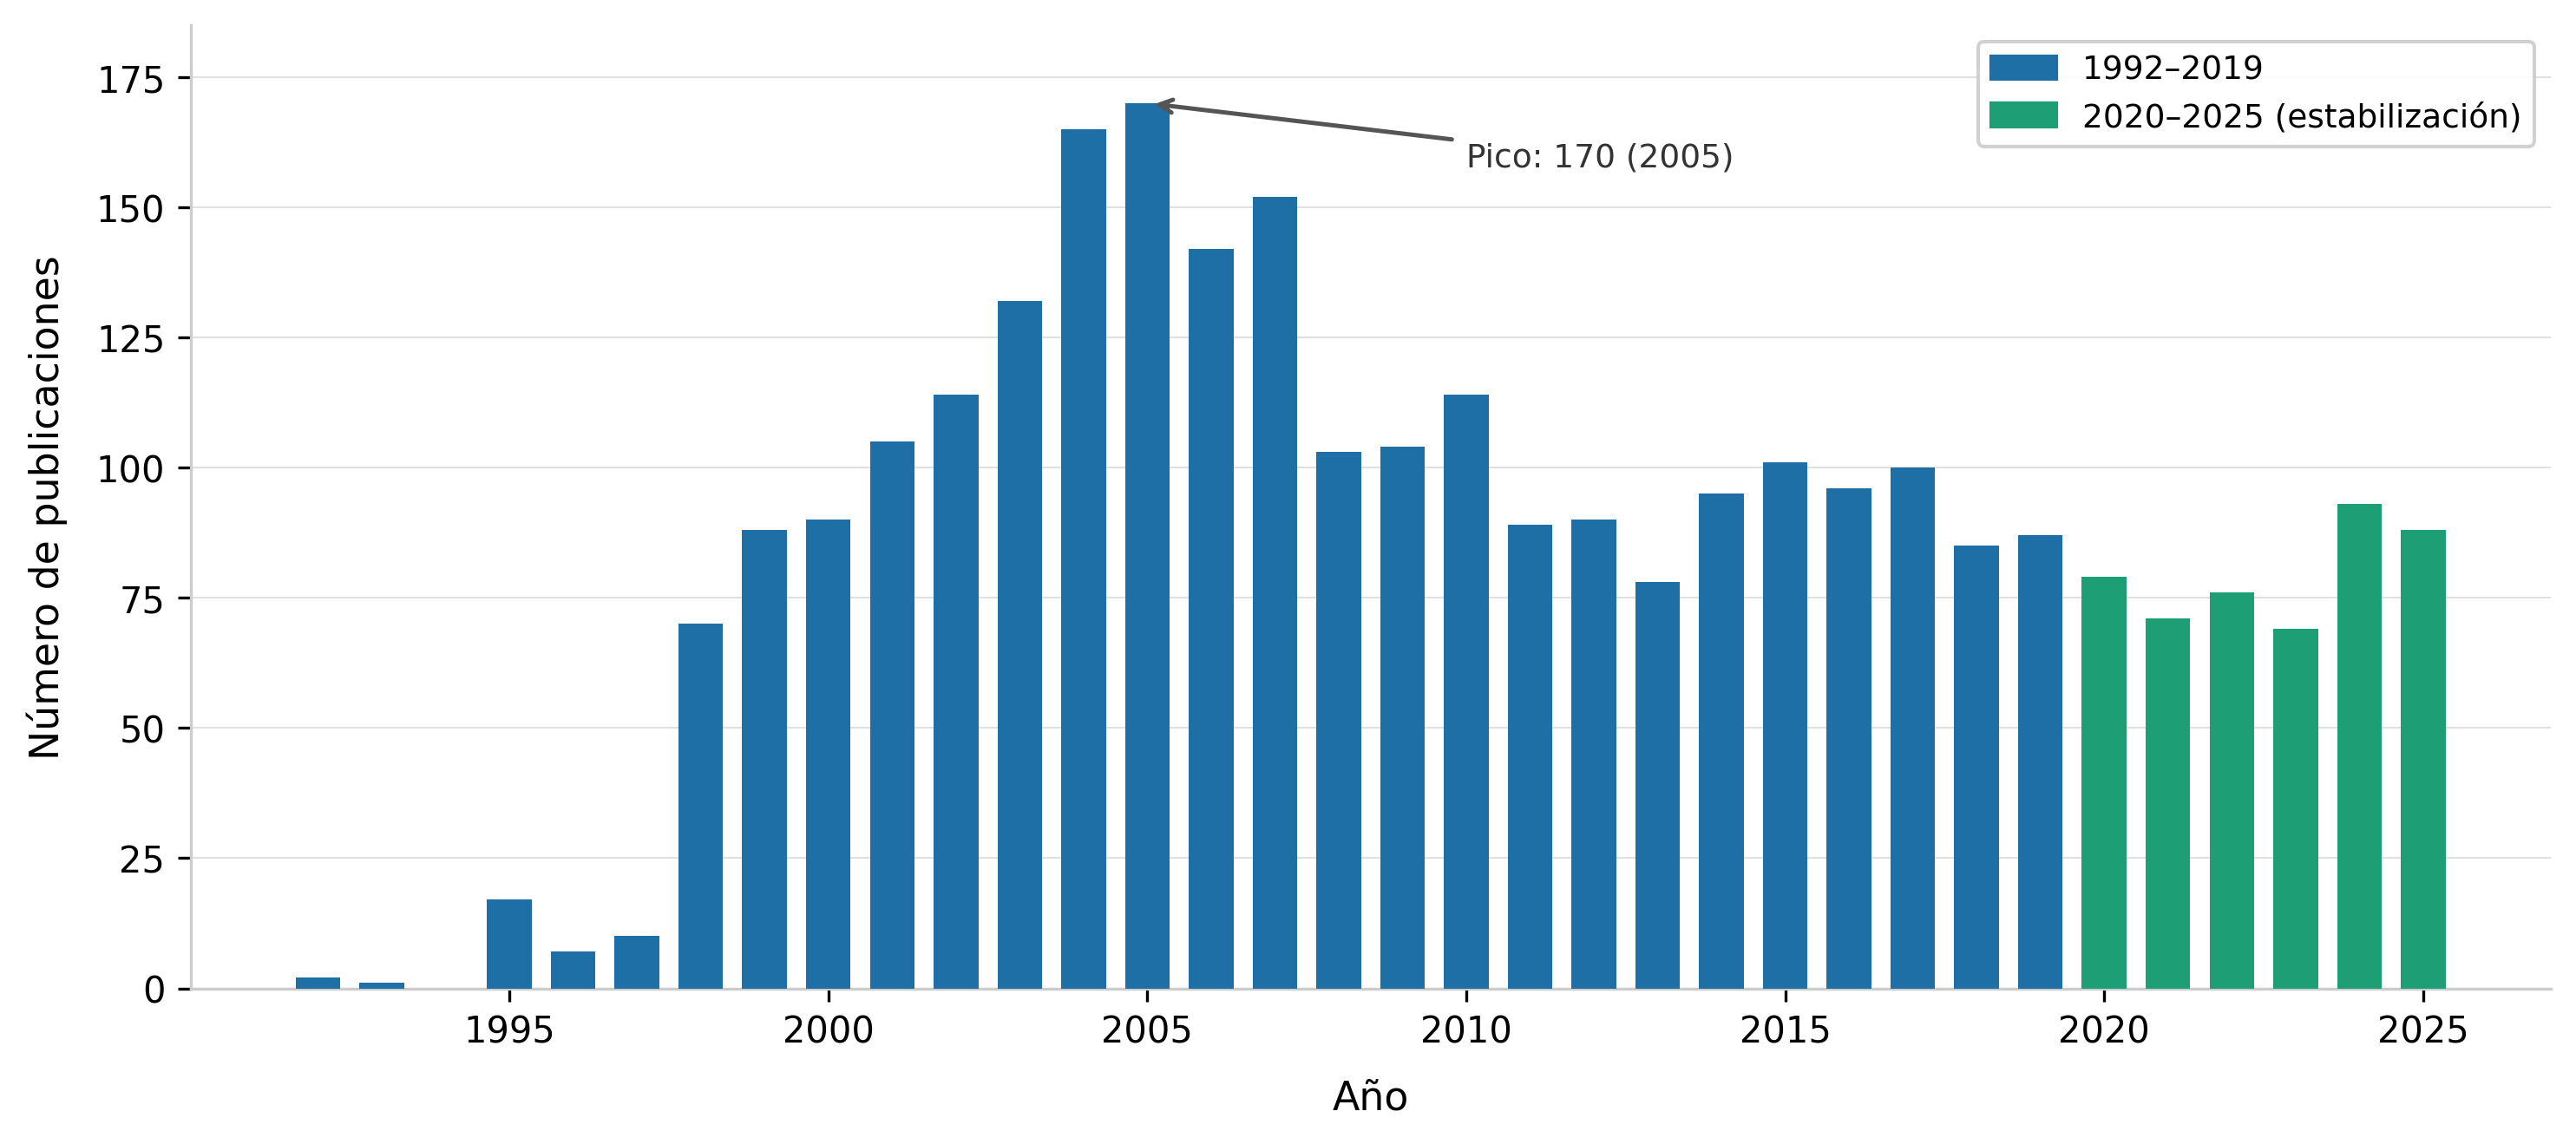
\includegraphics[width=0.92\textwidth]{figuras/tendencia_scopus.png}
  \caption{Tendencia de publicaciones sobre detección de \ac{MAP} en Scopus
           (palabras clave: \textit{landmine AND detection}). Se observa un
           pico máximo en 2004--2005 y una estabilización en torno a las
           80 publicaciones anuales en el período 2020--2025.}
  \label{fig:tendencia_scopus}

  {\footnotesize Fuente: elaboración propia con base en datos de Scopus.}
\end{figure}

Adicionalmente, de la revisión realizada por el grupo \ac{PSI}, un aspecto
diferenciador relevante es que ninguno de los trabajos con imágenes multiespectrales
o hiperespectrales identificados reporta experimentos con minas enterradas en
condiciones de siembra real prolongada ---es decir, con vegetación en crecimiento
libre durante semanas o meses sobre las zonas de mina---. El trabajo previo del
grupo \ac{PSI} con termografía infrarroja \cite{tenorio2024} sí opera en campo
real, pero explota la señal térmica aguda generada horas después del enterramiento,
no el estrés vegetal crónico acumulado. Este trabajo incluye esa condición de siembra prolongada, más representativa
del desminado humanitario real, donde las minas permanecen enterradas
por años.

De la revisión bibliográfica realizada es posible identificar cuatro métodos
predominantes de localización de \ac{MAP}: el \ac{GPR}, los \ac{MD}, las
cámaras infrarrojas y las cámaras multiespectrales. El \ac{GPR} emite pulsos
electromagnéticos que detectan cambios en las propiedades dieléctricas del
subsuelo, pero requiere operar muy cerca del terreno peligroso. Los \ac{MD}
son poco eficaces con minas de fabricación artesanal de contenido metálico
mínimo. Las cámaras infrarrojas y multiespectrales fundamentan su
funcionamiento en el procesamiento de imágenes capturadas en distintas
bandas del espectro, ofreciendo detección a distancia sin contacto con el
terreno \cite{barnawi2022}.

\subsection{Antecedentes internacionales}

A nivel internacional, el uso de imágenes multiespectrales e hiperespectrales
para la detección remota de \ac{MAP} ha ganado fuerza desde los años 90.

Un trabajo pionero es el de Clark \etal{} \cite{clark2000}, quienes
utilizaron una cámara Xybion de \textbf{seis bandas espectrales} (400--900~nm,
solo espectro visible) montada en un helicóptero para detectar minas
\textbf{metálicas, plásticas y sustitutos}, principalmente en superficie.
Su metodología extrae 54 características estadísticas (9 por banda) y selecciona
las más discriminativas mediante Sequential Forward Selection, utilizando una red
neuronal probabilística como clasificador. Con un conjunto de datos pequeño y en
condiciones de laboratorio, logró una Probabilidad de Detección (PD~=~1.0) ---
equivalente a una sensibilidad del 100\,\%--- y una Probabilidad de Falsa Alarma
(PFA~=~0.036) entrenando con minas metálicas y plásticas combinadas. Estos
resultados, aunque prometedores, fueron obtenidos en condiciones controladas sin
vegetación real, lo que limita su comparación directa con el presente trabajo.
Esta metodología de extracción de características estadísticas por banda es el
antecedente metodológico más directo del presente trabajo.

Makki \etal{} \cite{makki2017} presentaron una revisión sistemática de los
métodos de detección mediante imágenes hiperespectrales, demostrando que
la respuesta espectral de las minas con carcasa de plástico difiere de la
reflectancia del material de fondo, con tasas de detección reportadas en la
literatura superiores al 90\,\% en condiciones controladas. En su tesis doctoral
\cite{makki2017thesis}, el mismo autor desarrolló métodos de procesamiento
hiperespectral y reducción de dimensionalidad, señalando que la alta cantidad
de bandas de los sensores hiperespectrales requiere estrategias de selección
de características para ser operativos en campo --- motivación directa para el
uso de cámaras multiespectrales de pocas bandas seleccionadas.

Silva \etal{} \cite{silva2019} compararon clasificadores convencionales
contra una \ac{CNN} utilizando una cámara multiespectral Quest Condor3 de
\textbf{tres canales} (400--1000~nm) más una cámara térmica FLIR, en estructura
fija de laboratorio y campo exterior. Trabajaron con minas \textbf{antipersona
y antitanque plásticas} en suelo de arena (0--50~mm de profundidad), logrando
exactitud del 97\,\% en ambientes controlados. Evidenciaron que la profundidad
de enterramiento y las condiciones del entorno influyen significativamente en la
eficacia.
A diferencia de Silva \etal{}, aquí se trabaja con vegetación en crecimiento libre
y profundidades de hasta 70~mm en terreno de campo real.

Qiu \etal{} \cite{qiu2023} propusieron un sistema en \ac{UAV} con cámara
Sequoia de \textbf{cuatro bandas} (Verde, Rojo, Red Edge, NIR) y fusión YOLOv5,
logrando recall de 0.906 con RGB+NIR frente a 0.848 con RGB solo, demostrando la
ventaja de incorporar NIR. Vivoli \etal{} \cite{vivoli2024} implementaron detección
en tiempo real de minas superficiales con imágenes RGB y YOLO, superando el
90\,\% en campo real.

\subsection{Antecedentes nacionales}

En Colombia, la lucha contra las \ac{MAP} ha impulsado diversas
iniciativas de investigación centradas en técnicas de detección adaptadas
a las particularidades del conflicto y el terreno nacional.

Los trabajos más relevantes son los del grupo \ac{PSI}, que comparten el
mismo tipo de mina, terreno y condiciones de campo. Forero \etal{}
\cite{forero2022} lograron detectar \ac{MAP} tipo quiebrapatas con sensibilidad
del 97.1\,\% usando una cámara termográfica en \ac{UAV} a \SI{1}{m} y un
clasificador \ac{MLP}. Tenorio \etal{} \cite{tenorio2024} ampliaron el estudio
a alturas de 1--5~m, logrando exactitud del 92.13\,\% y sensibilidad del
82.4\,\% sobre 260 imágenes de prueba. A diferencia del enfoque térmico ---que
detecta contraste de temperatura agudo y depende del horario de captura---,
el enfoque multiespectral propuesto detecta perturbaciones crónicas del suelo y
la vegetación, con señal más estable temporalmente.

Cardona \etal{} \cite{cardona2014} revisaron tecnologías de detección en
Antioquia, identificando los \ac{MD}, el \ac{GPR} y las cámaras infrarrojas
y multiespectrales como las más viables para el contexto colombiano. Tovar
\cite{tovar2017} exploró la fusión de datos de múltiples sensores para
determinar la presencia de \ac{MAP} en una tesis de maestría de 2017;
aunque concluye que la combinación de sensores mejora la tasa de detección,
no reporta métricas numéricas comparables con los demás trabajos revisados,
no trabaja específicamente con imágenes multiespectrales, y sus condiciones
de experimentación no son equiparables a las del presente trabajo.

\subsection{Discusión de antecedentes}

La Tabla~\ref{tab:antecedentes} sintetiza los trabajos más relevantes,
cubriendo los aspectos metodológicos clave que permiten compararlos con el
presente trabajo.

\begin{table}[H]
\centering
\caption{Comparación de trabajos de referencia en detección de \ac{MAP}}
\label{tab:antecedentes}
\footnotesize
\begin{adjustbox}{width=1.15\textwidth,center}
\begin{tabular}{p{2.0cm}p{2.2cm}p{2.4cm}p{2.0cm}p{1.4cm}p{2.2cm}}
\toprule
\textbf{Trabajo} & \textbf{Sensor} & \textbf{Clasif.} &
\textbf{Métrica} & \textbf{Altura} & \textbf{Plataforma / entorno} \\
\midrule
Clark \etal{} \cite{clark2000}
  & MS 6 bandas & PNN & PD=1.0, PFA=0.036 & 76--137 m & Avión, exterior \\
Silva \etal{} \cite{silva2019}
  & MS 3 canales & SVM / CNN & OA 97\,\% & N/E & Estructura fija, lab./campo \\
Forero \etal{} \cite{forero2022}
  & Térmica IR & MLP & Sens. 97.1\,\% & 1 m & UAV, campo real \\
Tenorio \etal{} \cite{tenorio2024}
  & Térmica IR & MLP & Sens. 82.4\,\% & 1--5 m & UAV, campo real \\
Qiu \etal{} \cite{qiu2023}
  & MS 4 bandas & YOLOv5 & Recall 0.906 & N/E & UAV, campo real \\
Vivoli \etal{} \cite{vivoli2024}
  & Espectro visible & YOLO & Prec./Recall $>$90\,\% & N/E & UAV, tiempo real \\
\midrule
\textbf{Este trabajo}
  & \textbf{MS 5 bandas} & \textbf{EasyEns.~x10 XGBoost} & \textbf{AUC 0.947 / Sens. 82.3\,\%} & \textbf{1 m} & \textbf{Soporte estac., campo real} \\
\bottomrule
\multicolumn{6}{l}{\small MS: Multiespectral; estac.: sistema estacionario; N/E: no especificada.} \\
\multicolumn{6}{l}{\small OA: Overall Accuracy; Sens.: Sensibilidad; PD: Prob. Detección; PFA: Prob. Falsa Alarma.} \\
\multicolumn{6}{l}{\small AUC calculado con validación LOSO; Sens. con umbral fijo~=~0.5 (EasyEnsemble).} \\
\multicolumn{6}{l}{\small Los demás trabajos reportan métricas con partición aleatoria o conjunto de prueba fijo.}
\end{tabular}
\end{adjustbox}

  {\footnotesize Fuente: elaboración propia.}
\end{table}

Las Tablas~\ref{tab:comparacion_ms_features} y~\ref{tab:comparacion_ms_dataset}
profundizan la comparación exclusivamente entre los trabajos que emplean imágenes
multiespectrales, analizando aspectos técnicos directamente comparables con el
presente trabajo: el tipo y cantidad de características extraídas, el método de
selección y los parámetros del clasificador (Tabla~\ref{tab:comparacion_ms_features}),
así como el tamaño y balance del dataset, la estrategia de validación y las
condiciones de terreno y enterramiento (Tabla~\ref{tab:comparacion_ms_dataset}).
Esta comparación ubica los aportes metodológicos del presente trabajo
respecto al estado del arte multiespectral.

\clearpage
\begin{landscape}
\begin{table}
\centering
\caption{Comparación técnica (parte 1): características y clasificadores ---
         trabajos con imágenes multiespectrales para detección de \ac{MAP}}
\label{tab:comparacion_ms_features}
\footnotesize
\begin{tabularx}{\linewidth}{p{1.8cm} X X X p{2.5cm}}
\toprule
\textbf{Trabajo} & \textbf{Características extraídas} &
\textbf{Método de selección} & \textbf{Clasificador y parámetros clave} &
\textbf{Tamaño de ventana/ROI} \\
\midrule
Clark \etal{} \cite{clark2000}
  & 54 features: 9 estadísticas por banda (máx., mín., rango, media, std,
    asimetría, curtosis, energía, entropía) × 6 bandas
  & Sequential Forward Selection (SFS) con distancia de Bhattacharyya;
    se seleccionan 3 features finales
  & Red Neuronal Probabilística (PNN); parámetro $\sigma$ optimizado por
    tipo de mina; postprocesamiento por tamaño y forma
  & Tile 5×5 px por banda \\
\addlinespace
Silva \etal{} \cite{silva2019}
  & 264 features: estadísticas de orden superior + GLCM (textura:
    contraste, energía, correlación, homogeneidad a 0°, 45°, 90°, 135°)
    + índices espectrales
  & Algoritmo Relief (\textit{método de filtro}); features normalizadas
    al rango [0,\,1]
  & SVM kernel polinomial grado 8, algoritmo ISDA (\textit{Iterative Single Data Algorithm}, mejor exactitud);
    CNN con 3 capas conv. (filtros 64/128/256), batch norm., ReLU,
    pooling; hasta 200 épocas
  & ROI 10×10 px (AP); 80×80 px (AT) \\
\addlinespace
Qiu \etal{} \cite{qiu2023}
  & Mapas de características generados automáticamente por la CNN
    (no hay extracción manual de features)
  & Implícita en la arquitectura CNN (YOLOv5)
  & YOLOv5 \textit{end-to-end}; alturas de vuelo 3 y 8~m;
    solapamiento de imágenes 80\,\%
  & N/E (detección directa sobre imagen completa) \\
\addlinespace
\textbf{Este trabajo}
  & \textbf{378 features: 9 estadísticas (media, std, p25, p50, p75,
    mín., máx., mediana, rango) × 42 índices espectrales de
    vegetación, suelo y humedad (NDVI, NDRE, EVI, NDWI, BSI, SAVI\ldots)}
  & \textbf{Importancia de ganancia XGBoost (\textit{embedded}, undersampling 1:1 por fold);
    top-70 de 378; óptimo determinado por curva AUC/Sens vs.\ $k$}
  & \textbf{EasyEnsemble~x10 XGBoost (10 sub-clasificadores, ratio~1:1);
    RF y SVM~RBF evaluados como comparación base}
  & \textbf{Ventana 128×128 px; solapamiento 50\,\%} \\
\bottomrule
\multicolumn{5}{l}{\small SFS: Sequential Forward Selection; GLCM: Gray Level Co-occurrence Matrix;
Relief: filtro basado en distancias entre instancias.} \\
\multicolumn{5}{l}{\small PNN: red neuronal probabilística; CNN: red neuronal convolucional;
AP: antipersona; AT: antitanque; N/E: no especificado.}
\end{tabularx}

  {\footnotesize Fuente: elaboración propia.}
\end{table}
\end{landscape}
\clearpage


\clearpage
\begin{landscape}
\begin{table}
\centering
\caption{Comparación técnica (parte 2): dataset, validación y condiciones experimentales ---
         trabajos con imágenes multiespectrales para detección de \ac{MAP}}
\label{tab:comparacion_ms_dataset}
\footnotesize
\begin{tabularx}{\linewidth}{p{1.8cm}X X p{2.0cm} X}
\toprule
\textbf{Trabajo} & \textbf{Tamaño y balance del dataset} &
\textbf{Estrategia de validación} & \textbf{Métrica} &
\textbf{Condiciones de terreno y minas} \\
\midrule
Clark \etal{} \cite{clark2000}
  & $\sim$100 muestras mina, $\sim$200 fondo (balance 1:2);
    reconocido por los autores como dataset pequeño
  & Hold-one-out durante entrenamiento; conjunto de prueba
    fijo separado
  & PD=1.0 PFA=0.036
  & Campo militar real con pasto, arena y zonas despejadas;
    minas principalmente en superficie (pocas enterradas);
    mezcla de minas metálicas, plásticas y sustitutos;
    sin control de vegetación ni tiempo de enterramiento \\
\addlinespace
Silva \etal{} \cite{silva2019}
  & AP indoor: 10,262 ROIs; AP outdoor: 7,056 ROIs;
    \textbf{balanceado artificialmente}
  & Holdout 85\,\% entreno / 15\,\% prueba (partición aleatoria)
  & OA 97\,\% Sens. 98.5\,\%
  & Arena de laboratorio (cajones indoor) y academia militar
    (outdoor); profundidades AP $\leq$5~mm, AT $\leq$10~mm;
    objetos enterrados $<$30~min \textbf{(sin señal crónica
    acumulada)}; suelo perturbado no detectado por el sistema \\
\addlinespace
Qiu \etal{} \cite{qiu2023}
  & 789 pares de imágenes;
    minas en superficie o semisuperficiales
  & N/E
  & Recall 0.906
  & Pasto natural con vegetación variable; $\sim$60\,\% de las
    minas cubiertas por vegetación; minas en superficie
    (no enterradas); alturas de vuelo 3 y 8~m \\
\addlinespace
\textbf{Este trabajo}
  & \textbf{14,901 ventanas; 487 positivos / 14,414 negativos;
    desbalance real 30:1 (no balanceado artificialmente)}
  & \textbf{LOSO con 6 sesiones de campo --- sin fuga de datos
    entre sesiones; validación cruzada aleatoria descartada
    (AUC=0.999 inflado; véase Sección~\ref{sec:loso})}
  & \textbf{AUC 0.947 Sens. 82.3\,\% (umbral~=~0.5)}
  & \textbf{Campo real con vegetación limitada en crecimiento
    libre $\sim$6~meses; minas enterradas 1--7~cm;
    objetos de interferencia enterrados a la misma profundidad;
    señal crónica confirmada en bandas NIR} \\
\bottomrule
\multicolumn{5}{l}{\small OA: Overall Accuracy; Sens.: Sensibilidad con umbral fijo~=~0.5 (EasyEnsemble);
N/E: no especificado; AP: antipersona; AT: antitanque.} \\
\multicolumn{5}{l}{\small Las métricas de Silva et al. se obtuvieron con dataset balanceado artificialmente;
las de este trabajo con desbalance real y validación LOSO.}
\end{tabularx}

  {\footnotesize Fuente: elaboración propia.}
\end{table}
\end{landscape}
\clearpage
Los trabajos del grupo \ac{PSI} \cite{forero2022,tenorio2024} son el
referente más directo: mismo tipo de mina, mismo terreno experimental y
vegetación real. Este trabajo añade el análisis multiespectral a esa línea,
con una señal distinta
a la térmica.

Un aspecto diferenciador frente a los antecedentes revisados es la contribución
discriminativa de las bandas Red Edge y \ac{NIR}, observada con el etiquetado
preciso por bounding box ---aspecto poco explorado en los trabajos previos. Además, Clark~\etal{} y Silva~\etal{} operaron sin vegetación
real; este trabajo se realizó en campo con vegetación en crecimiento libre.

% -------------------------------------------------------------
\section{Mina Antipersona}

Las \ac{MAP} son artefactos explosivos diseñados para detonarse por la
presencia o proximidad de una persona, con el fin de incapacitarla,
herirla o matarla. Se activan típicamente al ser pisadas o al tensar un
cable trampa que libera una carga explosiva. En Colombia se ha identificado
gran variedad de minas, de las cuales más del 90\,\% son de fabricación
artesanal \cite{ocha2015,unicef2021}.

\subsection{Tipos de minas antipersona más comunes en Colombia}

La mayoría de \ac{MAP} colombianas son de fabricación artesanal e
improvisada, con mínimos componentes metálicos, fabricadas con materiales
de fácil acceso como madera, tubos de \ac{PVC}, plásticos, fragmentos de
metal, vidrios y explosivos caseros \cite{mineban2010,gutierrez2014}:

\textbf{Mina quiebrapatas.} La más común y la que más víctimas cobra \cite{hernandez2023}.
Diseñada para explotar cuando es pisada, fabricada con tubo de \ac{PVC},
alambre, batería de 1.5~V, explosivo (dinamita o nitrato de amonio) y
fragmentos de metal. Es el tipo de mina emulada en el presente trabajo.

\textbf{Mina tipo sombrero chino.} Rango efectivo de \SI{25}{m}.
Fabricada con explosivo casero R-1 y trozos de metal, con sistema de
activación eléctrico mediante cable conductor de 200 a 300~m.

\textbf{Mina tipo cajón.} Elaborada con caja de madera y dinamita o
explosivo casero R-1. Utilizada principalmente contra vehículos.

La predominancia de materiales no metálicos es la razón por la cual los
detectores de metales convencionales son ineficaces para la mayoría de las
\ac{MAP} colombianas, justificando la búsqueda de métodos de detección
alternativos basados en propiedades ópticas y espectrales.

% -------------------------------------------------------------
\section{Tipos de suelos}

El territorio colombiano comprende una amplia variedad de suelos determinados
por su diversidad geográfica y climática. En las zonas de alta presencia de
\ac{MAP} predominan suelos arcillosos y franco-arcillosos, suelos con alto
contenido orgánico en áreas selváticas tropicales y suelos arenosos
\cite{IsaacAnteproyecto}.

Este trabajo se enfoca en suelos con textura arenosa y vegetación limitada,
condición del terreno experimental utilizado en el campus de la Universidad
del Valle, sede Meléndez --- el mismo terreno empleado en los trabajos previos
del grupo \ac{PSI} \cite{forero2022,tenorio2024}. El contraste espectral
entre el suelo perturbado (sobre la mina) y el suelo sin alteración es más
pronunciado en suelos de textura gruesa, donde la remoción del material
durante el enterramiento genera cambios de color y textura superficial más
evidentes que en suelos arcillosos compactos \cite{nanni2006}.

% -------------------------------------------------------------
\section{Imágenes multiespectrales}

A diferencia de una cámara convencional RGB, un sensor multiespectral
captura información en múltiples bandas del espectro electromagnético.
La cámara produce varias imágenes de la misma escena, cada una
correspondiente a una banda específica de longitudes de onda; al
superponer o analizar conjuntamente las bandas, es posible distinguir
objetos o características que pasan desapercibidas al analizar únicamente el espectro visible
\cite{navarro2024}.

\subsection{La cámara MicaSense RedEdge-MX}

Para este trabajo se empleó la cámara MicaSense RedEdge-MX, que captura
imágenes en cinco bandas espectrales con resolución de 1.2~Mpx por banda.
Las características de cada banda se resumen en la
Tabla~\ref{tab:bandas_micasense}.

\begin{table}[H]
\centering
\caption{Especificaciones de las bandas de la cámara MicaSense RedEdge-MX}
\label{tab:bandas_micasense}
\begin{tabular}{clcc}
\toprule
\textbf{Banda} & \textbf{Nombre} & \textbf{Centro (\si{nm})} &
\textbf{Ancho FWHM (\si{nm})} \\
\midrule
1 & Azul (Blue)              & 475 & 32 \\
2 & Verde (Green)            & 560 & 27 \\
3 & Rojo (Red)               & 668 & 16 \\
4 & Red Edge                 & 717 & 12 \\
5 & Infrarrojo Cercano (NIR) & 842 & 57 \\
\bottomrule
\end{tabular}

  {\footnotesize Fuente: elaboración propia.}
\end{table}

La cámara dispone de cinco objetivos físicamente separados, uno por banda,
lo que implica que las imágenes de cada banda requieren un proceso de
corrección geométrica (Sección~\ref{sec:alineacion}).

\subsection{Firma espectral y mecanismos de detección de MAP}

Los distintos materiales reflejan o emiten radiación de manera diferente
en cada banda espectral; a esto se denomina \textit{firma espectral}.
En el caso de una \ac{MAP} enterrada, la anomalía espectral puede
manifestarse de tres formas principales \cite{qiu2023,barnawi2022}:

\textbf{Perturbación del color superficial del suelo.} El proceso de
enterramiento remueve y redeposita el material del suelo, alterando su
composición superficial. El suelo subsuperficial expuesto tiene una
composición mineralógica y un contenido de materia orgánica diferente al
suelo superficial original, generando diferencias de color detectables en
las bandas del espectro visible (Azul, Verde, Rojo). Este mecanismo opera
desde el momento del enterramiento y produce señales espectrales en índices
como \ac{VARI}, \ac{NDRB} y el ratio Rojo/Azul.

\textbf{Estrés vegetal diferencial — señal en Red Edge y NIR.}
Las plantas sobre una \ac{MAP} enterrada pueden responder al estrés mecánico
(compactación del suelo) y químico del material explosivo, generando cambios
en su contenido de clorofila y en la estructura del mesófilo foliar. La
clorofila absorbe fuertemente en las bandas roja y azul, y refleja en la
banda verde; cuando el contenido de clorofila disminuye por estrés, la
reflectancia en la banda \textbf{Red Edge} (\SI{717}{nm}) aumenta de forma
característica antes de que el estrés sea visible a simple vista
\cite{qiu2023}. La banda \textbf{\ac{NIR}} (\SI{842}{nm}) es sensible a la
estructura interna de la hoja (mesófilo): el estrés hídrico y mecánico
reduce la reflectancia \ac{NIR} al afectar los espacios de aire intercelulares
que generan la alta reflectancia infrarroja de la vegetación sana. Índices
que combinan estas bandas —\ac{NDRE}, \ac{NDVI}, y ratios NIR/Red— son
los más sensibles para detectar este tipo de estrés crónico. Este mecanismo
es de naturaleza acumulativa y se intensifica semanas o meses después del
enterramiento.

\textbf{Contraste térmico.} Las minas tienen propiedades térmicas distintas
al suelo, generando diferencias de temperatura detectables en imágenes
infrarrojas térmicas \cite{forero2022,tenorio2024}. Su señal es aguda y
transitoria, complementaria a los mecanismos espectrales.

\textbf{Implicación metodológica.} La precisión del etiquetado del
groundtruth determina cuál de estos mecanismos captura preferentemente el
clasificador. Un etiquetado grueso (toda la zona como positiva) tiende a privilegiar la
perturbación del color del suelo ---señal visible y distribuida en toda el área---,
mientras que un etiquetado ajustado por bounding box preserva mejor la señal
localizada de Red Edge y \ac{NIR}. El análisis de importancia del
Capítulo~\ref{cap:resultados} es \emph{consistente} con esta hipótesis: esas bandas
figuran entre las características relevantes del modelo.

% -------------------------------------------------------------
\section{Índices espectrales}
\label{sec:indices_espectrales}

Los índices espectrales son combinaciones matemáticas de dos o más bandas
diseñadas para resaltar características específicas de la superficie.
Los índices calculados en este trabajo se describen a continuación.

\subsection{Índices de vegetación}

El \ac{NDVI} es el índice de vegetación más ampliamente utilizado en
teledetección \cite{makki2017}:
\begin{equation}
  \text{NDVI} = \frac{\rho_{\text{NIR}} - \rho_{\text{Red}}}
                     {\rho_{\text{NIR}} + \rho_{\text{Red}}}
  \label{eq:ndvi}
\end{equation}
Sus valores van de $-1$ a $+1$; por encima de 0.5 se asocia a vegetación
densa y sana, por debajo de 0.2 a suelo desnudo o agua.

El \ac{NDRE} es análogo al \ac{NDVI} pero utiliza la banda Red Edge
(\SI{717}{nm}) en lugar de la banda Roja. La región Red Edge corresponde
al borde de absorción de la clorofila, donde la reflectancia transiciona
abruptamente de baja (rojo, absorbido por clorofila) a alta (NIR, reflejado
por estructura celular). Cambios en el contenido de clorofila desplazan
este borde, haciendo al \ac{NDRE} más sensible que el \ac{NDVI} a estrés
vegetal temprano — cuando el estrés aún no es visible a simple vista
\cite{makki2017}:
\begin{equation}
  \text{NDRE} = \frac{\rho_{\text{NIR}} - \rho_{\text{RedEdge}}}
                     {\rho_{\text{NIR}} + \rho_{\text{RedEdge}}}
  \label{eq:ndre}
\end{equation}

La banda \ac{NIR} (\SI{842}{nm}) es particularmente sensible a la estructura
interna de la hoja: la alta reflectancia infrarroja de la vegetación sana
proviene de los espacios de aire entre células del mesófilo, que actúan como
dispersores de radiación. El estrés hídrico y mecánico colapsa estos espacios,
reduciendo la reflectancia \ac{NIR}. Por esta razón, índices que involucran
\ac{NIR} —como \ac{NDVI}, \ac{NDRE} y el ratio NIR/Red— son los más
discriminativos para detectar estrés vegetal crónico inducido por el
enterramiento de \ac{MAP}.

El \ac{EVI} reduce el efecto del suelo de fondo y la saturación
atmosférica en zonas de alta densidad vegetal:
\begin{equation}
  \text{EVI} = 2.5 \cdot
  \frac{\rho_{\text{NIR}} - \rho_{\text{Red}}}
       {\rho_{\text{NIR}} + 6\,\rho_{\text{Red}} - 7.5\,\rho_{\text{Blue}} + 1}
  \label{eq:evi}
\end{equation}

El \ac{VARI} estima la fracción de cobertura vegetal usando exclusivamente
bandas visibles, siendo robusto ante variaciones de irradiancia. Es el
índice más discriminativo identificado en este trabajo:
\begin{equation}
  \text{VARI} = \frac{\rho_{\text{Green}} - \rho_{\text{Red}}}
                     {\rho_{\text{Green}} + \rho_{\text{Red}} - \rho_{\text{Blue}}}
  \label{eq:vari}
\end{equation}

\subsection{Índices de ratio entre bandas visibles}

El \ac{NDRB} cuantifica la diferencia normalizada entre las bandas roja
y azul, sensible a cambios en el color superficial del suelo:
\begin{equation}
  \text{NDRB} = \frac{\rho_{\text{Red}} - \rho_{\text{Blue}}}
                     {\rho_{\text{Red}} + \rho_{\text{Blue}}}
  \label{eq:ndrb}
\end{equation}

El \ac{NDGB} compara las bandas verde y azul, sensible a cambios en la
composición superficial del suelo:
\begin{equation}
  \text{NDGB} = \frac{\rho_{\text{Green}} - \rho_{\text{Blue}}}
                     {\rho_{\text{Green}} + \rho_{\text{Blue}}}
  \label{eq:ndgb}
\end{equation}

El ratio Rojo/Azul es un indicador directo del color del suelo; suelos con
mayor contenido de óxidos de hierro o materia orgánica alterada presentan
valores más altos:
\begin{equation}
  \text{Red/Blue} = \frac{\rho_{\text{Red}}}{\rho_{\text{Blue}}}
  \label{eq:redblue}
\end{equation}

\subsection{Índices de suelo y textura}

El \ac{BSI} resalta áreas de suelo desnudo combinando múltiples bandas:
\begin{equation}
  \text{BSI} = \frac{(\rho_{\text{Red}} + \rho_{\text{Blue}}) -
                     (\rho_{\text{NIR}} + \rho_{\text{Green}})}
                    {(\rho_{\text{Red}} + \rho_{\text{Blue}}) +
                     (\rho_{\text{NIR}} + \rho_{\text{Green}})}
  \label{eq:bsi}
\end{equation}

El \ac{HI} cuantifica el tono de color del suelo en el espacio visible,
siendo sensible a cambios en la mineralogía superficial y el contenido de
materia orgánica:
\begin{equation}
  \text{HI} = \frac{2\,\rho_{\text{Red}} - \rho_{\text{Green}} - \rho_{\text{Blue}}}
                   {2(\rho_{\text{Red}} - \rho_{\text{Blue}})}
  \label{eq:hi}
\end{equation}

El \textbf{NDSI} (\textit{Normalized Difference Soil Index}) cuantifica la
proporción entre la reflectancia roja y el infrarrojo cercano, siendo
sensible a la exposición de suelo desnudo y a perturbaciones superficiales:
\begin{equation}
  \text{NDSI} = \frac{\rho_{\text{Red}} - \rho_{\text{NIR}}}
                     {\rho_{\text{Red}} + \rho_{\text{NIR}}}
  \label{eq:ndsi}
\end{equation}

% -------------------------------------------------------------
\section{Calibración radiométrica}
\label{sec:calibracion_teorica}

La calibración radiométrica transforma los valores de nivel digital~(DN)
capturados por el sensor en valores de reflectancia de superficie,
independientes de las condiciones de iluminación. Sin calibración, los
valores de DN varían entre sesiones según la hora del día, la nubosidad
y el ángulo solar, impidiendo comparar imágenes de distintos momentos.

El método empleado utiliza un \ac{CRP}, que es un panel de material
difusamente reflectante con valores de reflectancia nominal conocidos y
certificados para cada banda espectral: Blue~=~0.490, Green~=~0.491,
Red~=~0.491, Red Edge~=~0.488 y NIR~=~0.490. Estos valores, proporcionados
por el fabricante, establecen la relación lineal entre el nivel digital
(DN) capturado por el sensor y la reflectancia de superficie real:
\begin{equation}
  \rho_{\text{sup}}(\lambda) =
  \frac{\text{DN}_{\text{zona}}(\lambda)}{\text{DN}_{\text{panel}}(\lambda)}
  \cdot \rho_{\text{panel}}(\lambda)
  \label{eq:calibracion}
\end{equation}
\noindent donde $\rho_{\text{panel}}(\lambda)$ es la reflectancia nominal
del panel para la banda $\lambda$.

% -------------------------------------------------------------
\section{Alineación de bandas}
\label{sec:alineacion}

Dado que la MicaSense RedEdge-MX contiene cinco objetivos físicamente
separados, las bandas no están perfectamente alineadas entre sí. A
\SI{1}{m} de altura, el paralaje entre lentes genera un desalineamiento
residual que debe corregirse para que los índices espectrales calculados
a nivel de píxel sean representativos.

La corrección geométrica entre bandas se realiza mediante \ac{SIFT}
\cite{sift_lowe2004}, algoritmo seleccionado por tres razones frente a
otras alternativas como ORB, SURF o correlación cruzada:
(1)~es invariante a cambios de escala,
rotación e iluminación entre bandas, condición importante dado que los
cinco lentes de la MicaSense capturan con ligeras diferencias de perspectiva
y exposición; (2)~produce descriptores robustos que funcionan bien en
texturas naturales como suelo y vegetación, a diferencia de métodos basados
en bordes (Harris, FAST) que requieren contornos bien definidos; y
(3)~permite estimar una homografía global mediante RANSAC, que corrige el
desplazamiento promedio entre bandas de forma eficiente con el conjunto de
datos disponible. Como alternativa cuando \ac{SIFT} no converge se utiliza
el algoritmo ECC (\textit{Enhanced Correlation Coefficient}), que opera por
optimización iterativa y es más robusto en imágenes con poco contraste.

A \SI{1}{m} de captura el paralaje entre los cinco lentes es
significativamente mayor que a distancias típicas de vuelo. La homografía
global corrige el desplazamiento promedio pero no puede compensar el
paralaje local generado por objetos tridimensionales como la vegetación.
Este efecto es inherente a la captura en campo cercano y es aceptable para
la extracción de características estadísticas por ventana.

% -------------------------------------------------------------
\section{Selección de características en teledetección}

En los trabajos de detección de \ac{MAP} con imágenes multiespectrales,
las características más empleadas son de naturaleza estadística y espectral.
Clark \etal{} \cite{clark2000} extrajeron estadísticas por banda (máximo,
media, curtosis, energía y desviación estándar) sobre regiones de interés,
seleccionando las más discriminativas mediante Sequential Forward Selection.
Silva \etal{} \cite{silva2019} utilizaron características de textura
derivadas de matrices de co-ocurrencia (GLCM) combinadas con índices
espectrales. Qiu \etal{} \cite{qiu2023} emplearon mapas de características
generados por redes convolucionales sobre composiciones multibanda. En el
presente trabajo se extraen estadísticas descriptivas (media,
desviación estándar, percentiles) sobre más de 40 índices espectrales de
vegetación, suelo y humedad calculados a partir de las cinco bandas de la
MicaSense RedEdge-MX, generando 378 características por ventana.

La selección de características es el proceso de identificar el subconjunto
mínimo de variables que preserva el poder predictivo del modelo completo.
En teledetección con datos de alta dimensionalidad cumple tres funciones:
reduce el sobreajuste al eliminar variables ruidosas o redundantes, mejora
la interpretabilidad del modelo identificando qué índices espectrales son
físicamente relevantes, y reduce el costo computacional de la clasificación.
Los métodos de selección de características se agrupan en tres familias
\cite{makki2017,silva2019}:

\begin{itemize}
  \item \textbf{Métodos de filtro:} evalúan cada característica de forma
    independiente mediante una métrica estadística (correlación, información
    mutua, Fisher Discriminant Ratio) y seleccionan las mejor puntuadas, sin
    intervención del clasificador. Son rápidos pero no capturan interacciones
    entre características.
  \item \textbf{Métodos envolventes (\textit{wrapper}):} utilizan el propio
    clasificador para evaluar subconjuntos de características por búsqueda
    exhaustiva o heurística (hacia adelante, hacia atrás). Son más precisos
    pero computacionalmente costosos.
  \item \textbf{Métodos embebidos:} la selección ocurre durante el
    entrenamiento del clasificador. El \ac{RF} pertenece a esta categoría:
    calcula la importancia de cada característica como la reducción media de
    impureza de Gini aportada a lo largo de todos los árboles del bosque
    \cite{breiman2001}.
\end{itemize}

En este trabajo se utiliza el método embebido de importancia por ganancia
de \ac{XGBoost} (reducción acumulada del error al dividir por cada
característica). La selección se realiza dentro del mismo clasificador final
(EasyEnsemble x10 XGBoost) y por cada fold de validación, con submuestreo
1:1, garantizando coherencia metodológica entre selección y clasificación.
Se seleccionan las 70 características de mayor importancia (\textit{top-70}).
A diferencia de Clark \etal{}, que aplicaron selección de características
sobre estadísticas de banda con un clasificador de red neuronal probabilística,
el presente trabajo combina el etiquetado preciso por bounding box con la
selección embebida de XGBoost; el análisis de importancia resultante es consistente
con una contribución discriminativa de las bandas Red Edge y \ac{NIR} ---aspecto
poco explorado en los trabajos revisados.

% -------------------------------------------------------------
\section{Algoritmos de clasificación}

La detección de \ac{MAP} se formula como un problema de clasificación
binaria supervisada: cada ventana se clasifica como \textit{con MAP} o
\textit{sin MAP}. A continuación se describen los algoritmos seleccionados
con base en su desempeño reportado en la literatura de teledetección y
detección de \ac{MAP} \cite{silva2019, barnawi2022, chen2016}.

\subsection{Bosque aleatorio (Random Forest)}

El \ac{RF} construye múltiples árboles de decisión durante el entrenamiento
y combina sus predicciones por votación mayoritaria \cite{breiman2001}.
Cada árbol se entrena sobre una muestra con reemplazo (\textit{bagging}),
y en cada nodo se selecciona aleatoriamente un subconjunto de
características, reduciendo la correlación entre árboles y mejorando la
generalización.

El \ac{RF} es el clasificador estándar en teledetección con bases de datos de
tamaño moderado \cite{silva2019} --- típicamente entre 1\,000 y 100\,000
muestras ---, rango que incluye la base de datos de este trabajo
(14\,901 ventanas). Sus propiedades son especialmente relevantes para este
problema: es invariante a la escala (no requiere normalización), robusto
con alta dimensionalidad (378 características), produce importancia de
características con valor interpretativo, y ofrece mecanismos para tratar
el desbalance de clases. A diferencia de
las redes neuronales profundas, generaliza bien con pocos miles de muestras
sin requerir grandes cantidades de datos de entrenamiento.

\subsection{Máquina de Vectores de Soporte (SVM)}

La \ac{SVM} busca el hiperplano de separación de máximo margen en el espacio
de características \cite{vapnik1995}. El núcleo RBF transforma implícitamente
el espacio a alta dimensión cuando los datos no son linealmente separables,
propiedad relevante para las 378 características espectrales del presente
trabajo. La \ac{SVM} requiere escalado previo; se aplica \texttt{StandardScaler}
ajustado dentro de cada pliegue \ac{LOSO} para evitar fuga de datos.

\subsection{XGBoost}

XGBoost (\textit{Extreme Gradient Boosting}) es un método de ensamble
basado en \textit{boosting}: construye árboles de decisión de forma
secuencial, donde cada árbol corrige los errores del anterior mediante
el gradiente de la función de pérdida \cite{chen2016}. A diferencia del \ac{RF} (árboles independientes por bagging), XGBoost
construye cada árbol corrigiendo los errores del anterior, lo que le
permite ajustarse a patrones más difíciles. En datos tabulares de alta
dimensionalidad, XGBoost supera al \ac{RF} cuando el volumen de datos es
suficiente \cite{qiu2023}. En este problema, las relaciones entre los índices
espectrales y la presencia de mina son altamente no lineales, lo que favorece a
XGBoost.

% -------------------------------------------------------------
\section{Estrategia de validación: Leave-One-Session-Out}
\label{sec:loso_teoria}

La estrategia de validación define cómo se reparten los datos entre
entrenamiento y prueba. Con partición aleatoria, ventanas de la misma imagen
pueden quedar en entrenamiento y prueba al mismo tiempo, inflando las
métricas ---en esta base de datos el AUC sube a 0.999 con partición
aleatoria frente a 0.947 con \ac{LOSO}---. En teledetección con sesiones
de campo, las condiciones ambientales de cada sesión correlacionan todas
las muestras de esa adquisición, haciendo el problema de fuga aún más
severo.

La estrategia \ac{LOSO} resuelve esto reservando en cada pliegue una sesión
de campo completa como conjunto de prueba y entrenando con las sesiones
restantes. Con $N$ sesiones se obtienen $N$ pliegues independientes, cada
uno evaluando la capacidad del modelo de generalizar a condiciones de
captura no vistas. Las métricas reportadas son el promedio de los $N$
pliegues. Esta estrategia es la recomendada en trabajos de detección
multiespectral donde la variabilidad entre sesiones de campo es la principal
fuente de incertidumbre \cite{silva2019}. Los detalles de implementación
para el presente trabajo se describen en la Sección~\ref{sec:loso}.
% ============================================================
%  CAPÍTULO 3 — DISEÑO METODOLÓGICO
% ============================================================
\chapter{Diseño Metodológico}

En este capítulo se describe la metodología utilizada para implementar el
sistema de detección de \ac{MAP} a partir del análisis de imágenes
multiespectrales aéreas del suelo. El diseño abarca cuatro etapas principales:
(1) construcción de la base de datos, (2) preprocesamiento radiométrico y
geométrico de las imágenes, (3) extracción de características espectrales, y
(4) clasificación y validación. La Figura~\ref{fig:pipeline_general} muestra
el diagrama general del \textit{pipeline} implementado.

\begin{figure}[H]
  \centering
  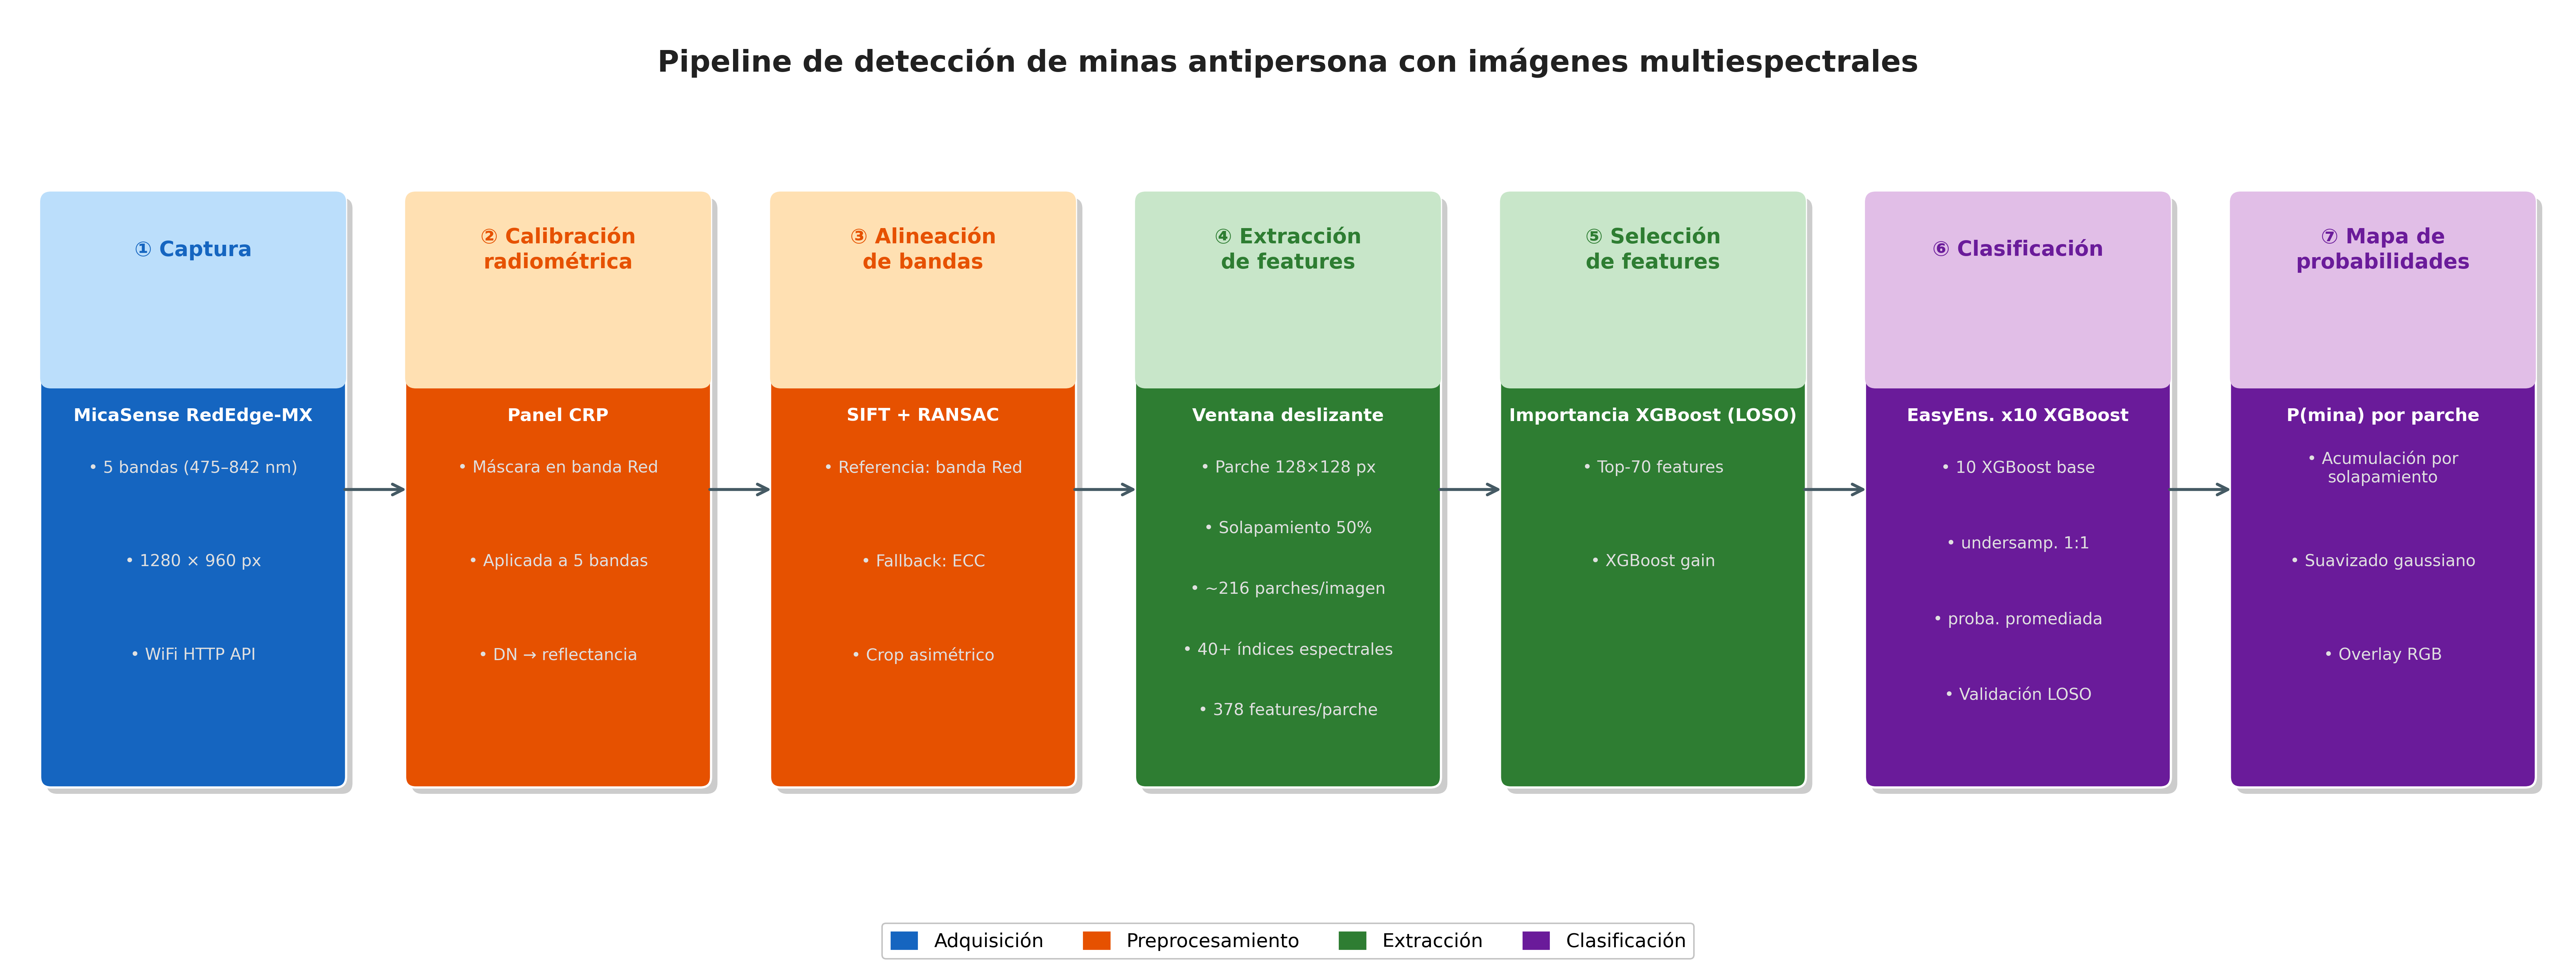
\includegraphics[width=\textwidth]{figuras/pipeline_general.png}
  \caption{Diagrama general del sistema de detección de \ac{MAP} propuesto.
           Las etapas se agrupan en cuatro categorías: adquisición (azul),
           preprocesamiento (naranja), extracción de características (verde)
           y clasificación (morado).}
  \label{fig:pipeline_general}

  {\footnotesize Fuente: elaboración propia.}
\end{figure}

% -------------------------------------------------------------
\section{Diseño del experimento}

\subsection{Construcción de las minas emuladas}

Para garantizar la seguridad durante la experimentación, se construyeron minas
emuladas que replican las características espectrales y morfológicas de las
\ac{MAP} tipo quiebrapatas, sin emplear material explosivo real. Siguiendo la
metodología establecida en \cite{forero2022}, cada mina se fabricó con los
siguientes componentes:

\begin{itemize}
  \item Cilindro externo de \ac{PVC} de \SI{10.2}{cm} de alto y
    \SI{7.62}{cm} de diámetro.
  \item \SI{400}{g} de carbón de antracita, como sustituto seguro del
    \ac{TNT}. La Tabla~\ref{tab:tnt_carbon} resume las propiedades térmicas
    de ambos materiales, evidenciando su similitud en calor específico y
    conductividad térmica \cite{forero2022}.
  \item \SI{20}{g} de clavos de acero, para simular los fragmentos metálicos
    presentes en las minas artesanales colombianas.
  \item Una pila de 9~V en el interior, para simular el sistema de activación
    eléctrico de la mina quiebrapatas real (que emplea una batería de 9~V
    como fuente de energía del detonador eléctrico). Este elemento diferencia
    las minas emuladas de este trabajo respecto al trabajo previo del grupo
    \ac{PSI} \cite{forero2022}, donde el detonador no incluía batería.
\end{itemize}

\begin{table}[H]
\centering
\caption{Propiedades térmicas del \ac{TNT} y del carbón de antracita \cite{forero2022}}
\label{tab:tnt_carbon}
\begin{tabular}{lcc}
\toprule
\textbf{Propiedad} & \textbf{TNT} & \textbf{Carbón de antracita} \\
\midrule
Densidad (\si{g/cm^3})             & 1.56 & 1.37 \\
Calor específico (\si{J/(g\cdot K)})   & 1.37 & 1.26 \\
Conductividad térmica (\si{W/(m\cdot K)}) & 0.26 & 0.23 \\
\bottomrule
\end{tabular}

  {\footnotesize Fuente: elaboración propia.}
\end{table}

El uso del carbón de antracita como sustituto del \ac{TNT} responde a dos
criterios. \textbf{Térmicamente}, sus propiedades similares de densidad, calor
específico y conductividad térmica lo hacen idóneo para replicar el contraste
infrarrojo de la mina real, siguiendo la metodología de los trabajos previos del
grupo \ac{PSI} \cite{forero2022,tenorio2024}. \textbf{Espectralmente}, el carbón
de antracita presenta baja reflectancia en el rango visible e infrarrojo cercano
sin características distintivas que puedan confundirse con la vegetación
\cite{barnawi2022}, lo que implica que el sistema no detecta el carbón directamente
sino las anomalías espectrales que su presencia induce en el suelo y la vegetación
circundantes --- el mecanismo en que se fundamenta la detección.

El mecanismo de activación se emula mediante una jeringa de \SI{5}{mL}
insertada en la tapa superior del cilindro. Al momento del enterramiento,
la cabeza del émbolo queda expuesta sobre la superficie del suelo ---
funcionalmente, es la parte que se pisa para activar la mina real ---,
por lo que en la base de datos definitiva se cubre con hojas u otro material
vegetal del entorno para evitar que sea visualmente distinguible desde la
cámara. Esta decisión de diseño fue determinante para la base de datos definitiva,
como se describe en la Sección~\ref{sec:iteracion_previa}.

La Figura~\ref{fig:minas_simuladas} muestra las minas emuladas construidas
para este experimento, con vista lateral y superior.

\begin{figure}[H]
  \centering
  \begin{subfigure}[b]{0.40\textwidth}
    \centering
    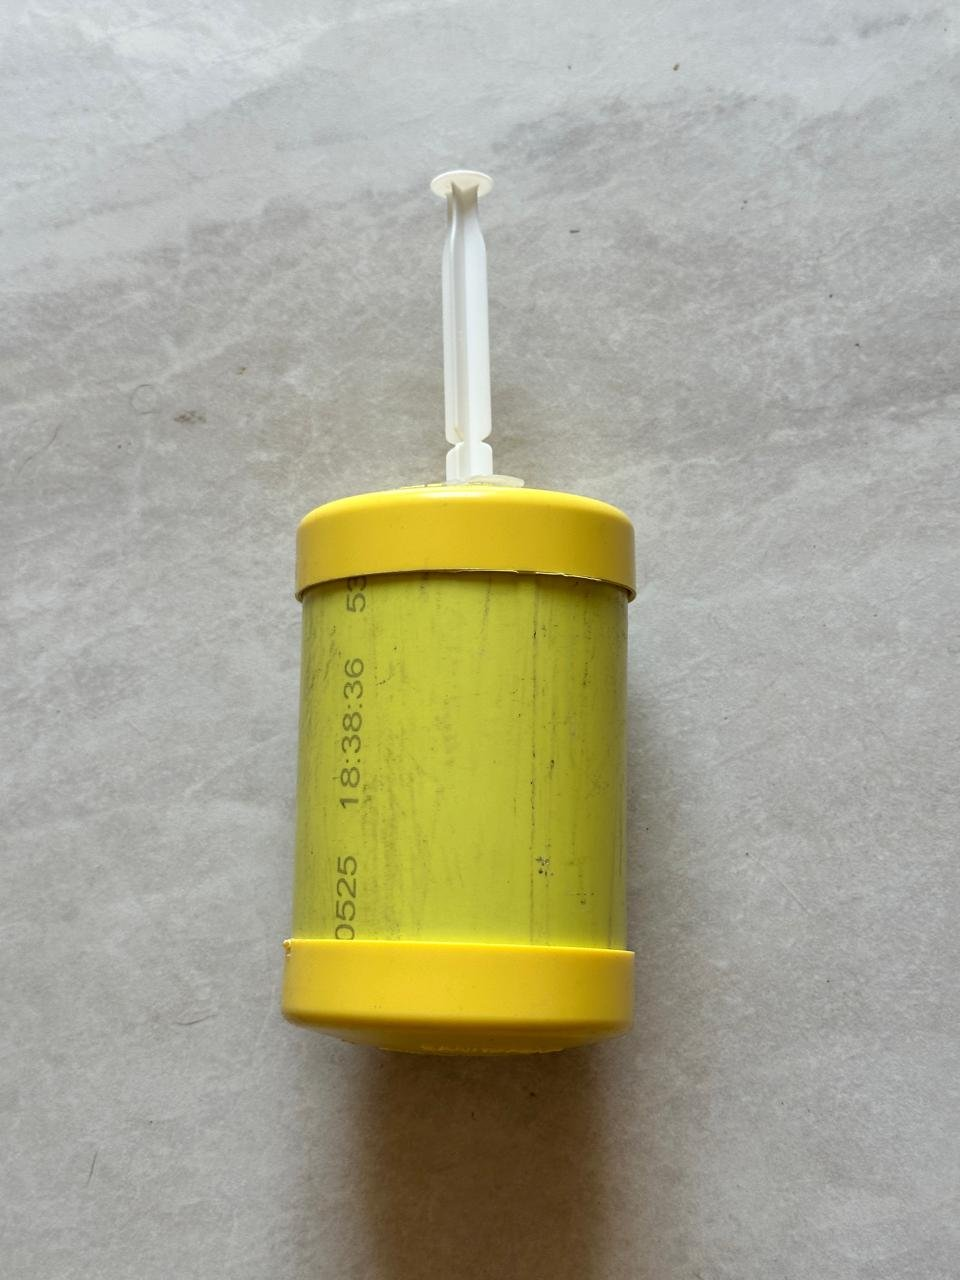
\includegraphics[height=6cm]{figuras/mina_lateral.png}
    \caption{Vista lateral}
  \end{subfigure}
  \hspace{1cm}
  \begin{subfigure}[b]{0.40\textwidth}
    \centering
    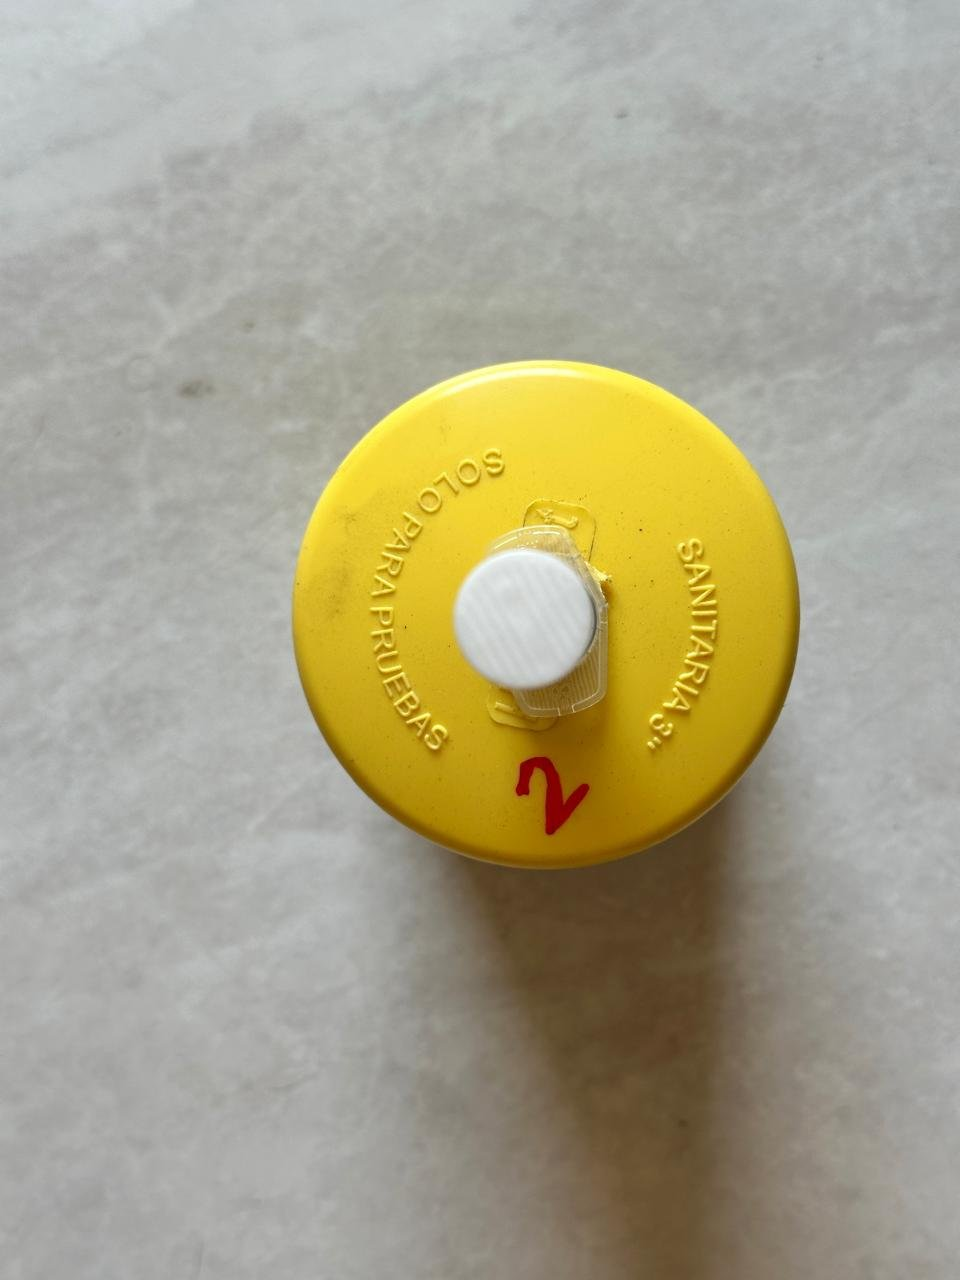
\includegraphics[height=6cm]{figuras/mina_superior.png}
    \caption{Vista superior (tapa con cabeza de émbolo expuesta)}
  \end{subfigure}
  \caption{Mina emulada tipo quiebrapatas construida para el experimento.
           Cilindro de \ac{PVC} con carbón de antracita, clavos y pila de 9~V
           en su interior. La cabeza del émbolo de la jeringa queda expuesta
           sobre la superficie del suelo; en la base de datos definitiva se cubre
           con hojas del entorno para evitar su detección trivial.}
  \label{fig:minas_simuladas}

  {\footnotesize Fuente: elaboración propia.}
\end{figure}

\subsection{Objetos de interferencia (potenciales falsos positivos)}
\label{sec:objetos_interferencia}

Con el propósito de dotar al experimento de mayor realismo, en cada zona de
mina se dispusieron tres objetos de interferencia \textbf{enterrados a la
misma profundidad que la mina correspondiente}, a \SI{20}{cm} de distancia
del centro: una roca a la izquierda, una botella de vidrio en la parte
superior y una lata de aluminio a la derecha. Esta distribución se mantuvo
constante en todas las zonas  con mina y sesiones (véase Figura~\ref{fig:disposicion_zona}).

Cada zona de captura cubre un área de aproximadamente \SI{60}{cm} $\times$
\SI{60}{cm}, con la mina ubicada en el centro geométrico de la subárea.
Los objetos de interferencia quedan a los lados, dentro del campo de visión
de la cámara pero fuera de la región central donde se concentra la firma
espectral de la mina.

La selección de estos objetos responde a dos criterios. Primero, todos ellos
aparecen en contextos reales de terrenos minados: rocas y objetos metálicos
son comunes en zonas rurales colombianas. Segundo, y más importante para el
diseño experimental, cada objeto puede generar anomalías espectrales que
el clasificador podría confundir con una \ac{MAP}:

\begin{itemize}
  \item \textbf{Roca:} su composición mineralógica diferente al suelo circundante
    genera una firma espectral distinta en las bandas Roja y Red Edge,
    potencialmente similar a la perturbación del suelo sobre una mina.
  \item \textbf{Botella de vidrio:} su alta reflectancia en el espectro visible
    genera valores anómalos en índices como \ac{VARI} y \ac{NDRB},
    similares a los producidos por suelo perturbado.
  \item \textbf{Lata de aluminio:} los metales tienen reflectancia muy alta y
    relativamente plana en todas las bandas, generando valores atípicos en
    índices que involucran ratios entre bandas visibles e infrarrojas.
\end{itemize}

El análisis de qué fracción de los falsos positivos se asocia a estos
objetos se presenta en la Sección~\ref{sec:analisis_fp}.

\begin{figure}[H]
  \centering
  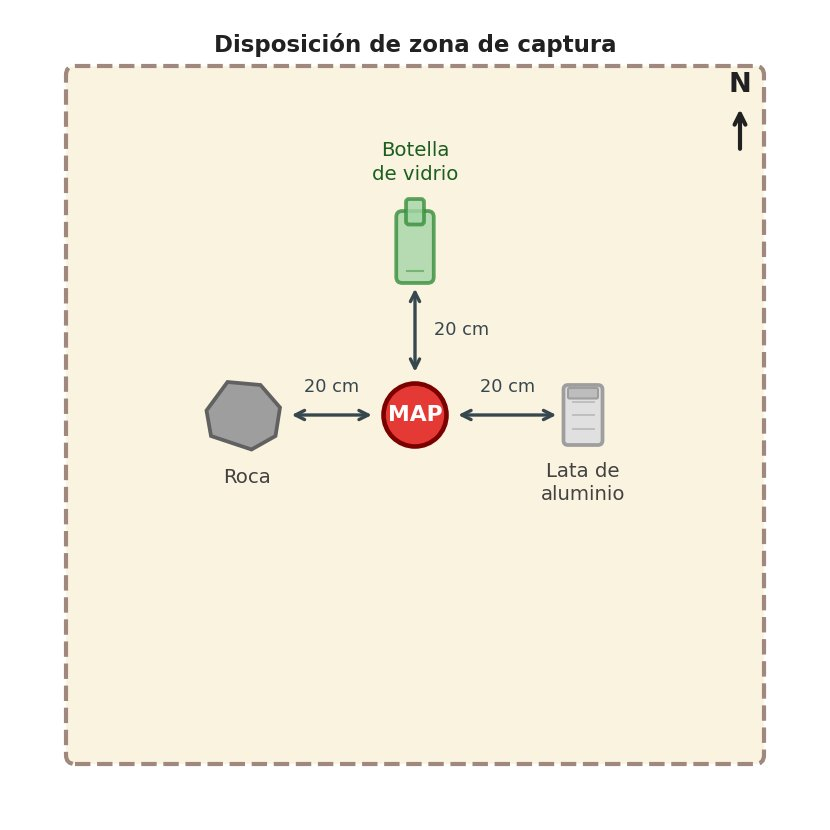
\includegraphics[width=0.45\textwidth]{figuras/disposicion_zona.png}
  \caption{Esquema de disposición de la mina emulada y los objetos de
           interferencia en cada zona de captura (\SI{60}{cm} $\times$ \SI{60}{cm}).
           La \ac{MAP} se ubica en el centro; la roca a la izquierda, la
           botella de vidrio en la parte superior y la lata de aluminio a
           la derecha, todos enterrados a la misma profundidad que la mina
           y a \SI{20}{cm} del centro.}
  \label{fig:disposicion_zona}

  {\footnotesize Fuente: elaboración propia.}
\end{figure}


\subsection{Descripción del terreno experimental}

El experimento se llevó a cabo en un área verde del campus de la Universidad
del Valle, sede Meléndez, en Santiago de Cali. El terreno seleccionado
presenta suelo con predominio de textura arenosa y vegetación limitada,
compuesta principalmente por gramíneas y plantas herbáceas de hoja ancha. La zona está rodeada por árboles de mediano y gran porte y
tiene una edificación adyacente, lo que genera condiciones de sombra
parcial en horas de la mañana temprana.

El área total del terreno experimental es de aproximadamente
\textbf{\SI{10}{m} $\times$ \SI{6}{m}}. La Figura~\ref{fig:terreno} muestra
el área de trabajo: la vista general antes del experimento y la disposición
de las zonas delimitadas con cinta de señalización amarilla durante una
sesión de campo.

\begin{figure}[H]
  \centering
  \begin{subfigure}[b]{0.48\textwidth}
    \centering
    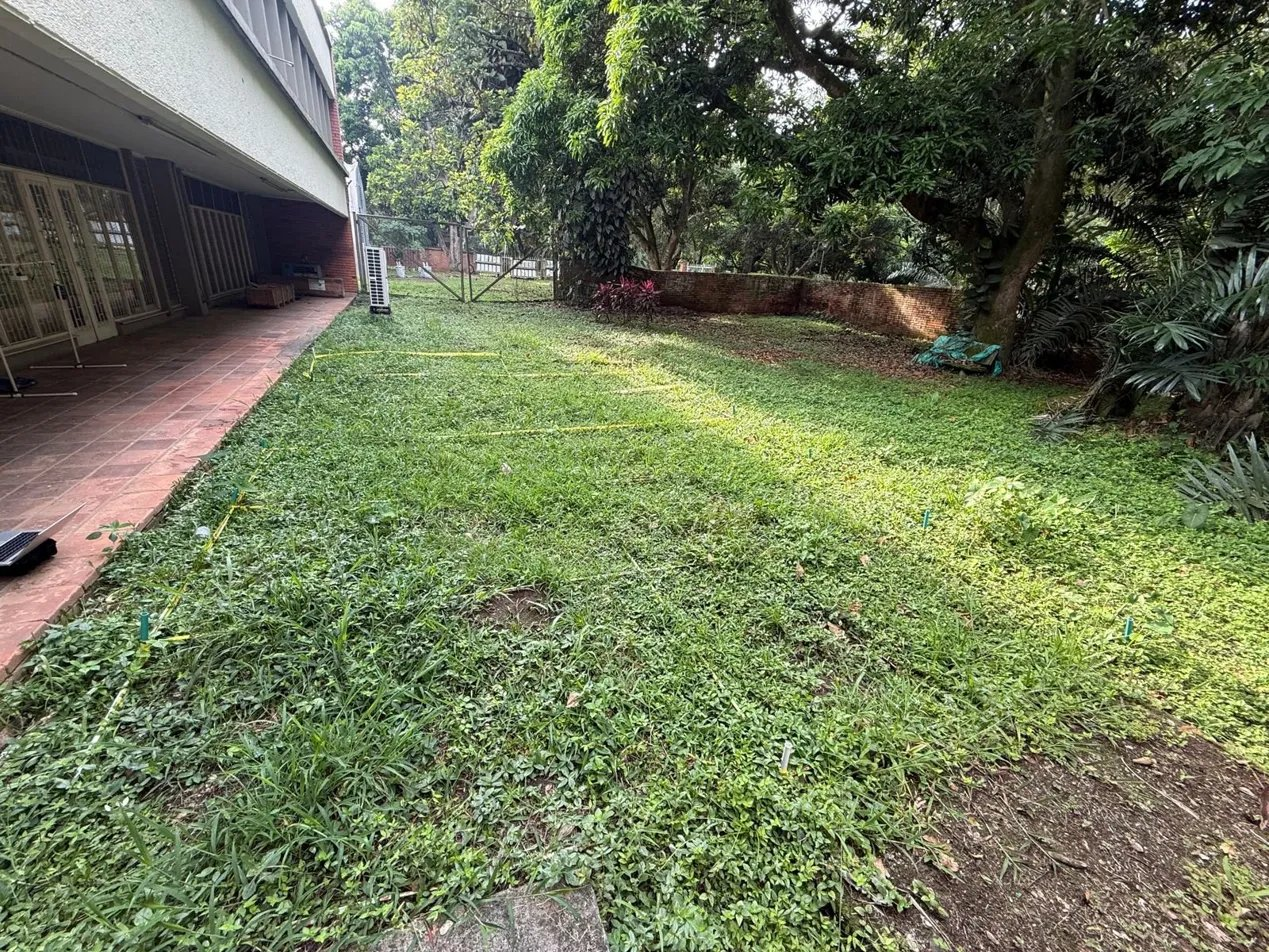
\includegraphics[width=\textwidth]{figuras/terreno_general.png}
    \caption{Vista general del área experimental}
  \end{subfigure}
  \hfill
  \begin{subfigure}[b]{0.48\textwidth}
    \centering
    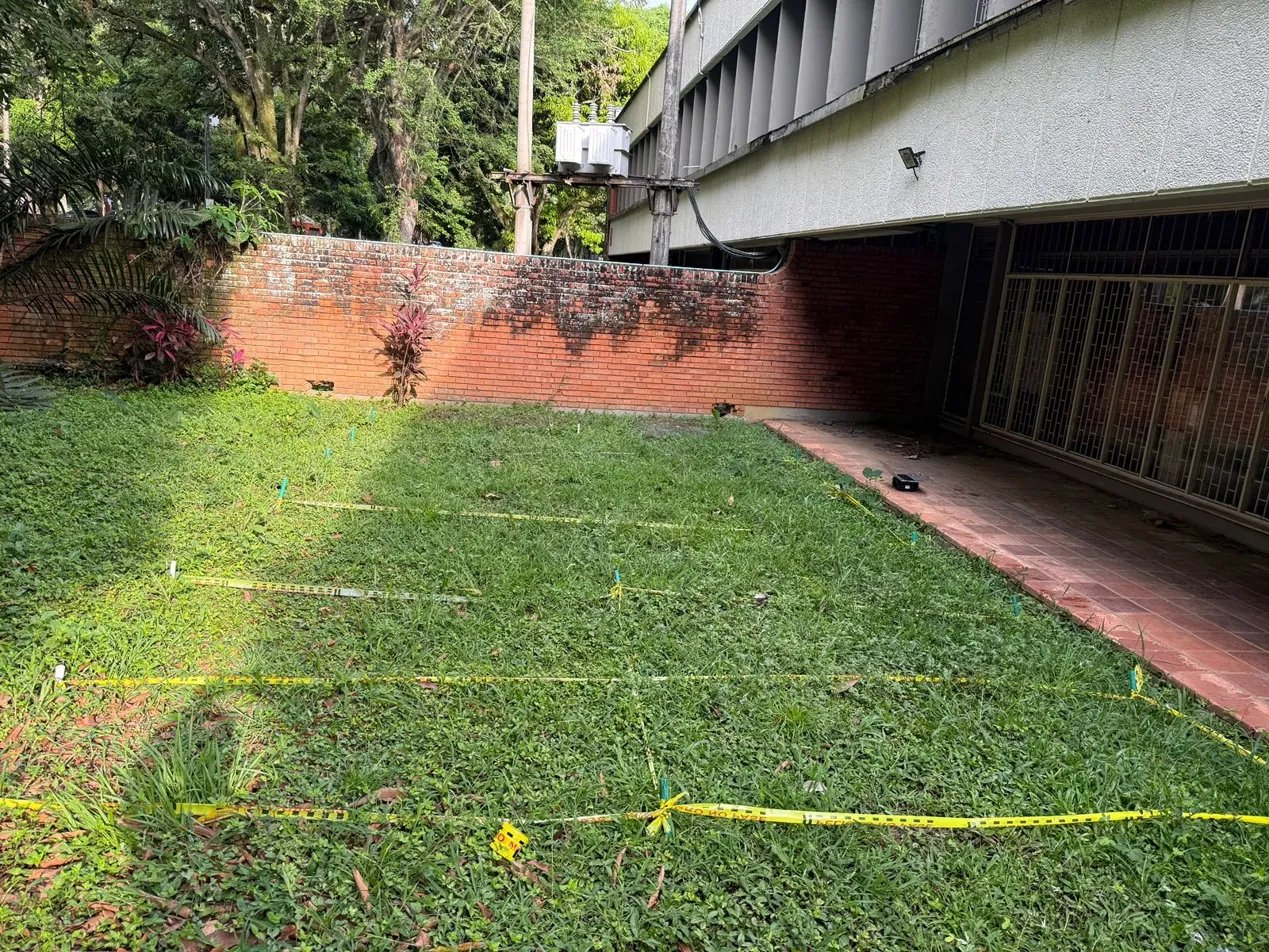
\includegraphics[width=\textwidth]{figuras/terreno_delimitado.png}
    \caption{Zonas delimitadas con cinta de señalización}
  \end{subfigure}
  \caption{Terreno experimental en el campus de la Universidad del Valle,
           sede Meléndez. (a) Vista general con cobertura vegetal limitada, rodeada por árboles de mediano y gran porte y una
           edificación adyacente. (b) Distribución de las doce zonas de
           captura delimitadas con estacas y cinta amarilla.}
  \label{fig:terreno}

  {\footnotesize Fuente: elaboración propia.}
\end{figure}

Previo al inicio del experimento se realizó una poda completa de la
vegetación en toda el área de trabajo con el propósito de homogenizar
las condiciones iniciales y garantizar vegetación limitada, en concordancia
con el objetivo específico~1 del presente trabajo. A partir de ese momento
no se realizó ninguna intervención adicional, permitiendo el crecimiento
natural de la vegetación durante todo el período experimental. Las minas
llevan aproximadamente seis meses enterradas desde el inicio del
experimento, tiempo suficiente para que los efectos crónicos del
enterramiento ---perturbación del suelo y posible estrés vegetal
diferencial--- se hayan desarrollado progresivamente. Un aspecto favorable
de este diseño es que la vegetación cubre completamente las zonas de mina,
haciendo que los artefactos sean invisibles a simple vista, simulando
fielmente el camuflaje natural de las \ac{MAP} en entornos reales.

Para garantizar la altura y verticalidad de la captura con precisión y
reproducibilidad entre sesiones, se diseñó e implementó una estructura de
soporte fabricada en tubo de \ac{PVC} que posiciona la cámara a exactamente
\SI{1}{m} sobre cada zona (véase Sección~\ref{sec:montaje}). Esta solución
podría ser reemplazada en trabajos futuros por un \ac{UAV} volando a dicha
altura, lo que permitiría escalar el sistema a áreas de mayor extensión.



\subsection{Distribución de zonas}

El área experimental de \SI{10}{m} $\times$ \SI{6}{m} se subdividió en
doce zonas de captura distribuidas en una matriz de $6 \times 2$, como
se muestra en la Figura~\ref{fig:distribucion_zonas}.

\begin{figure}[H]
  \centering
  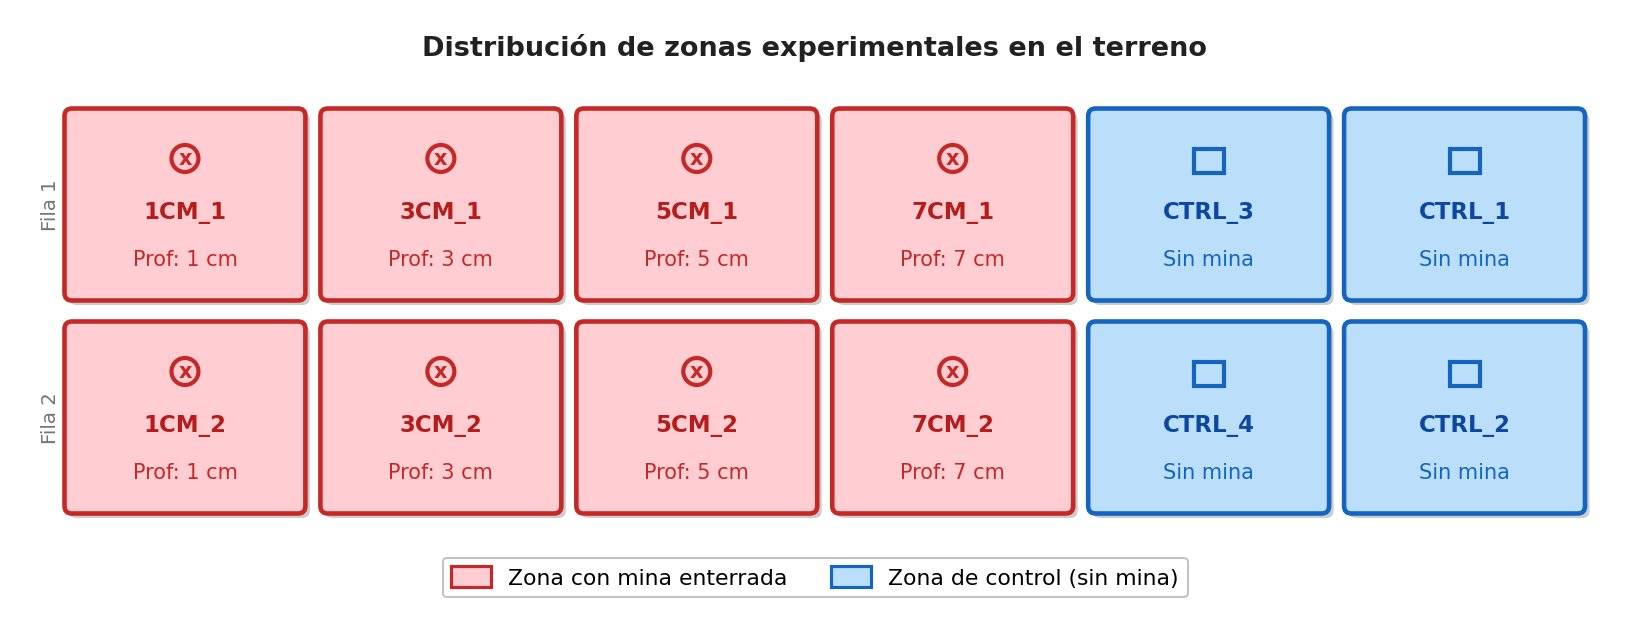
\includegraphics[width=0.95\textwidth]{figuras/distribucion_zonas.png}
  \caption{Distribución de las doce zonas de captura en el área experimental
         de \SI{10}{m} $\times$ \SI{6}{m}, organizadas en una matriz de
         $6 \times 2$. Cada zona cubre \SI{60}{cm} $\times$ \SI{60}{cm},
         con la \ac{MAP} emulada ubicada en el centro geométrico. Las zonas
         rojas contienen \ac{MAP} enterradas a distintas profundidades; las
         azules son de control (sin mina). Cada zona de mina incluye además
         tres objetos de interferencia enterrados a la misma profundidad
         (véase Sección~\ref{sec:objetos_interferencia}).}
  \label{fig:distribucion_zonas}

  {\footnotesize Fuente: elaboración propia.}
\end{figure}

Cada zona fue delimitada con estacas y cinta de señalización amarilla
para garantizar la reproducibilidad de la posición de captura entre sesiones.
A partir de la Sesión~3 se incorporaron cuatro zonas de control por sesión
(relación 2:1 respecto a las zonas de mina), frente a la única zona de control
de la Sesión~2 (relación 8:1), con el fin de reducir el desbalance de clases
en el conjunto de entrenamiento.



\subsection{Iteración previa del diseño experimental}
\label{sec:iteracion_previa}

Antes de constituir la base de datos definitiva, se realizó una fase experimental
previa que fue descartada en su totalidad. En esa iteración, las minas
emuladas se enterraban dejando la cabeza del émbolo de la jeringa completamente blanco expuesta
sobre la superficie del terreno durante las capturas, sin cubrirla. Este
elemento de color blanco intenso generaba una firma espectral trivialmente
discriminable: algoritmos de segmentación básicos como k-means identificaban
la zona de la mina con casi el 100\,\% de exactitud, no por detectar la
perturbación del suelo o el estrés vegetal asociados a la mina enterrada,
sino por detectar el color blanco del émbolo en la imagen de espectro visible.

La detección del émbolo visible no constituye una solución al problema
planteado --- en una situación real, las \ac{MAP} probablemente no presentarían elementos
tan contrastantes en superficie --- por lo que se tomó la decisión de reiniciar
la base de datos completa, cubriendo los émbolos con hojas u otro material vegetal
del entorno antes de cada captura, de modo que las minas emuladas no tuvieran
ningún elemento visible que facilitara su localización trivial. Esta decisión
está alineada con el objetivo de detectar anomalías espectrales sutiles del
suelo y la vegetación, no elementos superficiales de alta reflectancia.

Las imágenes de la iteración previa se conservan como registro, pero no
se utilizan en ninguna etapa del análisis presentado en este trabajo.

% -------------------------------------------------------------
\section{Protocolo de adquisición de imágenes}

\subsection{Sistema de soporte de la cámara}
\label{sec:montaje}

Para garantizar la altura de captura con precisión y reproducibilidad entre
sesiones, se diseñó y construyó un sistema de soporte estacionario fabricado
en tubo de \ac{PVC}, con forma de pórtico en H, que posiciona la cámara a
exactamente \SI{1}{m} sobre cada zona de captura
(véase Figura~\ref{fig:soporte}). Esta solución permitió controlar con
precisión la altura y la verticalidad de la cámara, condiciones difíciles
de garantizar en vuelo libre. En el futuro, la misma metodología podría
aplicarse montando la cámara en un \ac{UAV} volando a dicha altura, lo
que permitiría escalar el sistema a áreas de mayor extensión.

% \begin{figure}[H]
%   \centering
%   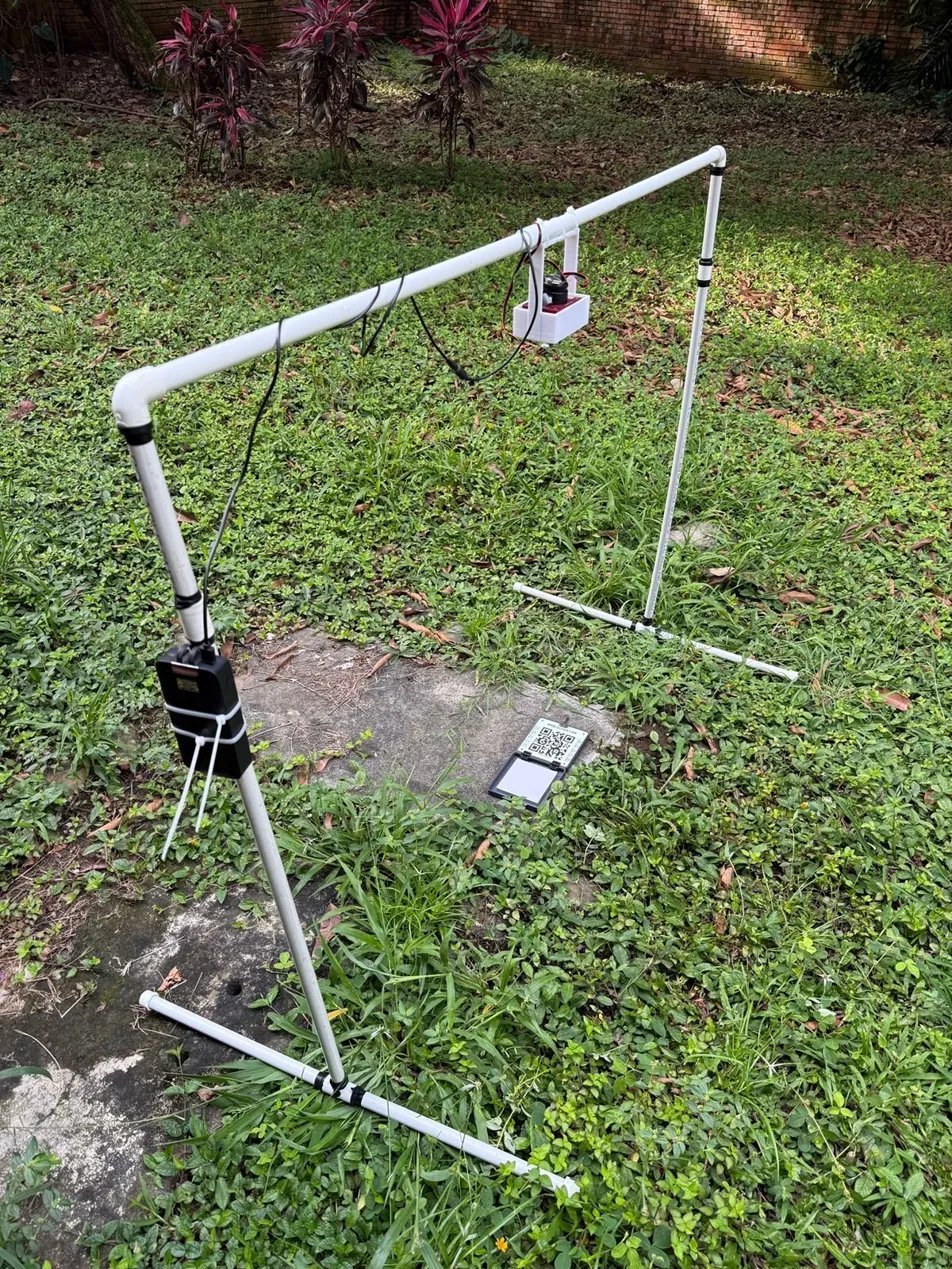
\includegraphics[width=0.7\textwidth]{figuras/soporte_pvc.jpg}
%   \caption{Sistema de soporte de la cámara MicaSense RedEdge-MX.
%            Estructura de tubo PVC con soporte impreso en 3D (color morado)
%            para fijar la cámara en posición nadir a \SI{1}{m} de altura.}
%   \label{fig:soporte}
% \end{figure}

La cámara MicaSense RedEdge-MX se fija en el extremo horizontal del pórtico
mediante un soporte fabricado en impresión 3D, apuntando en posición nadir
(perpendicular al suelo). La Figura~\ref{fig:soporte} muestra el sistema completo
durante una sesión de campo, con el panel de calibración de reflectancia
visible en el suelo. La altura se verificó con un metro desde el nivel
del suelo hasta los lentes de la cámara, con un margen de error de
$\pm$\SI{3}{cm}. La verticalidad del soporte se comprobó con un nivel de
burbuja antes de cada captura. La estructura se desplazó manualmente de zona
en zona, reposicionándose sobre el centro de cada área delimitada.

\begin{figure}[H]
  \centering
  \begin{subfigure}[b]{0.52\textwidth}
    \centering
    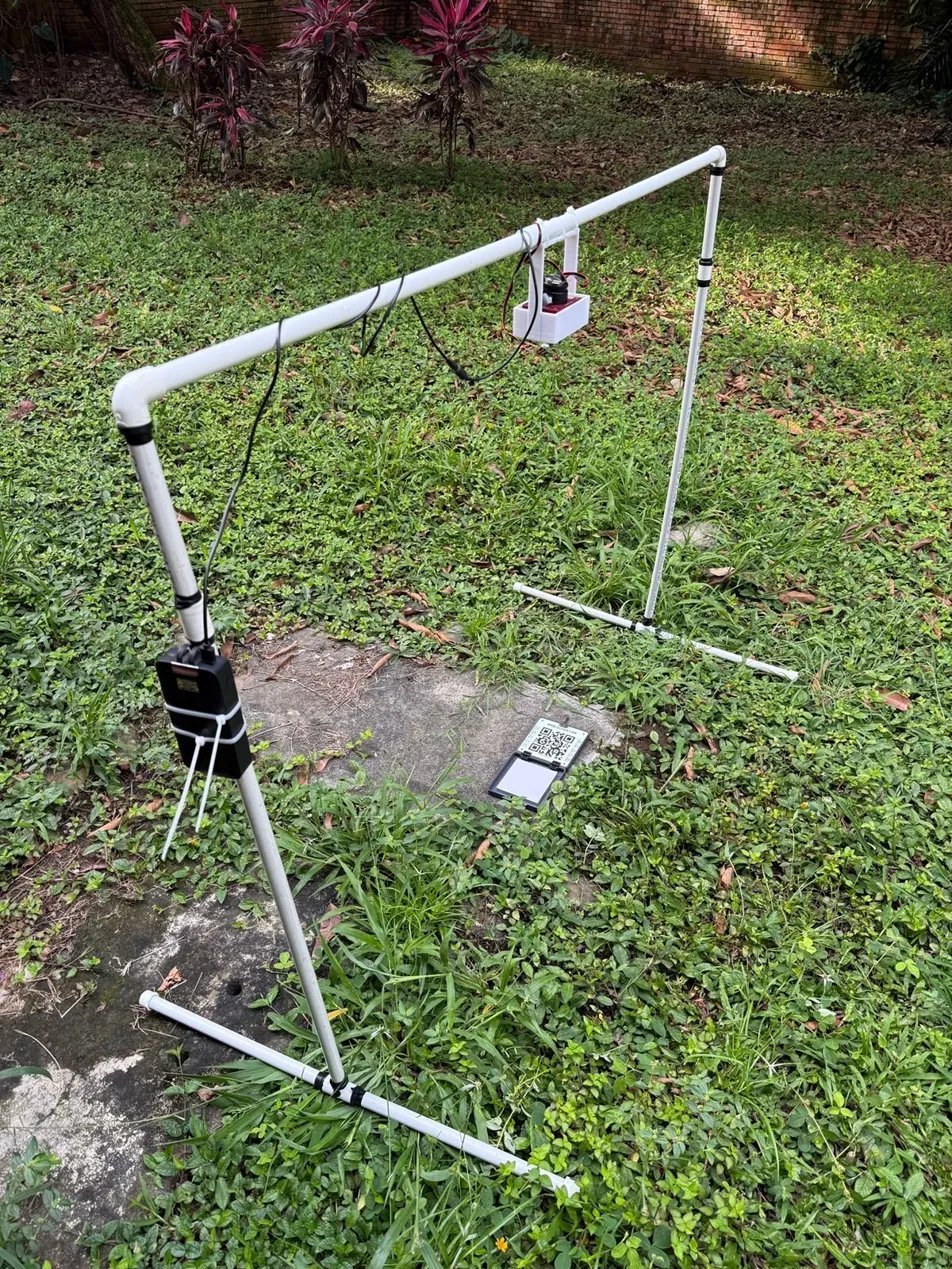
\includegraphics[width=\textwidth]{figuras/soporte_pvc.png}
    \caption{Sistema de soporte en pórtico de \ac{PVC} con la cámara
             en posición nadir. El panel \ac{CRP} se observa en el suelo.}
  \end{subfigure}
  \hfill
  \begin{subfigure}[b]{0.42\textwidth}
    \centering
    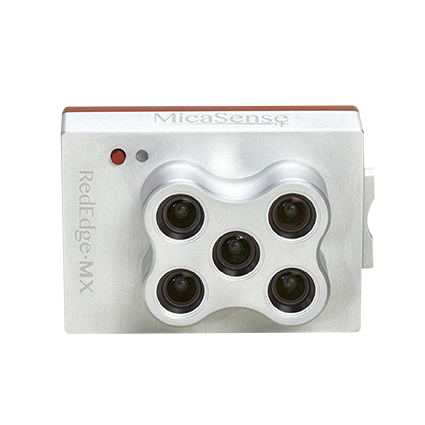
\includegraphics[width=\textwidth]{figuras/micasense_rededge.png}
    \caption{Cámara MicaSense RedEdge-MX con sus cinco lentes
             correspondientes a las bandas Blue, Green, Red,
             Red Edge y NIR.}
  \end{subfigure}
  \caption{Equipo de captura multiespectral utilizado en el experimento.}
  \label{fig:soporte}

  {\footnotesize Fuente: (a) elaboración propia; (b) tomado de \url{https://al-top.com/producto/micasense-rededge-mx/}.}
\end{figure}

La elección de un sistema estacionario, aunque limita la movilidad en
comparación con un \ac{UAV}, ofrece ventajas para este experimento: permite
tiempos de captura más largos por zona, elimina la inestabilidad posicional
causada por el viento que afecta a los drones a baja altura, y garantiza
una altura de adquisición más consistente.

\subsection{Condiciones ambientales}

Las condiciones meteorológicas durante cada sesión de campo se registraron
a partir de la estación meteorológica de la Universidad del Valle, ubicada
en las proximidades del área de experimentación. Las variables registradas
fueron: irradiancia solar global (\si{W/m^2}), temperatura del aire
(\si{\celsius}), humedad relativa (\%), precipitación acumulada en las
24~horas previas (\si{mm}) y cobertura nubosa estimada. La
Tabla~\ref{tab:condiciones_ambientales} resume estas condiciones para cada
sesión de captura.

\begin{table}[H]
\centering
\caption{Condiciones ambientales registradas por sesión de captura}
\label{tab:condiciones_ambientales}
\begin{tabular}{ccccccc}
\toprule
\textbf{Sesión} & \textbf{Fecha} & \textbf{Hora} & \textbf{Rad. solar (\si{W/m^2})} &
\textbf{Temp. (\si{\celsius})} & \textbf{HR (\%)} & \textbf{Precip. 24h (\si{mm})} \\
\midrule
S1            & 16 abr. & 09:44 & 620.0 & 22.4 & 90.5 & 8.0 \\
S2            & 16 abr. & 13:10 & 778.7 & 26.4 & 72.8 & 5.2 \\
S3            & 23 abr. & 12:34 & 346.7 & 28.2 & 60.7 & 0.0 \\
S4            & 24 abr. & 17:21 &  64.5 & 27.5 & 61.8 & 0.0 \\
S5            & 30 abr. & 17:17 &  73.3 & 29.2 & 63.6 & 0.0 \\
S6            & 07 may. & 07:30 & 161.5 & 23.6 & 84.5 & 0.0 \\
S7            & 07 may. & 16:40 & 143.9 & 29.1 & 65.5 & 0.0 \\
\bottomrule
\multicolumn{7}{l}{\small Todas las sesiones en 2026. S6 y S7 fueron capturadas el mismo día en horarios distintos.} \\
\multicolumn{7}{l}{\small S1: HR=90.5\,\% y precipitación previa de 8.0~mm; no forma parte de la base de datos oficial (S2--S7).}
\end{tabular}

  {\footnotesize Fuente: elaboración propia.}
\end{table}

Las condiciones ambientales registradas evidencian la variabilidad presente
en la base de datos. La Sesión~2 fue capturada a las 13:10 con HR~=~72.8\,\%
y precipitación previa de 5.2~mm. Las sesiones S3 a S5 registraron
HR~$\approx$~61\,\% y precipitación nula en las 24~h previas. La Sesión~6
fue capturada a las 07:30 con HR~=~84.5\,\% y ángulo solar rasante. La base
de datos oficial comprende las sesiones S2--S7; la Sesión~1 se excluyó de
ella. Sus condiciones atípicas ---captura a las 09:44 con posible rocío
(HR~=~90.5\,\%, precipitación previa de 8.0~mm) y una sola zona de control
disponible--- degradaron la señal hasta un AUC~$\approx$~0.47 como fold de
prueba, por debajo del nivel de azar. Más que un dato descartable, la
Sesión~1 establece empíricamente un \textbf{límite operativo} del enfoque: la
alta humedad superficial satura la respuesta espectral pasiva. Por ello se
excluye del protocolo oficial (S2--S7) y se retoma como limitación en el
Capítulo~\ref{cap:conclusiones}.

\subsection{Procedimiento de captura}

Para cada sesión de campo, el procedimiento de captura siguió los pasos:

\begin{enumerate}
\item \textbf{Captura del panel de calibración al inicio.} Antes de
  recorrer las zonas, se capturó una imagen del Panel de Reflectancia
  Calibrada (\ac{CRP}) bajo iluminación directa de sol, con la cámara
  apuntando en posición nadir (perpendicular al suelo, apuntando
  verticalmente hacia abajo) sobre el panel dispuesto horizontalmente
  en el suelo, en un área adyacente a la matriz experimental
  (Figura~\ref{fig:panel_crp}).

\begin{figure}[H]
  \centering
  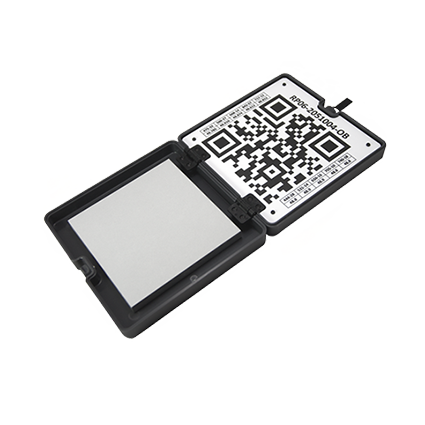
\includegraphics[width=0.40\textwidth]{figuras/panel_crp.png}
  \caption{Panel de Reflectancia Calibrada (\ac{CRP}) de MicaSense
           utilizado para la calibración radiométrica. Sus valores de
           albedo conocidos (Blue: 0.490, Green: 0.491, Red: 0.491,
           Red Edge: 0.488, NIR: 0.490) permiten convertir los valores
           digitales de cada banda a reflectancia absoluta.}
  \label{fig:panel_crp}

  {\footnotesize Fuente: tomado de \url{https://www.airclip.de/MicaSense-Calibrated-Reflectance-Panel-V2}.}
\end{figure}

  \item \textbf{Captura por zona.} El soporte de \ac{PVC} se posicionó sobre
    el centro de cada zona, se verificó la altura y la verticalidad
    mediante nivel de burbuja, y se capturaron las cinco bandas
    simultáneamente. El recorrido siguió un orden fijo de derecha a
    izquierda en zigzag: primero las zonas de control
    (CTRL\_1, CTRL\_2, CTRL\_3, CTRL\_4) y luego las zonas de mina en
    orden decreciente de profundidad (7CM\_1, 7CM\_2, 5CM\_1, 5CM\_2,
    3CM\_1, 3CM\_2, 1CM\_1, 1CM\_2), repitiéndose idéntico en cada sesión.
  \item \textbf{Criterio de iluminación uniforme.} Antes de capturar cada
    zona se verificó que toda el área estuviera bajo la misma condición de luz
    —completamente iluminada o completamente en sombra—, evitando capturas
    con sombras parciales que introducirían gradientes espectrales
    artificiales. Las sombras proyectadas por el edificio adyacente en
    determinadas horas constituían el principal riesgo de incumplimiento
    de este criterio; por ello fue un factor considerado en la selección
    del horario de captura.
  \item \textbf{Captura del Panel de Reflectancia Calibrada al final.}
  Al concluir el recorrido de todas las zonas se repite la captura del
  Panel de Reflectancia Calibrada (\ac{CRP}), para verificar que las
  condiciones de iluminación se mantuvieron estables durante toda la
  sesión y para detectar posibles cambios en las condiciones de iluminación
  comparando los valores de reflectancia del panel al inicio y al final de
  la sesión.
\end{enumerate}

\textbf{Criterio de horario.} Las sesiones S2--S7 se capturaron en distintas
franjas horarias ---mediodía, tarde y mañana temprana--- para
evaluar la estabilidad del sistema ante variaciones de iluminación. El
criterio mínimo aplicado fue evitar capturas con humedad muy alta o
precipitación reciente: la Sesión~1, realizada a las 09:44 con
HR~=~90.5\,\% y precipitación previa de 8.0~mm, produjo firmas espectrales
que se apartaron significativamente del patrón del resto de sesiones, lo que
motivó su exclusión de la base de datos oficial.

\subsection{Estructura de archivos}

Cada captura genera cinco archivos TIFF (uno por banda), nombrados
\texttt{cap\_0001\_band1.tif} a \texttt{cap\_0001\_band5.tif}, organizados
según la siguiente jerarquía:

\begin{lstlisting}[language=bash, caption={Estructura del conjunto de datos}, label={lst:estructura}]
FINAL_DATASET/
+-- SESION_N/
|   +-- PANEL_INICIO/        # 5 TIF (panel al inicio)
|   +-- MINA_1CM_1/          # 5 TIF por zona
|   +-- MINA_3CM_1/ ...
|   +-- ZONA_CONTROL/ ...
|   +-- PANEL_FINAL/         # 5 TIF (panel al final)
|   +-- PROCESADAS/          # generado por el pipeline
|       +-- *_calibrado.tif
|       +-- features_dataset.csv
+-- features_combinado.csv   # todas las sesiones combinadas
\end{lstlisting}

% -------------------------------------------------------------
\section{Etapa 1: Preprocesamiento}

El preprocesamiento consta de tres pasos: calibración radiométrica, alineación entre bandas y recorte
de bordes.

\subsection{Calibración radiométrica}

La calibración radiométrica convierte los valores digitales crudos (DN) capturados
por el sensor en reflectancia de superficie, eliminando la dependencia de las
condiciones de iluminación entre sesiones \cite{daniels2023}. Para cada sesión
se detecta la máscara del \ac{CRP} en la banda Roja (banda 3), que presenta el
mayor contraste entre el panel y el fondo en este rango espectral. Dicha máscara
se aplica a las cinco bandas para extraer los valores de DN correspondientes al
panel. Con esos valores se aplica la siguiente ecuación (véase
Sección~\ref{sec:calibracion_teorica} para la derivación completa):
\begin{equation*}
  \rho_{\text{sup}}(\lambda) =
  \frac{\text{DN}_{\text{zona}}(\lambda)}{\text{DN}_{\text{panel}}(\lambda)}
  \cdot \rho_{\text{panel}}(\lambda)
\end{equation*}
donde $\rho_{\text{panel}}(\lambda)$ es la reflectancia nominal del panel
para la banda $\lambda$.

\textbf{Decisión técnica clave.} La detección del panel se realiza únicamente
sobre la banda Roja porque en la banda Red Edge (banda 4), la vegetación
circundante y el panel tienen reflectancias similares (\textasciitilde717~nm),
lo que hace que el método de umbralización de Otsu detecte erróneamente
el 57\,\% de la imagen como panel. Al compartir la máscara de la banda Roja
entre todas las bandas, la irradiancia estimada de la banda Red Edge mejoró de
191\,222 a 197\,502 y el \ac{NDRE} pasó de $-0.318$ a $-0.151$
.

\subsection{Alineación de bandas}

La alineación corrige el desalineamiento geométrico entre las cinco bandas,
causado por el paralaje entre los lentes físicamente separados de la MicaSense
a \SI{1}{m} de altura (véase Sección~\ref{sec:alineacion}). Se utiliza la banda
Roja como imagen de referencia y las cuatro bandas restantes se alinean sobre ella.

El algoritmo \ac{SIFT} \cite{sift_lowe2004} extrae puntos clave
(\textit{keypoints}) con sus descriptores locales en ambas imágenes: son
regiones distintivas invariantes a cambios de escala, rotación e iluminación.
Los puntos clave se emparejan por similitud de descriptores y se estima una
homografía global (transformación de perspectiva de 8 parámetros) mediante
RANSAC: el algoritmo selecciona muestras aleatorias de cuatro pares de puntos,
calcula la homografía candidata y conserva la que maximiza el número de pares
consistentes con esa transformación (\textit{inliers}). Si \ac{SIFT} genera
menos de cuatro inliers tras el filtrado ---condición que ocurre en imágenes
con textura muy uniforme--- se recurre al algoritmo ECC
(\textit{Enhanced Correlation Coefficient}), que estima la misma transformación
por optimización iterativa de la correlación entre imágenes y es más robusto
en esas condiciones, a costa de mayor tiempo de cómputo.

\subsection{Recorte de bordes}

El recorte de bordes elimina las franjas de píxeles con valor cero
(\textit{zero-padding}) que introduce la homografía en los bordes de la imagen
transformada, evitando que esas regiones vacías contaminen la extracción de
características.

Los valores de recorte se determinaron empíricamente inspeccionando las imágenes
alineadas de todas las sesiones: se buscó el recorte mínimo que elimina todas
las franjas de ceros en la totalidad de las capturas, minimizando la pérdida de
información útil:

\begin{equation}
  \text{Recorte} = \{\text{top}: 20, \text{bottom}: 60, \text{left}: 35, \text{right}: 20\}\ \text{píxeles}
  \label{eq:crop}
\end{equation}

Los valores mayores en el margen inferior e izquierdo obedecen a que el
\textit{zero-padding} del \textit{warpPerspective} se concentra en esas
direcciones. La imagen resultante tiene dimensiones aproximadas de
1185$\times$840 píxeles.

% -------------------------------------------------------------
\section{Etapa 2: Extracción de características}

\subsection{Búsqueda de la mina mediante ventanas deslizantes}
\label{sec:extraccion_parches}

A diferencia de métodos de segmentación explícita (umbralización, crecimiento
de regiones), aquí no se delimita la región de la mina de forma previa: el
clasificador aprende a distinguir ventanas con MAP de ventanas sin MAP
directamente a partir de los valores de las características extraídas. Este
enfoque es adoptado en los trabajos de referencia del campo
\cite{clark2000, silva2019} y se justifica por las siguientes razones:

\begin{enumerate}
  \item \textbf{Señal espectral débil con base de datos pequeño.} Los métodos de
    segmentación basados en umbralización o regiones (Otsu, watershed, k-means)
    requieren un contraste espectral pronunciado entre el objeto y el fondo.
    Con la señal multiespectral de una \ac{MAP} enterrada ---que es sutil e
    indirecta--- estos métodos generarían un número elevado de falsos positivos
    sin poder aprender de los datos de entrenamiento.

  \item \textbf{Aprovechamiento del contexto espectral.} El tamaño de
    $128\times128$ píxeles fue elegido para que cada ventana
    sea mayor que la mina, capturando tanto la zona directamente sobre el
    artefacto como el suelo circundante. Esta información de contexto permite
    al clasificador detectar la anomalía espectral relativa, algo que una
    segmentación basada únicamente en el valor absoluto del píxel no podría
    aprovechar.

  \item \textbf{Compatibilidad con el esquema de etiquetado.} Las imágenes
    fueron capturadas por zona (una imagen completa por zona de mina o control),
    por lo que la etiqueta de cada ventana se hereda directamente de la zona de
    origen. Esto hace que el enfoque por ventanas sea la estrategia de
    segmentación natural para este diseño experimental.
\end{enumerate}

La búsqueda se realiza con una ventana de $128\times128$ píxeles y solapamiento
del 50\,\%. El solapamiento garantiza que zonas de mina próximas al borde de
una ventana queden capturadas en la ventana vecina, y duplica el número de
muestras respecto a ventanas sin solapamiento: para una imagen de
$1185\times840$ píxeles se generan aproximadamente 216 ventanas, lo que hace
viable el entrenamiento con el conjunto de datos disponible. Cada ventana
define una región sobre la cual se calculan las características espectrales y
estadísticas; sus valores son los que el clasificador usa para determinar si
esa región contiene o no una \ac{MAP}
(Figura~\ref{fig:ventanas_solapamiento}).

\begin{figure}[H]
  \centering
  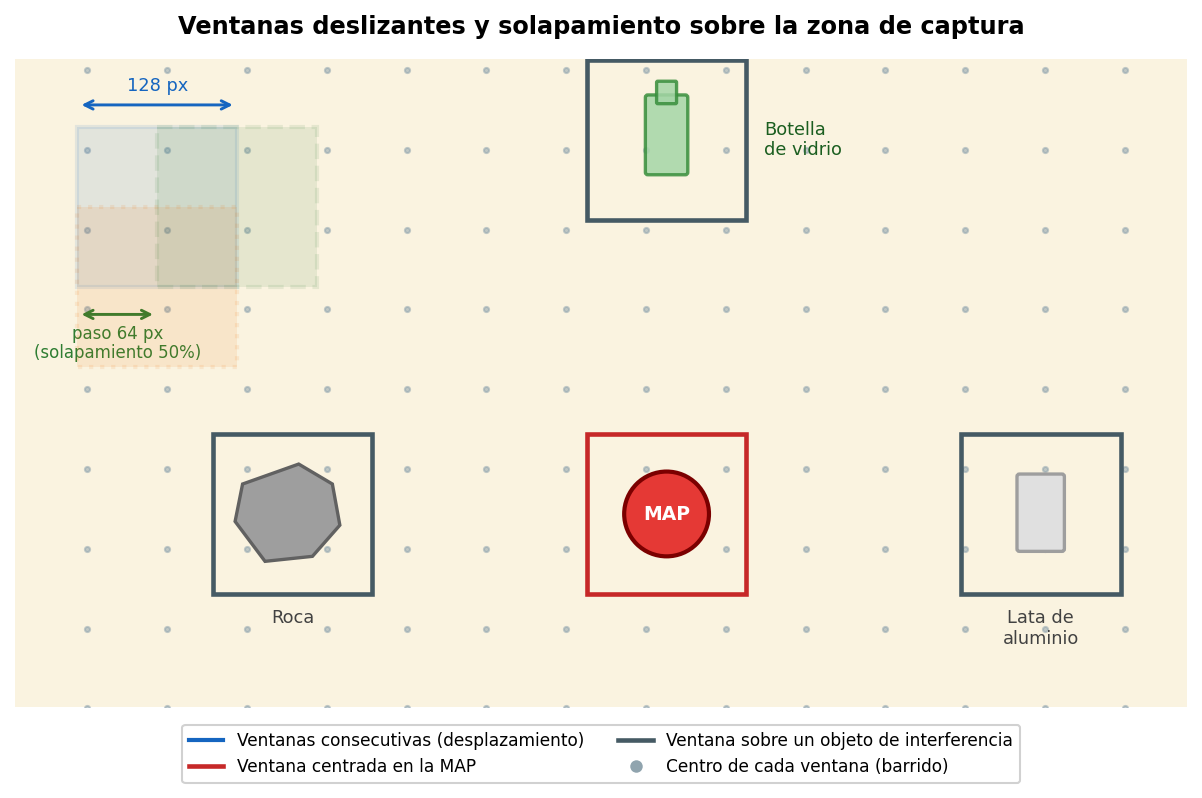
\includegraphics[width=0.92\textwidth]{figuras/ventanas_solapamiento.png}
  \caption{Ventanas deslizantes y solapamiento sobre una zona de captura
    (esquema). Cada ventana de $128\times128$~px se desplaza con un paso
    de 64~px (solapamiento del 50\,\%), de modo que ventanas consecutivas
    comparten la mitad de su área (recuadros de colores). Los puntos marcan
    el centro de cada ventana del barrido completo. La ventana resaltada en
    rojo cubre la \ac{MAP}; cada objeto de interferencia (roca, botella y
    lata) queda cubierto por sus propias ventanas (recuadros grises).}
  \label{fig:ventanas_solapamiento}

  {\footnotesize Fuente: elaboración propia.}
\end{figure}

La etiqueta de cada ventana se asigna ---durante la preparación del conjunto de
entrenamiento--- según la posición de su centro: una ventana es positiva si su
centro cae dentro del bounding box anotado de la \ac{MAP}
(Sección~\ref{sec:segmentacion_groundtruth}), y negativa en caso contrario. Esta
asignación aplica únicamente al groundtruth de entrenamiento; en inferencia, la
ubicación de la mina es desconocida. La Figura~\ref{fig:comparacion_etiquetado}
ilustra el etiquetado sobre una imagen de zona de mina.

\begin{figure}[H]
  \centering
  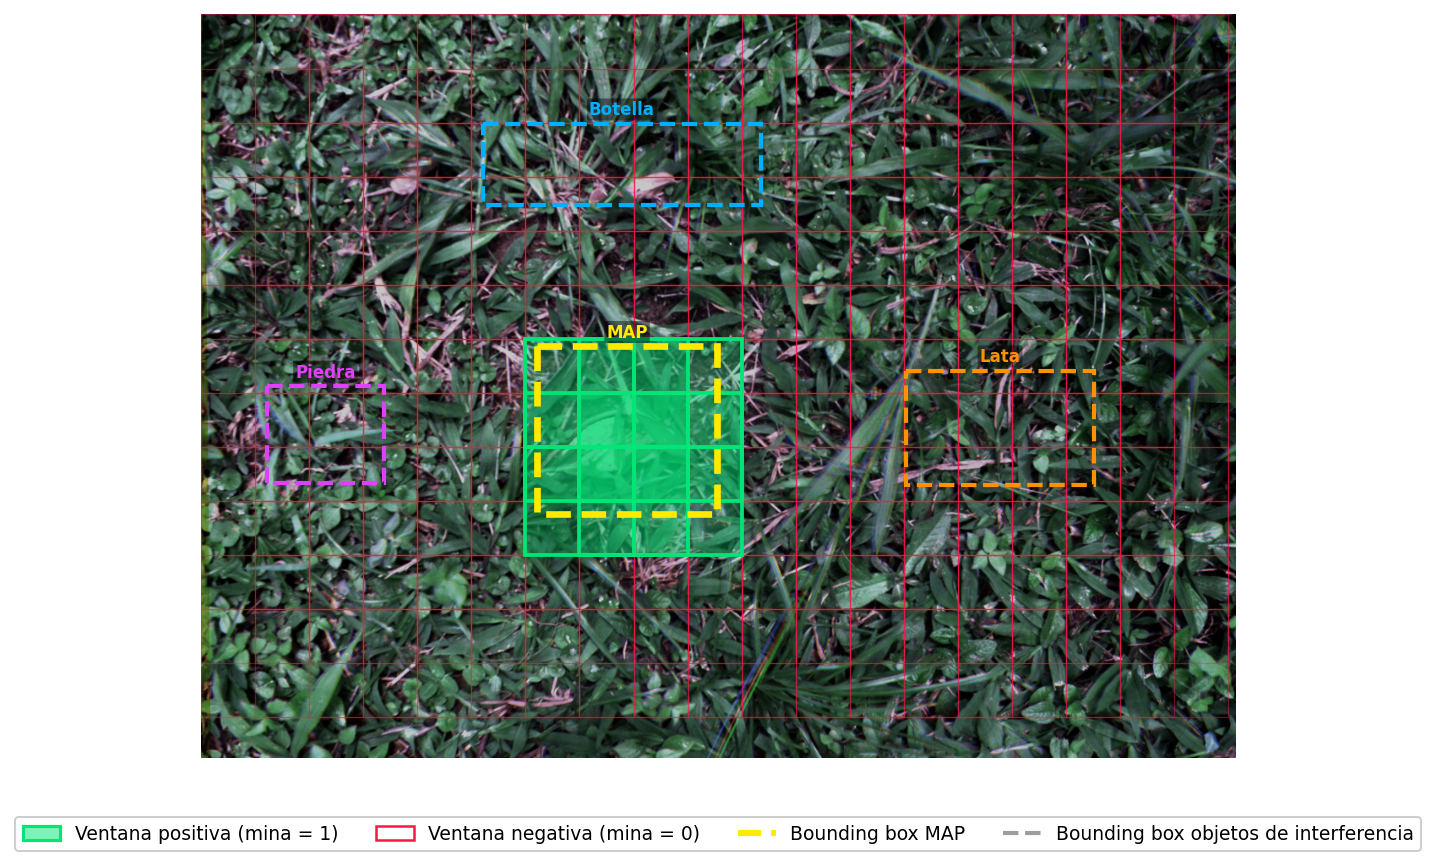
\includegraphics[width=0.7\textwidth]{figuras/comparacion_etiquetado.png}
  \caption{Etiquetado de las ventanas sobre una imagen de zona de mina (S2,
    \texttt{MINA\_7CM\_1}) y la rejilla de ventanas deslizantes
    ($128\times128$~px, paso~64). Cada cuadro representa una ventana; el color
    indica su etiqueta: positiva (verde) si su centro cae dentro del bounding
    box de la \ac{MAP} (rectángulo amarillo discontinuo), y negativa (rojo) en
    caso contrario ---incluidas las ventanas que caen sobre los objetos de
    interferencia (botella, lata y piedra, con su bounding box en color)
    (Sección~\ref{sec:segmentacion_groundtruth}).}
  \label{fig:comparacion_etiquetado}

  {\footnotesize Fuente: elaboración propia.}
\end{figure}

Es importante destacar que el reconocimiento de objetos distintos a la \ac{MAP}
no hace parte de los objetivos de este trabajo. Los objetos de interferencia se
incluyeron para analizar si su presencia puede confundir al sistema y generar
falsas alarmas, como se evalúa en la Sección~\ref{sec:analisis_fp}.

\subsection{Índices espectrales}

Para cada ventana se calculan más de 40 índices espectrales agrupados en tres
categorías: índices de vegetación (NDVI, NDRE, EVI, VARI, entre otros), índices
de suelo (BSI, CI\_soil) e índices de ratio entre bandas (NDRB, Red/Blue,
NIR/Red, y otros). Las ecuaciones de los índices principales se presentaron en
la Sección~\ref{sec:indices_espectrales}.

\subsection{Estadísticas por ventana}

Para cada índice calculado sobre la ventana, se extraen nueve estadísticas de
primer y segundo orden: media, mediana, desviación estándar, mínimo, máximo,
percentiles 25 y 75, asimetría (\textit{skewness}) y curtosis. Con más de 40
índices y 9 estadísticas cada uno, cada ventana queda representada por un vector
de \textbf{378 características}.

% ─────────────────────────────────────────────────────────────
\section{Etapa 2b: Segmentación manual del groundtruth para el aprendizaje supervisado}
\label{sec:segmentacion_groundtruth}

\subsection{Procedimiento de anotación}

Se implementó una etapa de segmentación manual del groundtruth para cada imagen
de zona de mina: se anotó un bounding box sobre la posición exacta del
artefacto, y solo las ventanas cuyo centro cae dentro del bounding box reciben
etiqueta positiva. El etiquetado opera a nivel de ventana (no de píxel), por lo
que la diferencia entre la forma rectangular del bounding box y la sección
circular de la mina tiene un efecto limitado sobre las etiquetas asignadas.

Dado que la mina puede ocupar solo una fracción del área capturada, etiquetar la
zona completa como positiva introduciría ruido: ventanas sin señal de mina
recibirían etiqueta positiva, lo que podría suprimir la contribución de bandas
cuya señal es más sutil y localizada, como el \ac{NIR} y el Red Edge. El
etiquetado preciso por bounding box evita ese ruido.

\subsection{Protocolo de anotación}

En cada sesión de campo se capturan dos imágenes por zona de mina de forma
consecutiva; cada captura corresponde exclusivamente a la zona en cuestión,
sin que otras zonas queden dentro del campo de visión:

\begin{enumerate}
  \item \textbf{Imagen de referencia (UBI):} capturada con el émbolo de la
    jeringa completamente visible sobre la superficie del suelo, lo que
    permite identificar con precisión la posición de la mina en la imagen.
  \item \textbf{Imagen de entrenamiento:} capturada con el émbolo de la
    jeringa cubierto con vegetación natural del entorno, simulando la
    condición real de ocultamiento.
\end{enumerate}

La anotación se realizó en Roboflow usando la composición RGB (bandas 3, 2
y 1) de cada zona como PNG, \textbf{únicamente como interfaz visual} --- la
base de datos se genera del TIF calibrado de 5 bandas, no del PNG. Con la imagen
imagen de referencia, se dibujó un bounding box sobre la región de la mina (clase
\texttt{MAP}) y se exportaron las anotaciones en formato COCO JSON.

\subsection{Transferencia de anotaciones al TIF calibrado}

Las coordenadas del bounding box anotado en la imagen de referencia se
transfieren al TIF calibrado de 5 bandas. Dado que existe un pequeño
desplazamiento entre la imagen de referencia y la imagen de entrenamiento
---capturadas en instantes distintos---, se corrió el algoritmo
\ac{SIFT}+RANSAC directamente sobre la imagen de referencia para registrarla
con la imagen de entrenamiento antes de usar las coordenadas. Lo que se almacena
para el entrenamiento son las coordenadas del bounding box (centro y dimensiones,
en formato COCO JSON), no la imagen de referencia.

Una ventana recibe etiqueta \texttt{tiene\_mina=1} solo si su centro cae dentro
del bounding box; de lo contrario recibe \texttt{tiene\_mina=0}, incluso si
pertenece a una imagen de zona de mina. Con el conjunto de datos completo S2--S7
este etiquetado produjo 487 positivos y 14\,414 negativos (ratio 30:1).


% -------------------------------------------------------------
\section{Etapa 3: Clasificación}

\subsection{Clasificador de desarrollo: Random Forest}
\label{sec:clasificador_rf}

La elección de \ac{RF} se fundamenta en tres propiedades útiles en la etapa
temprana del experimento:

\begin{itemize}
  \item \textbf{Robustez con datos escasos y de alta dimensionalidad.}
    El conjunto de entrenamiento disponible en esta etapa contaba con 487
    ventanas positivas (mina) frente a 378 características, un ratio bajo
    que puede comprometer otros clasificadores. El \ac{RF} maneja bien esta
    condición porque submuestrea características en cada árbol, evitando que
    la alta dimensionalidad domine el ajuste, y no requiere escalado previo
    ni selección manual de variables.
  \item \textbf{Tolerancia al desbalance de clases.} El enfoque de ventana
    deslizante genera de forma inherente un desbalance pronunciado: dado que la
    mina ocupa solo una fracción de la imagen, la mayoría de las ventanas no
    contienen el artefacto --- en la base de datos S2--S7 se obtuvieron
    aproximadamente 30 ventanas negativas por cada positiva. El \ac{RF} tolera
    bien esta condición y, además, el desbalance se corrige de forma explícita
    mediante submuestreo 1:1 al entrenar (Sección~\ref{sec:balanceo}), estrategia
    aplicada por igual a todos los clasificadores comparados.
  \item \textbf{Importancia de características interpretable.} Es posible
    identificar qué estadísticos de índices espectrales son más discriminativos,
    aportando valor diagnóstico independiente de la métrica de exactitud.
\end{itemize}

El modelo se configuró con 100 árboles (\texttt{n\_estimators = 100}),
valor por defecto de scikit-learn que estabiliza las estimaciones de importancia
de características sin costo computacional excesivo; y \texttt{max\_depth = 10},
que limita la profundidad de cada árbol para reducir el sobreajuste con el número
reducido de muestras positivas disponibles. Una vez completada la base de datos
con seis sesiones, se realizó la comparación formal de clasificadores descrita en
la Sección~\ref{sec:comparacion_clasificadores}.



\subsection{Manejo del desbalance de clases}
\label{sec:balanceo}

El etiquetado por bounding box produce 487 ventanas positivas frente a 14\,414
negativas (ratio~30:1). Entrenar directamente sobre esa distribución sesga al
clasificador hacia la clase mayoritaria y degrada la sensibilidad, la métrica más
crítica en este problema. Para corregirlo se aplica \textbf{submuestreo aleatorio
1:1} dentro de cada pliegue de validación: en el conjunto de entrenamiento se
conservan todas las ventanas positivas y se selecciona aleatoriamente un número
igual de ventanas negativas. El submuestreo se realiza \textit{únicamente sobre el
conjunto de entrenamiento de cada pliegue}; la sesión de prueba conserva su
distribución real (30:1), de modo que las métricas se reportan sobre datos no
alterados.

El submuestreo 1:1 descarta una fracción grande de las ventanas negativas
disponibles. Para aprovecharlas sin reintroducir el desbalance, se evalúa
además la estrategia \textbf{EasyEnsemble}: se entrenan diez sub-clasificadores
XGBoost, cada uno con las 487 ventanas positivas y un subconjunto aleatorio distinto
de 487 negativas, y se promedian sus probabilidades. Así cada ventana negativa tiene
oportunidad de participar en el entrenamiento y se reduce la varianza asociada a un
único submuestreo. Esta estrategia ---aplicada por igual durante la comparación de
clasificadores (Sección~\ref{sec:comparacion_clasificadores})--- busca que la
sensibilidad y la especificidad a umbral~0.5 sean representativas, sin requerir
ajuste del umbral.

\subsection{Estrategia de validación LOSO}
\label{sec:loso}

La validación \ac{LOSO}, descrita en la Sección~\ref{sec:loso_teoria}, reserva
en cada iteración $i$ una sesión $i$ completa como prueba y entrena con las
$N-1$ restantes. Las métricas que se empleen durante la búsqueda (AUC, Sensibilidad, Especificidad)
corresponderán al promedio aritmético de los $N$ pliegues.
La Figura~\ref{fig:loso_esquema} ilustra el esquema con los seis pliegues
y garantiza que ninguna ventana de la sesión de prueba aparece durante el entrenamiento.

\begin{figure}[H]
  \centering
  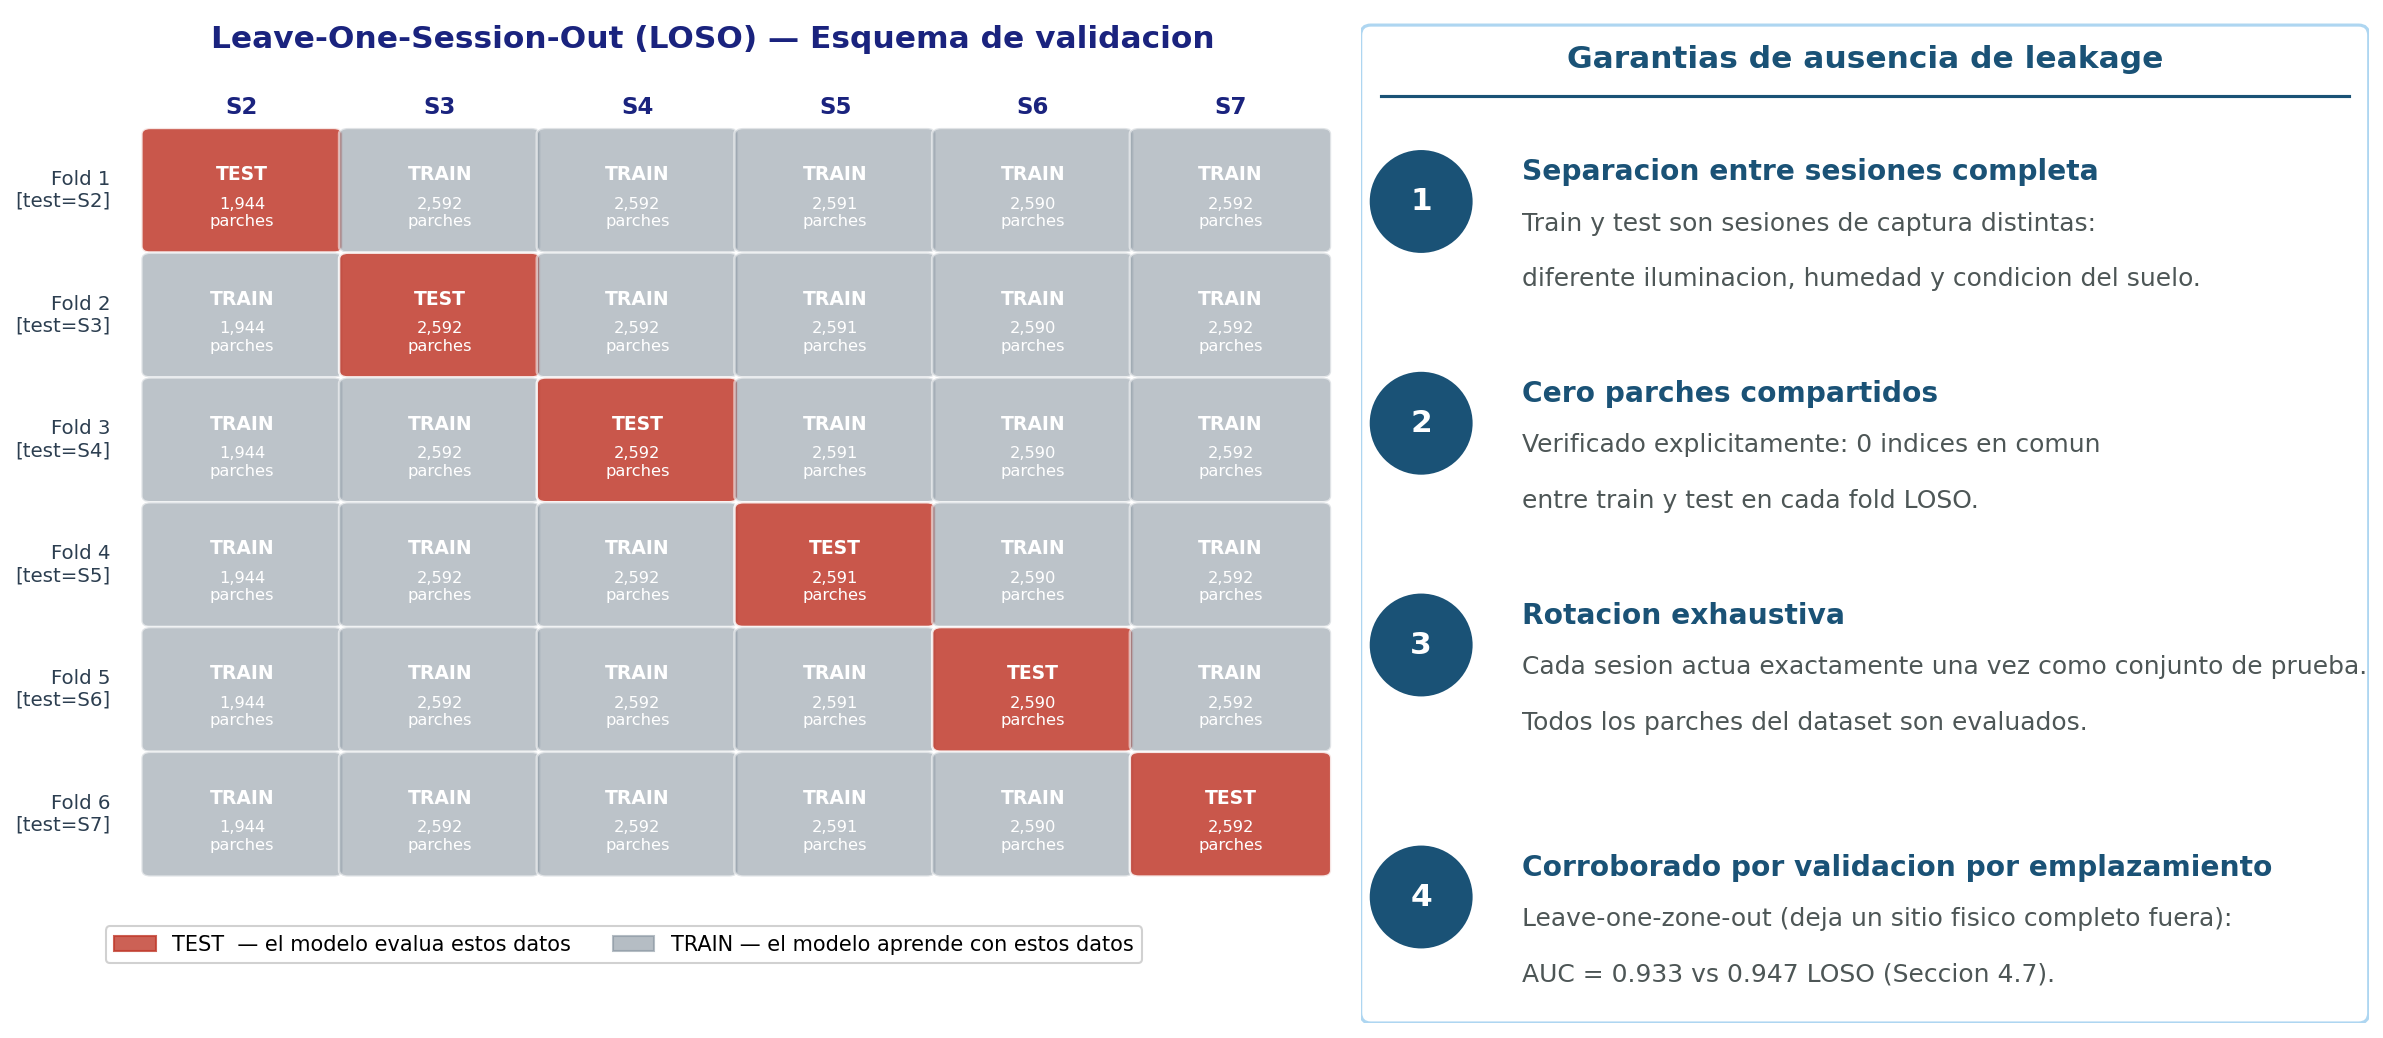
\includegraphics[width=\textwidth]{figuras/loso_justificacion.png}
  \caption{Esquema \ac{LOSO} para seis sesiones (S2--S7): cada fila
    representa un pliegue en que la sesión resaltada en rojo actúa como
    conjunto de prueba y las demás como entrenamiento. El panel derecho
    enumera las garantías de ausencia de fuga de datos, corroboradas por la
    validación por emplazamiento (\textit{leave-one-zone-out}, Sección~\ref{sec:lozo}).}
  \label{fig:loso_esquema}

  {\footnotesize Fuente: elaboración propia.}
\end{figure}

\subsection{Métricas de evaluación}

Se emplean cuatro métricas. El \textbf{AUC} (área bajo la curva \ac{ROC},
independiente del umbral; 0.5 equivale a clasificación aleatoria y 1.0 a
clasificación perfecta) es la métrica principal, pues mide la capacidad
discriminativa sin depender de un umbral y permite comparar configuraciones en
igualdad de condiciones. A umbral fijo~(0.5) se reportan tres métricas operativas:
\textbf{Sensibilidad} (fracción de minas detectadas --- privilegiada por la
asimetría de costos: una mina no detectada es mucho más costosa que una falsa
alarma), \textbf{Especificidad} (fracción de ventanas sin \ac{MAP} correctamente
clasificadas como negativas) y \textbf{falsos positivos por mina} (número de
falsas alarmas por cada mina realmente detectada, indicador del costo operativo de
una eventual inspección). El submuestreo 1:1 descrito en la
Sección~\ref{sec:balanceo} permite que estas tres métricas a umbral~0.5 sean
representativas.


% -------------------------------------------------------------

% ============================================================
%  CAPÍTULO 4 — RESULTADOS Y DISCUSIÓN  (reescritura thesisV2, sin Enfoque A)
% ============================================================
\chapter{Resultados y Discusión}
\label{cap:resultados}

Este capítulo presenta los resultados sobre la base de datos oficial: las
sesiones S2--S7 (6 sesiones, 14\,901 ventanas de $128\times128$~px), con
\textbf{487 ventanas positivas} (centro dentro del bounding box de la \ac{MAP})
y \textbf{14\,414 negativas}, un desbalance real de \textbf{30:1}. Todas las
métricas se obtienen con validación \ac{LOSO} (\emph{dejar una sesión fuera}).
Para corregir ese desbalance 30:1, el conjunto de entrenamiento se balancea con
\textbf{submuestreo aleatorio~1:1} dentro de cada pliegue, conservando la sesión
de prueba con su distribución real.

El hilo del capítulo es: (1)~caracterizar la firma espectral de cada clase;
(2)~validar que el cálculo de índices a nivel de imagen equivale al de ventana;
(3)~identificar qué características son discriminativas; (4)~elegir el
clasificador; (5)~reducir el número de características; (6)~reportar el modelo
final; y (7)~analizar su comportamiento por sesión, profundidad y falsos
positivos.

% -------------------------------------------------------------
\section{Firmas espectrales por clase}
\label{sec:firmas}

\textbf{Objetivo.} Analizar visualmente la capacidad discriminativa de las bandas
espectrales que captura la cámara y de los índices derivados de ellas, para verificar
---\emph{antes de entrenar ningún clasificador}--- si la \ac{MAP} se distingue de los
objetos de interferencia (botella, lata, piedra) y del control.

\textbf{Metodología.} Cada ventana se asigna a una clase según dónde cae su
centro (bounding box de Roboflow para \ac{MAP}, botella, lata y piedra; zona de
control para Control). Para cada clase se observa la \emph{distribución} de la
reflectancia por banda y de los índices, mediante diagramas de violín que
permiten comparar las clases entre sí y evaluar su separabilidad visual.

\begin{figure}[H]
  \centering
  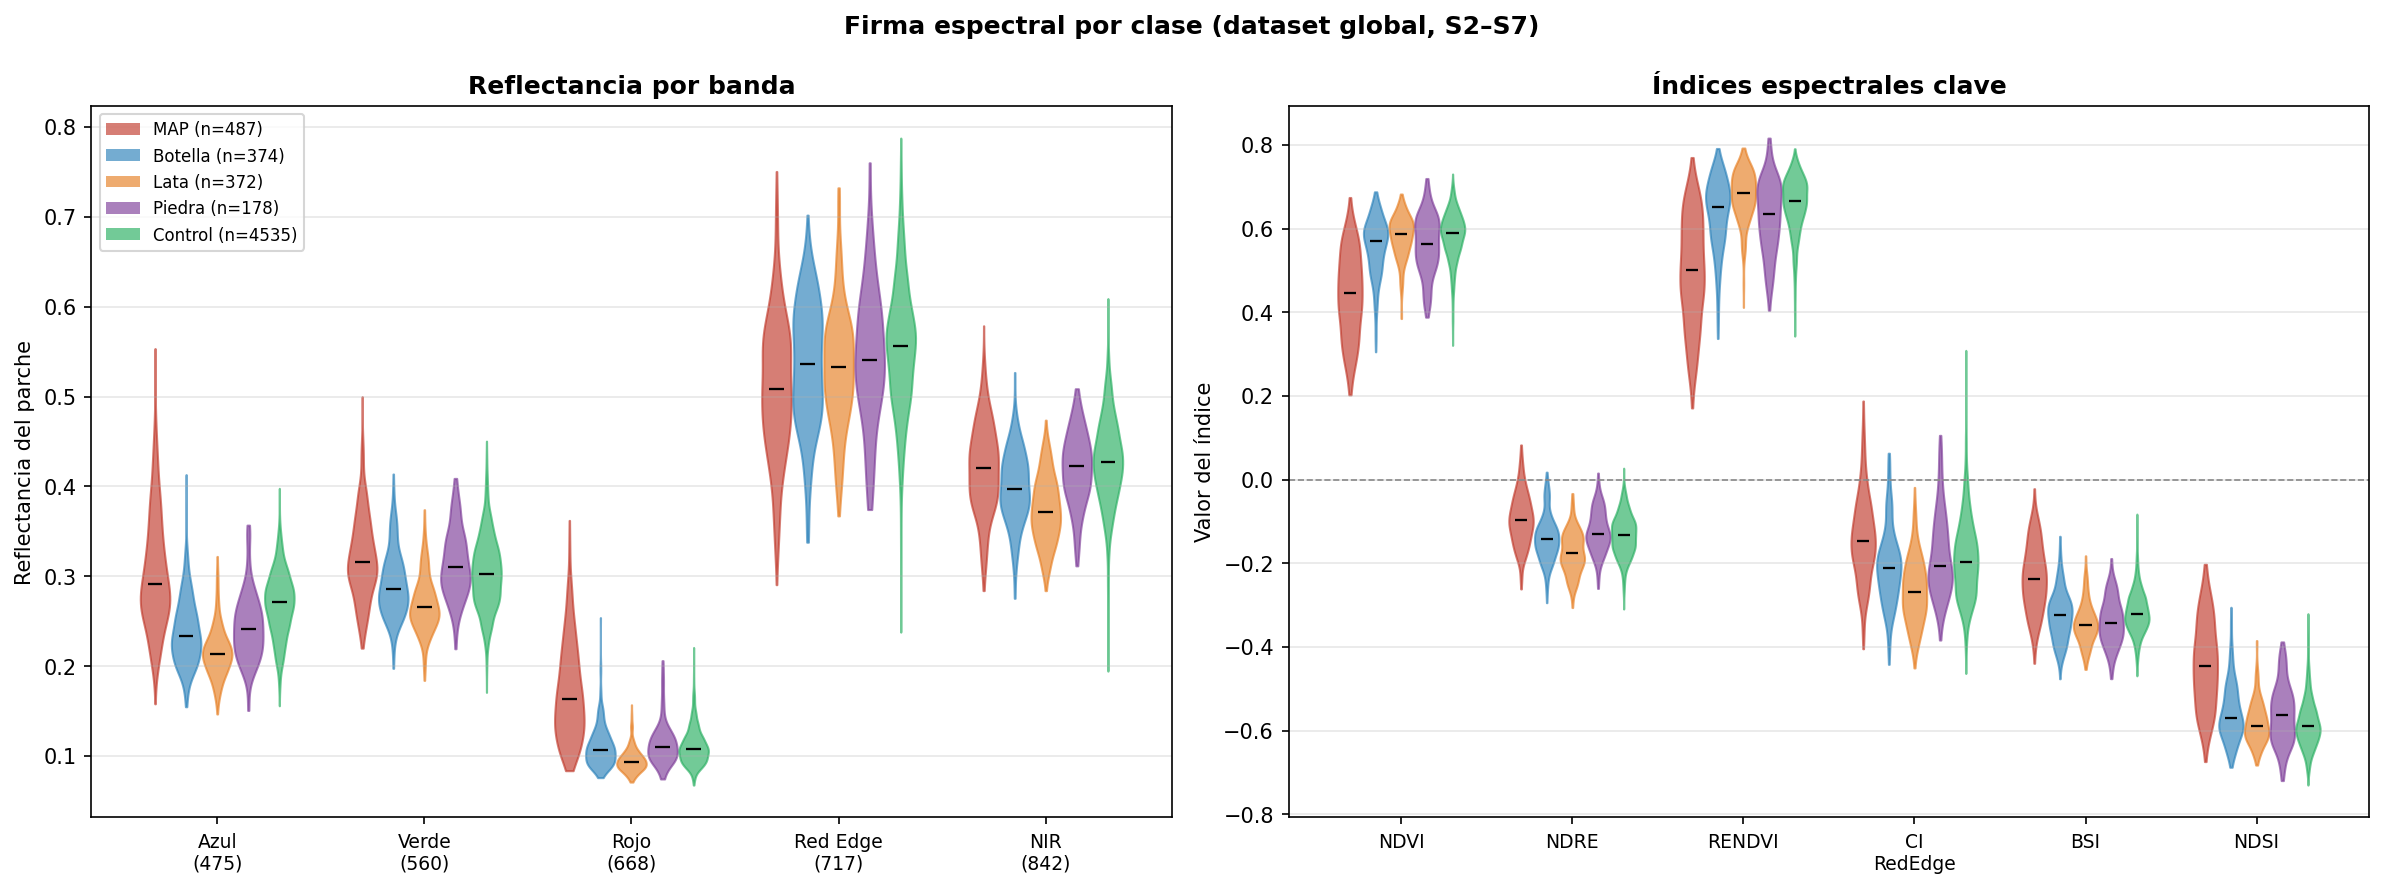
\includegraphics[width=\textwidth]{figuras/p1_violin_firma.png}
  \caption{Distribución de la firma espectral por clase (S2--S7).
    \textit{Izquierda:} reflectancia por banda. \textit{Derecha:} índices
    espectrales clave. Conteos: \ac{MAP}~=~487, Botella~=~374, Lata~=~372,
    Piedra~=~178, Control~=~4\,535.}
  \label{fig:firmas}
  \label{fig:firmas_espectrales}

  {\footnotesize Fuente: elaboración propia.}
\end{figure}

\textbf{Resultados y análisis.} En la Figura~\ref{fig:firmas}, cada violín es la
\emph{distribución} de una clase: su ancho indica dónde se concentran las ventanas
(más ancho, valores más frecuentes) y la línea negra marca la mediana; lo relevante
es comparar la altura del violín de la \ac{MAP} (rojo) con la de las demás clases.
Bajo ese criterio, en el panel de reflectancia la \ac{MAP} es la clase de
\emph{mayor} reflectancia, de forma marcada en el \textbf{Rojo} (mediana
$0.157$ frente a $\sim$$0.10$ en las demás), coherente con el suelo desnudo del
área perturbada por el enterramiento; en Azul y Verde la diferencia respecto a
Control es pequeña, así que la discriminación visible se concentra en el Rojo.
En los índices, el \textbf{NDVI} es el que más separa a la \ac{MAP} (valores
bajos por la menor cobertura vegetal activa), seguido de \textbf{NDSI} y
\textbf{RENDVI}; el NDRE y CI\_RedEdge separan menos.

No existe un índice que separe a la \ac{MAP} de forma perfecta: los violines se \emph{solapan parcialmente}. De
hecho, entre el 18\,\% y el 24\,\% de las ventanas con \ac{MAP} caen dentro del
rango intercuartil de las otras clases en NDVI. Esto anticipa que la separación
a nivel de ventana individual no será perfecta (habrá falsos positivos y
negativos) y justifica usar un clasificador que combine muchas características en
lugar de un solo índice. Los índices que aquí destacan (NDVI, NDSI, RENDVI)
reaparecerán en el análisis de importancia (Sección~\ref{sec:importancia}),
confirmando esta primera lectura.

% -------------------------------------------------------------
\section{Cálculo de índices: imagen completa vs ventana}
\label{sec:indices_global}

\textbf{Objetivo.} Evaluar si calcular los índices una sola vez sobre la imagen
completa ---y extraer después las estadísticas por ventana--- produce el mismo
resultado que recalcularlos dentro de cada ventana, y observar la diferencia en
el costo de cómputo entre ambas formas.

\textbf{Metodología.} Se extrajeron las 378 características de las dos formas
---\emph{ventana} (recalcula los índices en cada parche) y \emph{global}
(índices una vez sobre la imagen, estadísticas por ventana)--- con idéntica
semilla, y se compararon numéricamente, en métricas \ac{LOSO} (\ac{RF}, 1:1) y
en tiempo de extracción.

\textbf{Resultados.} Las características resultan \textbf{idénticas bit a bit}
($\max|\text{global}-\text{ventana}| = 0$ sobre las 378 columnas), por lo que las
métricas \ac{LOSO} coinciden exactamente (Tabla~\ref{tab:indices_modo}). El modo
global es $\sim$9\,\% más rápido en extracción.

\begin{table}[H]
\centering
\caption{Equivalencia entre el cálculo de índices por ventana y a nivel de imagen
         (\ac{RF}, 378 características, \ac{LOSO}, 1:1).}
\label{tab:indices_modo}
\small
\begin{tabular}{lccccc}
\toprule
\textbf{Modo} & \textbf{AUC} & \textbf{Sens(0.5)} & \textbf{Spec(0.5)} &
\textbf{FP/mina} & \textbf{Tiempo extracción} \\
\midrule
Ventana (por parche) & 0.915 & 0.805 & 0.856 & 5.29 & 1856 s \\
\textbf{Global (imagen)} & \textbf{0.915} & \textbf{0.805} & \textbf{0.856} &
\textbf{5.29} & \textbf{1693 s (--9\,\%)} \\
\bottomrule
\end{tabular}

  {\footnotesize Fuente: elaboración propia.}
\end{table}

\textbf{Análisis.} La equivalencia es esperable porque los índices son
operaciones \emph{píxel a píxel} (NDVI, ratios, diferencias): el valor en cada
píxel no depende de si se calcula sobre toda la imagen o sobre el parche. El
ahorro es modesto (no $\sim$4$\times$ como sugeriría el solapamiento del 50\,\%)
porque el cuello de botella son las nueve estadísticas por ventana, que se
calculan por parche en ambos modos. Se adopta el \textbf{cálculo a nivel de
imagen}: mismo resultado, algo más eficiente. El resto del capítulo usa esta
versión.

% -------------------------------------------------------------
\section{Importancia de características}
\label{sec:importancia}

\textbf{Objetivo.} Identificar las características más discriminativas
para distinguir la \ac{MAP} y determinar el papel de las bandas \ac{NIR} y Red
Edge frente al de las bandas visibles.

\textbf{Metodología.} Se promedió la importancia Gini del \ac{RF} sobre los seis
pliegues \ac{LOSO} (1:1, misma semilla). La importancia se calcula sobre las 378
características ---de bandas visibles e infrarrojas por igual---, lo que permite
comparar directamente el peso de cada dominio espectral. La
Tabla~\ref{tab:importancia} lista las 20 más importantes.

\begin{table}[H]
\centering
\caption{Top-20 características por importancia (RF, \ac{LOSO}, S2--S7).
         En negrita las que involucran \ac{NIR} (842~nm) o Red Edge (717~nm).}
\label{tab:importancia}
\small
\begin{tabular}{cll c cll}
\toprule
\# & Índice & Estad. & & \# & Índice & Estad. \\
\midrule
1  & Red & mean        & & 11 & \textbf{RedEdge} & min \\
2  & SI & std          & & 12 & Red\_Green & p75 \\
3  & GRVI & p25        & & 13 & \textbf{NDSI} & p75 \\
4  & \textbf{RENDVI} & std & & 14 & \textbf{NDVI} & p25 \\
5  & VARI & p25        & & 15 & Red & std \\
6  & \textbf{NIR\_Red} & p25 & & 16 & \textbf{MSAVI} & p25 \\
7  & \textbf{NDVI} & std & & 17 & \textbf{NDVI} & skewness \\
8  & CI\_soil & skewness & & 18 & \textbf{RedEdge\_Red} & p25 \\
9  & \textbf{NDSVI} & std & & 19 & \textbf{RENDVI} & p25 \\
10 & \textbf{NDSI} & std & & 20 & Red & p75 \\
\bottomrule
\end{tabular}

  {\footnotesize Fuente: elaboración propia.}
\end{table}

\textbf{Resultados y análisis.} La característica más importante es del visible
(Red\_mean), pero \textbf{12 de las 20} involucran \ac{NIR} o Red Edge (RENDVI,
NIR\_Red, NDVI, NDSVI, NDSI, RedEdge, MSAVI, RedEdge\_Red): ambos dominios
contribuyen y el infrarrojo no es marginal. Esto confirma que las bandas
infrarrojas son discriminativas ---coherente con la firma espectral de la
Sección~\ref{sec:firmas}, donde NDVI/NDSI/RENDVI ya destacaban. Además, domina el
estadístico \textbf{std} (desviación estándar): RENDVI\_std, NDVI\_std,
NDSVI\_std, NDSI\_std, SI\_std, Red\_std. La importancia no se concentra en pocas
características, sino que está \emph{repartida} entre muchas ---no hay un
discriminador único.

La Figura~\ref{fig:violin_top} muestra los violines de las características más
importantes, no solo sus medias.
Revela que la \ac{MAP} tiene una \textbf{desviación estándar más alta} que las
demás clases en varios índices: dentro de la ventana de una mina, la perturbación
genera un \emph{gradiente espectral localizado} (parte alterada vs.\ entorno),
y la desviación estándar captura esa heterogeneidad mejor que el valor medio.
Esta figura es el puente entre la firma promedio (Sección~\ref{sec:firmas}) y la
importancia: la \ac{MAP} no se distingue tanto por su valor medio como por su
\emph{variabilidad local}. La equivalencia global/ventana también se cumple aquí
(importancias idénticas).

\begin{figure}[H]
  \centering
  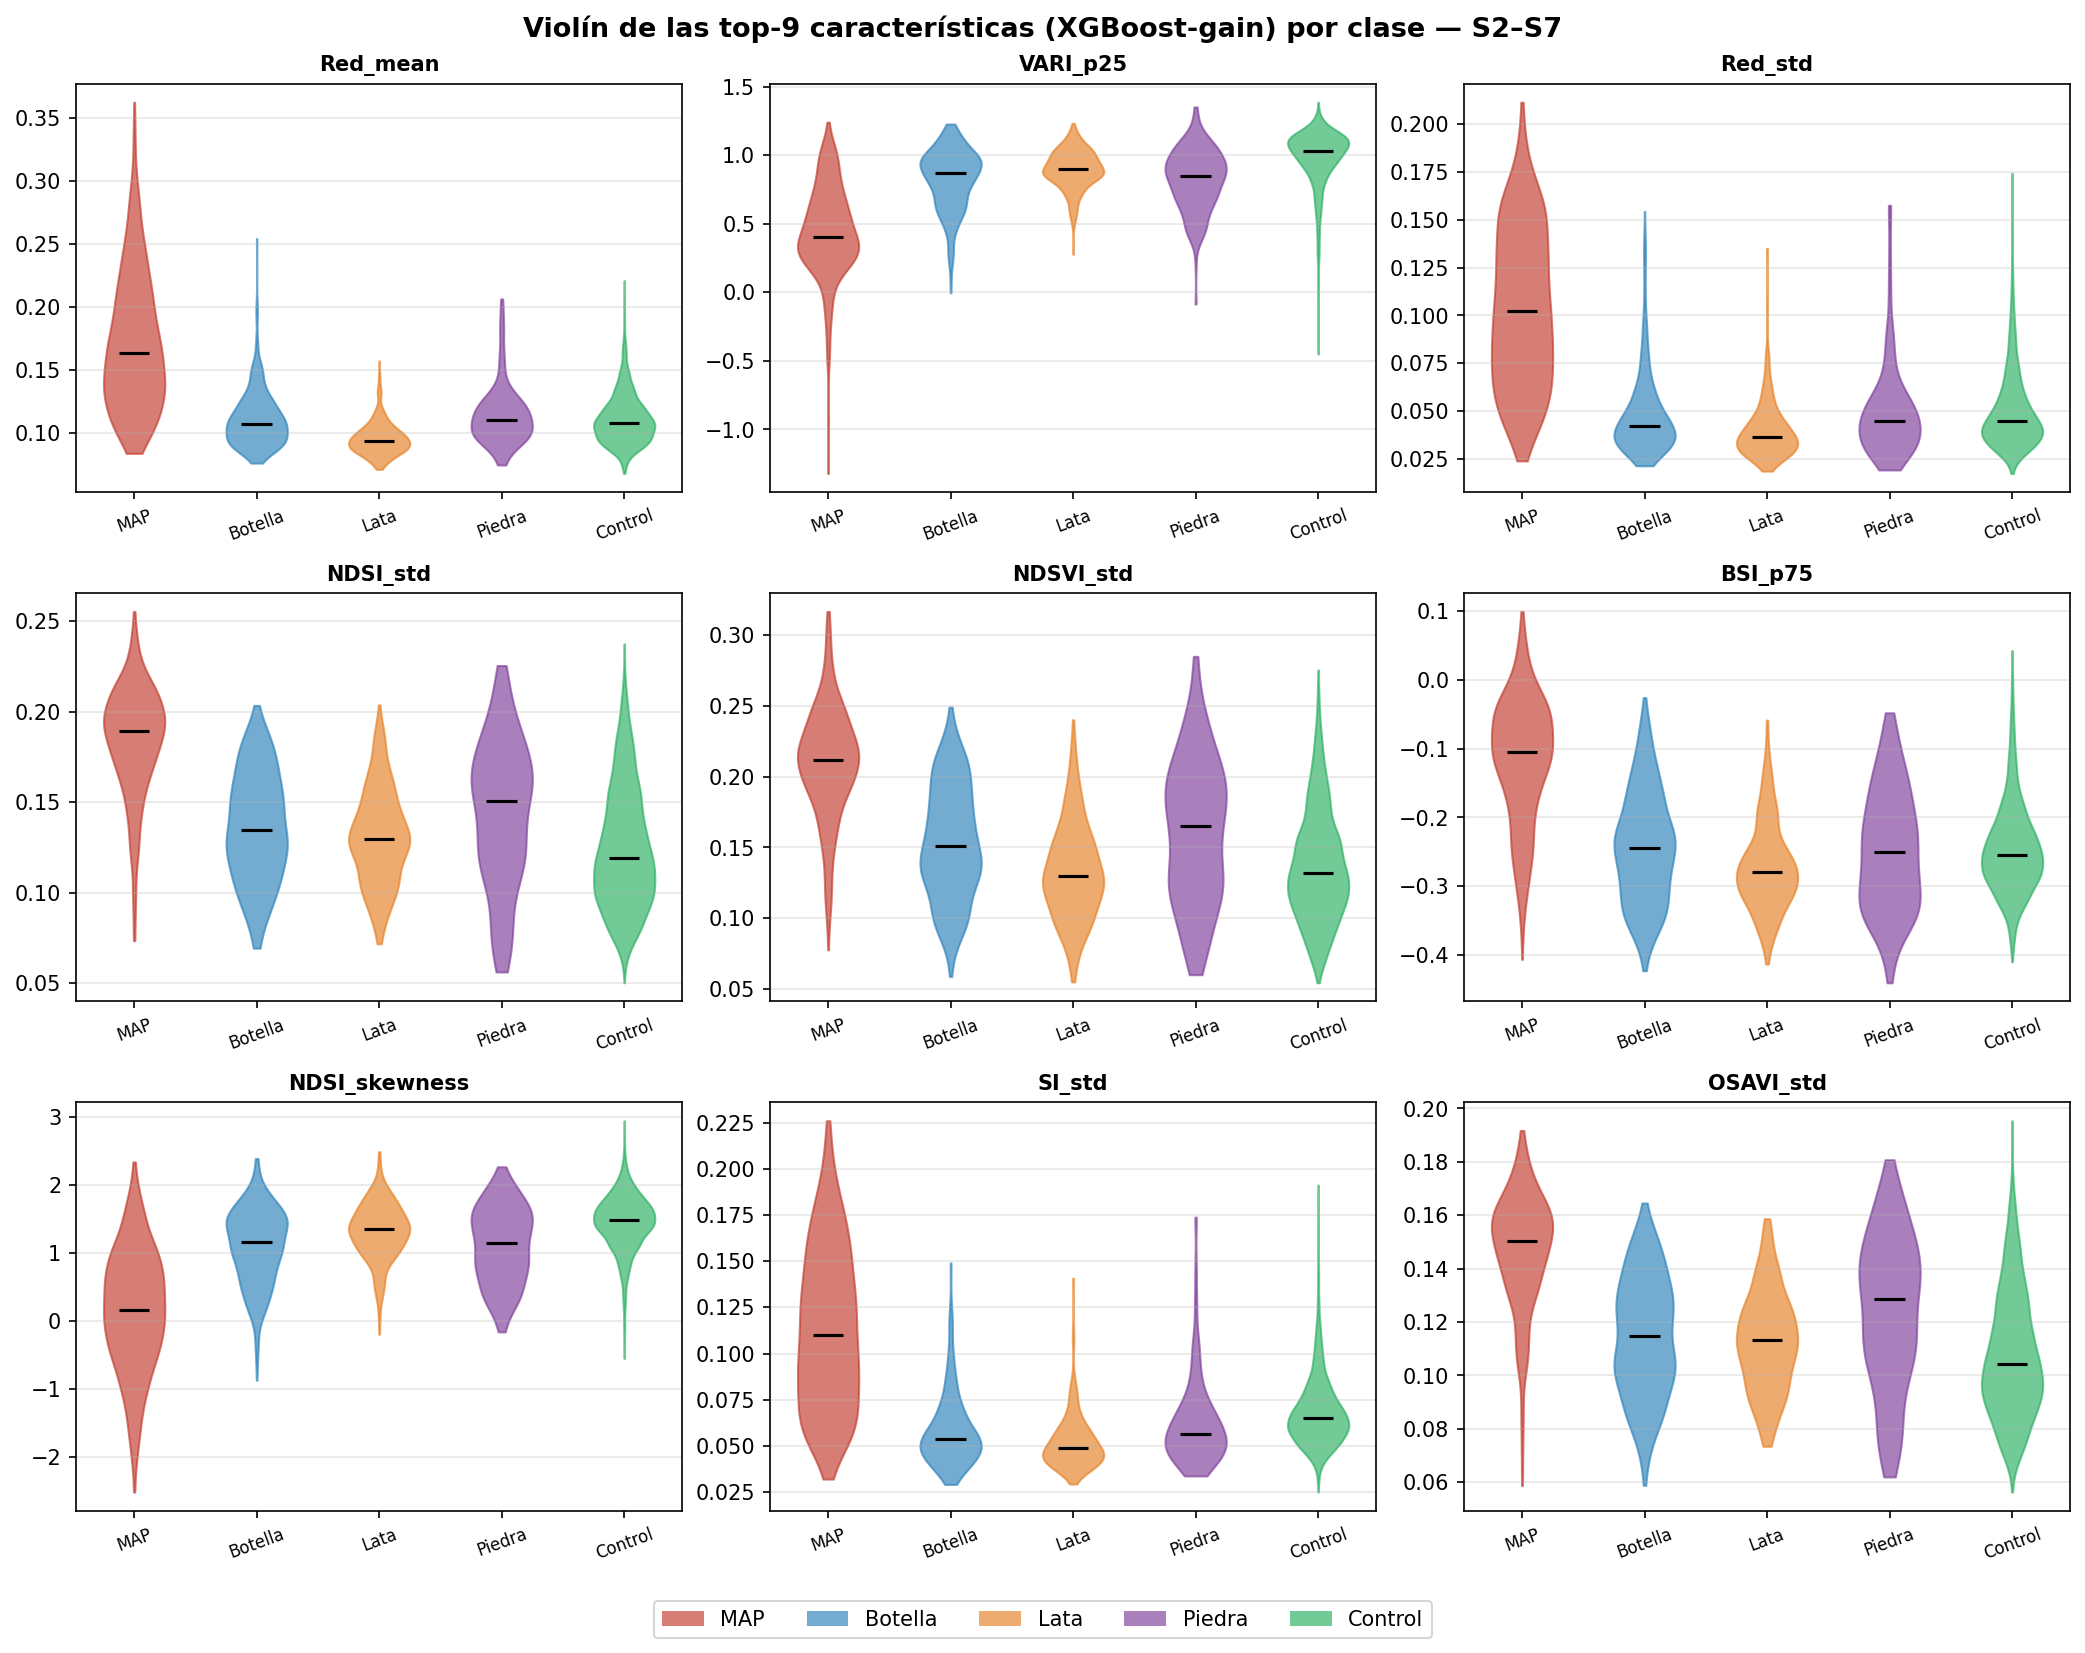
\includegraphics[width=\textwidth]{figuras/violin_top_features.png}
  \caption{Violín de las características más importantes por clase. La \ac{MAP}
    (rojo) presenta mayor desviación estándar (Red\_std, NDSI\_std, NDSVI\_std,
    SI\_std\ldots), señal de la heterogeneidad local que genera la perturbación.}
  \label{fig:violin_top}

  {\footnotesize Fuente: elaboración propia.}
\end{figure}

% -------------------------------------------------------------
\section{Comparación de clasificadores}
\label{sec:clasificadores}
\label{sec:comparacion_clasificadores}

\textbf{Objetivo.} Elegir el clasificador, evaluando rendimiento y costo
computacional.

\textbf{Metodología.} Se compararon \ac{RF}, \ac{SVM} (kernel RBF), XGBoost y
\textbf{EasyEnsemble~x10} (diez XGBoost, cada uno con un submuestreo 1:1 distinto,
probabilidades promediadas), con las 378 características y \ac{LOSO}. Los
hiperparámetros se fijaron para todos los clasificadores, garantizando una
comparación homogénea: \ac{RF} con 100 árboles y profundidad máxima~10; \ac{SVM}
con $C=1$, $\gamma=$\,\texttt{scale} y \texttt{StandardScaler} ajustado por
pliegue; XGBoost ---y cada clasificador base de EasyEnsemble--- con 200 árboles,
profundidad máxima~4, tasa de aprendizaje~0.1 y submuestreo de filas y columnas
de~0.8. Para cada clasificador se midió, además de las métricas de detección, el
tiempo de entrenamiento e inferencia como medida del costo computacional.

\begin{table}[H]
\centering
\caption{Comparación de clasificadores (378 características, \ac{LOSO}, 1:1).}
\label{tab:clasificadores}
\small
\begin{tabular}{lccccc}
\toprule
\textbf{Clasificador} & \textbf{AUC} & \textbf{Sens(0.5)} & \textbf{Spec(0.5)} &
\textbf{FP/mina} & \textbf{Inferencia} \\
\midrule
Random Forest & 0.915 $\pm$ 0.023 & 0.805 & 0.856 & 5.29 & 22.9 µs/vent. \\
SVM (RBF) & 0.929 $\pm$ 0.010 & 0.758 & 0.880 & 4.70 & 108 µs/vent. \\
XGBoost & 0.941 $\pm$ 0.014 & 0.817 & 0.885 & 4.15 & \textbf{2.6 µs/vent.} \\
\textbf{EasyEnsemble x10} & \textbf{0.945 $\pm$ 0.013} & \textbf{0.832} &
0.883 & 4.16 & 29.7 µs/vent. \\
\bottomrule
\end{tabular}

  {\footnotesize Fuente: elaboración propia.}
\end{table}

\textbf{Resultados.} Como resume la Tabla~\ref{tab:clasificadores}, \textbf{EasyEnsemble} es el mejor en \ac{AUC} (0.945) y
sensibilidad (0.832), y el más estable. La Figura~\ref{fig:matrices} presenta una matriz de
confusión por clasificador: las filas son la clase real y las columnas la
predicción del modelo, de modo que el porcentaje de cada fila indica qué fracción
de esa clase se clasificó bien (no-minas correctas en la fila superior, minas
detectadas en la inferior). EasyEnsemble domina las dos filas a la vez: detecta
más minas \emph{y} produce menos falsas alarmas (1\,684 FP, el menor).

\begin{figure}[H]
  \centering
  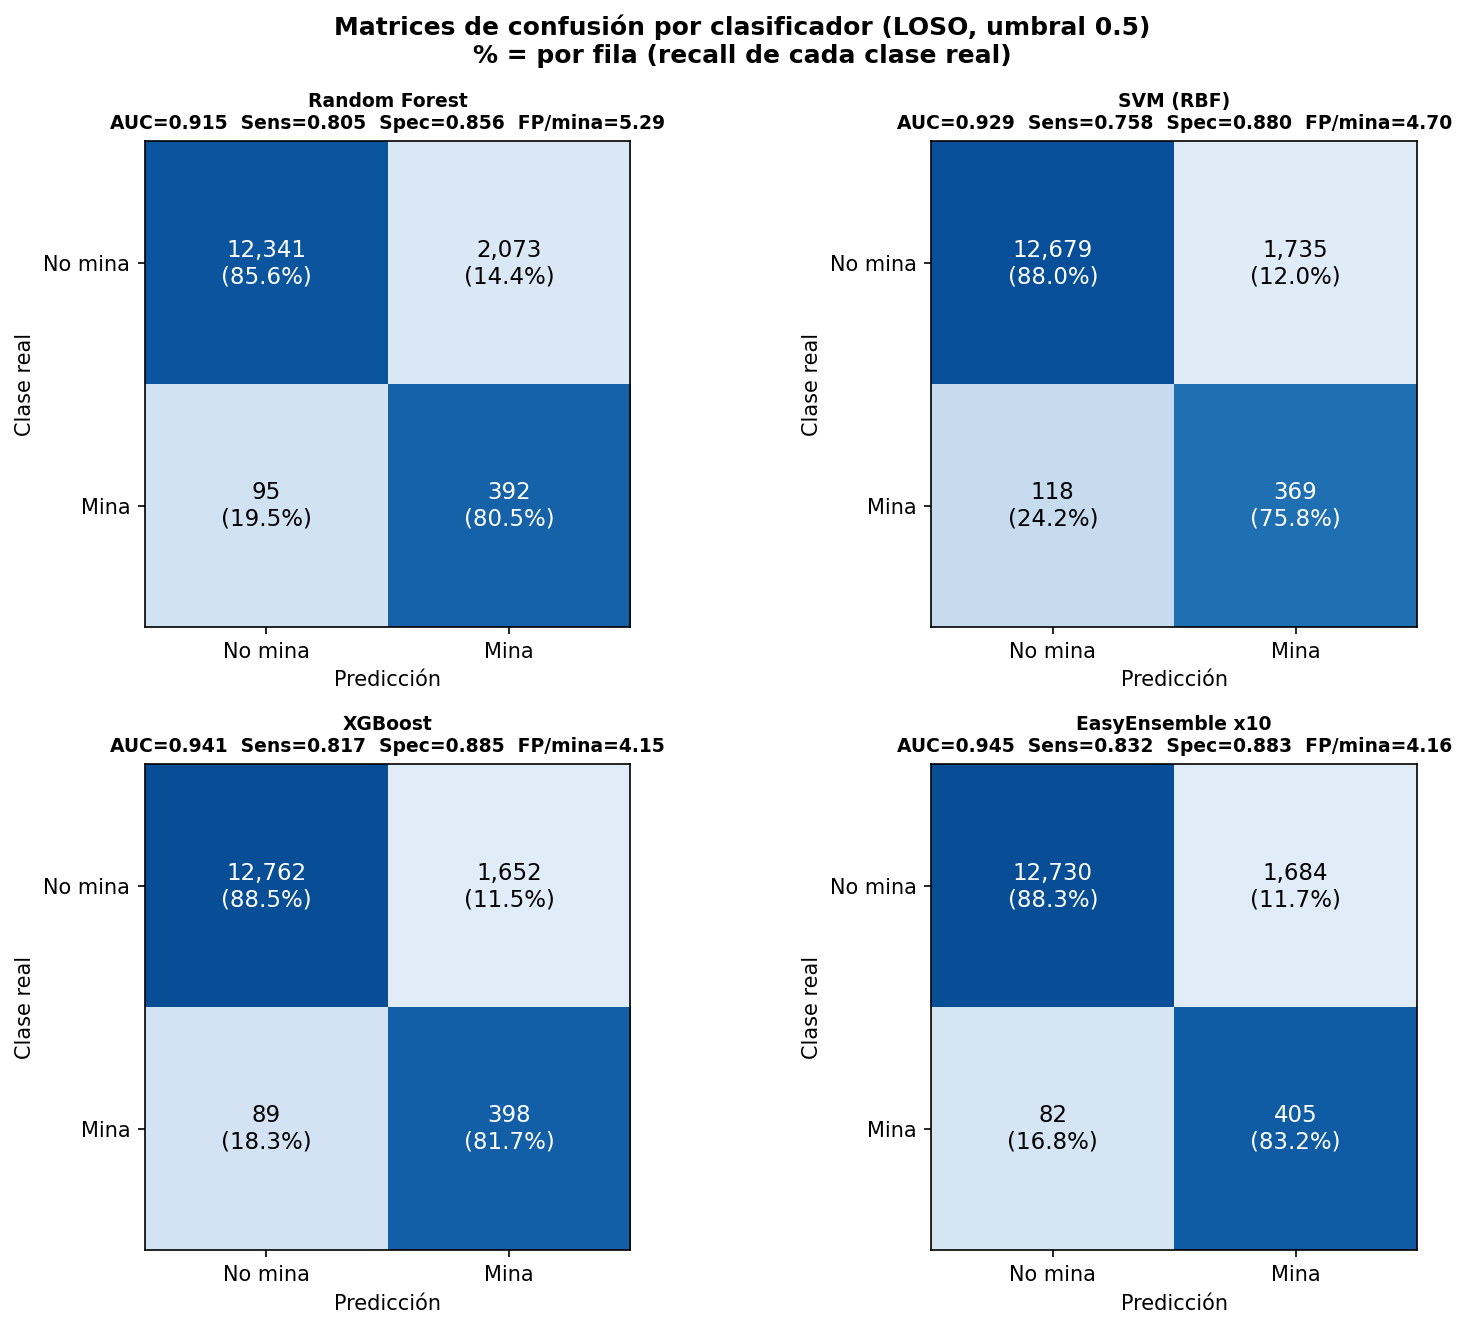
\includegraphics[width=\textwidth]{figuras/p3c_matrices.png}
  \caption{Matrices de confusión por clasificador (\ac{LOSO}, umbral~0.5;
    \% por fila = recall de cada clase). EasyEnsemble equilibra mejor ambas filas.}
  \label{fig:matrices}

  {\footnotesize Fuente: elaboración propia.}
\end{figure}

\textbf{Análisis de complejidad.} EasyEnsemble cuesta $\sim$10$\times$ más en
entrenamiento e inferencia que un solo XGBoost (son diez modelos), por una
ganancia pequeña ($+0.004$ \ac{AUC}). Sin embargo, en términos absolutos la
inferencia es trivial: $\sim$6~ms por imagen frente a $\sim$25~s de extracción.
El sobrecosto es despreciable para análisis post-captura, así que se elige
\textbf{EasyEnsemble} por sus mejores métricas; XGBoost queda como alternativa
ligera (11$\times$ más rápido, $-0.004$ \ac{AUC}) para hardware limitado.

% -------------------------------------------------------------
\section{Selección de características}
\label{sec:seleccion_k}

\textbf{Objetivo.} Definir cómo se seleccionan las características del modelo
final: con qué medida de importancia se ordenan y cuántas conservar sin perder
rendimiento.

\textbf{Metodología.} Las características se ordenan por la \textbf{importancia de
ganancia de XGBoost}, calculada dentro de cada pliegue \ac{LOSO} (consistente con
el clasificador final, sin fuga de información); para justificar esa elección se
compara contra ordenarlas por la importancia Gini de \ac{RF}. Luego se barre el
número de características $k$ con \textbf{paso uniforme de 10}
($k=10,20,\ldots,378$) y se elige, con un criterio explícito, el menor $k$ que
alcanza el 99.5\,\% del \ac{AUC} máximo (la meseta de rendimiento).

\textbf{Método de selección.} Ordenar por la ganancia de XGBoost iguala o supera a
ordenar por la importancia de \ac{RF} (Figura~\ref{fig:metodo_sel}): a $k=50$,
\ac{AUC}~0.942 frente a 0.935; a $k=100$, 0.947 frente a 0.940. Como el
clasificador final es XGBoost, ordenar con su \emph{propia} medida de importancia
es lo consistente y, además, no penaliza el rendimiento.

\begin{figure}[H]
  \centering
  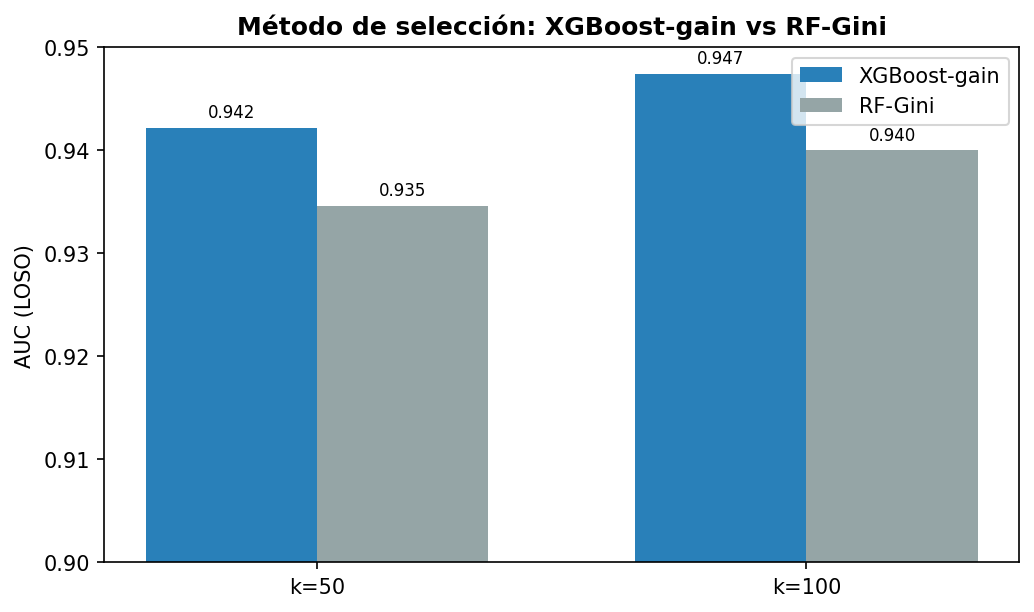
\includegraphics[width=0.62\textwidth]{figuras/p4_metodo_seleccion.png}
  \caption{Método de selección: ordenar las características por la ganancia de
    XGBoost vs.\ por la importancia Gini de \ac{RF} (\ac{AUC} \ac{LOSO}, $k=50$
    y $k=100$).}
  \label{fig:metodo_sel}

  {\footnotesize Fuente: elaboración propia.}
\end{figure}

\textbf{Número de características.} La Figura~\ref{fig:barrido_k} traza el \ac{AUC}
(y la sensibilidad y especificidad) frente a $k$: la curva sube rápido y luego se
aplana formando una meseta. Bajo el criterio anterior, el menor $k$ admisible es
$k=60$. Se elige \textbf{$k=70$} por ser el punto de la meseta que \emph{domina} a
$k=60$ en todas las métricas (AUC 0.947, Sens 0.823, Spec 0.884, FP/mina 4.16
vs.\ 0.944/0.819/0.882/4.26), priorizando la sensibilidad ---la métrica crítica en
detección de minas--- por solo diez características más. El criterio alternativo de
\emph{importancia acumulada} se descarta: como la importancia está repartida entre
muchas características, exigir el 90\,\% acumulado llevaría a $k=235$ ---casi
todas--- para el mismo \ac{AUC}.

\begin{figure}[H]
  \centering
  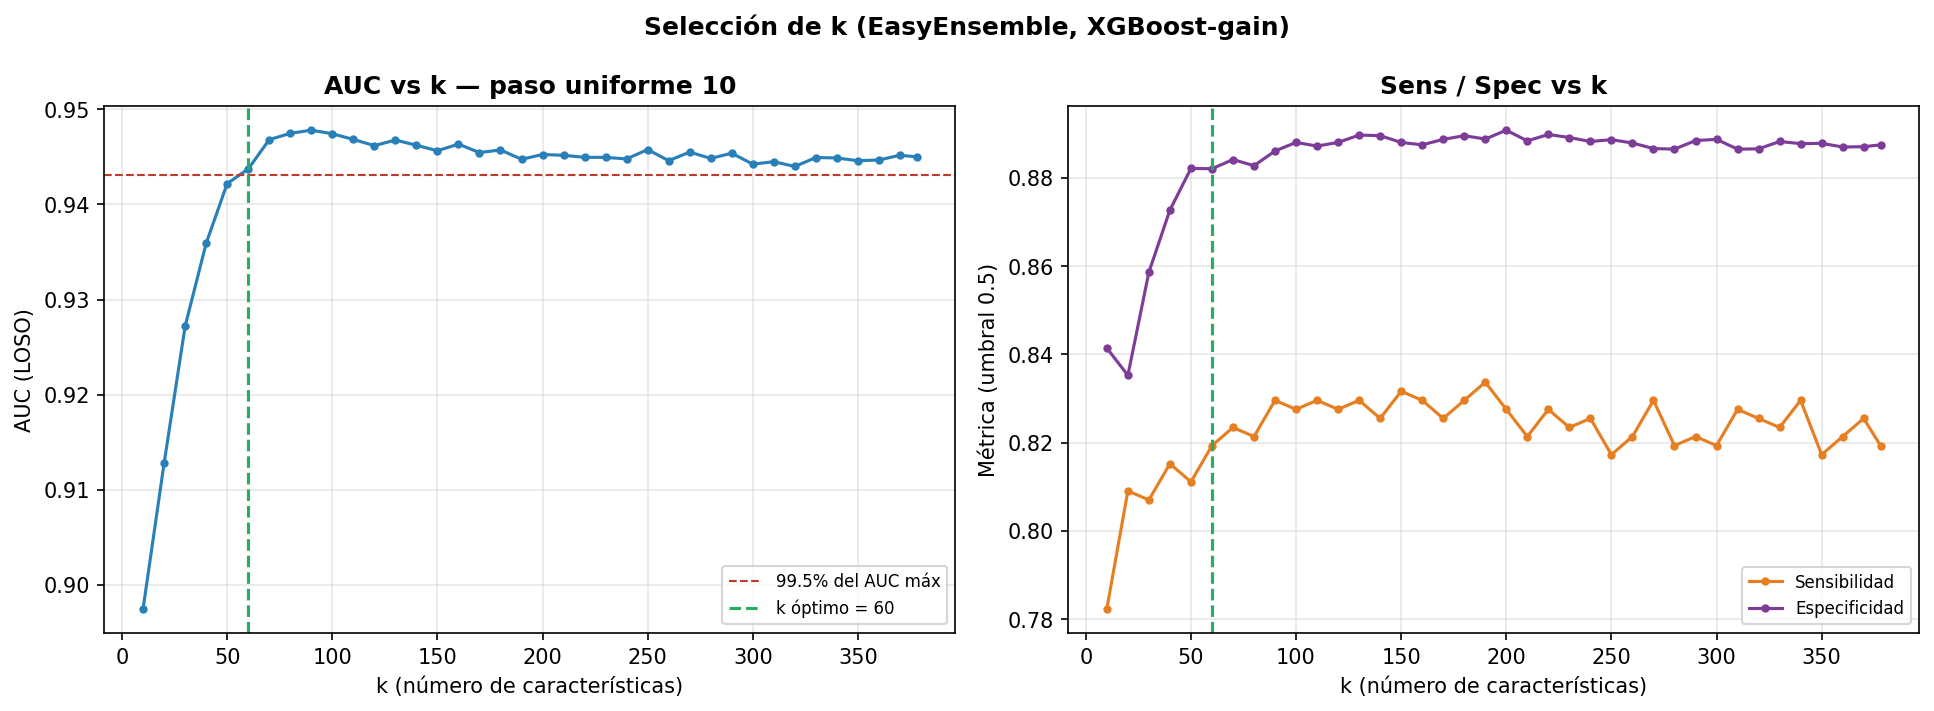
\includegraphics[width=\textwidth]{figuras/p4_barrido_k.png}
  \caption{Selección de $k$ (EasyEnsemble, XGBoost-gain). \textit{Izquierda:}
    \ac{AUC} vs.\ $k$ con el criterio del 99.5\,\%. \textit{Derecha:}
    sensibilidad y especificidad vs.\ $k$.}
  \label{fig:barrido_k}

  {\footnotesize Fuente: elaboración propia.}
\end{figure}

% -------------------------------------------------------------
\section{Modelo final: métricas con LOSO por fold}
\label{sec:modelo_final}

\textbf{Objetivo.} Reportar el rendimiento del modelo final ---EasyEnsemble~x10,
top-70 características--- bajo \ac{LOSO}.

\textbf{Metodología.} Se aplica el modelo final ---EasyEnsemble~x10 con las
top-70 características seleccionadas por ganancia de XGBoost dentro de cada
pliegue--- bajo \ac{LOSO}, y se reportan las métricas por sesión a umbral~0.5.

\begin{table}[H]
\centering
\caption{Métricas \ac{LOSO} por fold del modelo final (EasyEnsemble~x10,
         top-70, umbral~0.5).}
\label{tab:modelo_final}
\small
\begin{tabular}{lccccccc}
\toprule
\textbf{Fold} & \textbf{AUC} & \textbf{Sens} & \textbf{Spec} &
\textbf{TP} & \textbf{FN} & \textbf{FP} & \textbf{TN} \\
\midrule
S2 & 0.936 & 0.827 & 0.898 & 62 & 13 & 191 & 1\,678 \\
S3 & 0.946 & 0.964 & 0.669 & 81 & 3  & 831 & 1\,677 \\
S4 & 0.942 & 0.770 & 0.921 & 67 & 20 & 198 & 2\,307 \\
S5 & 0.950 & 0.815 & 0.916 & 66 & 15 & 212 & 2\,298 \\
S6 & 0.958 & 0.872 & 0.938 & 68 & 10 & 156 & 2\,356 \\
S7 & 0.948 & 0.695 & 0.967 & 57 & 25 & 82  & 2\,428 \\
\midrule
\textbf{Prom.} & \textbf{0.947} & \textbf{0.823} & \textbf{0.884} &
401 & 86 & 1\,670 & 12\,744 \\
\bottomrule
\end{tabular}

  {\footnotesize Fuente: elaboración propia.}
\end{table}

\textbf{Resultados.} El modelo final alcanza \textbf{AUC~=~0.947, sensibilidad
82.3\,\%, especificidad 88.4\,\% y $\sim$4.2 falsos positivos por mina}. En la
matriz de confusión (Figura~\ref{fig:confusion_final}), de las 487 minas reales
el sistema detecta 401 y se le escapan 86; de las 14\,414 ventanas sin mina,
12\,744 se rechazan correctamente y 1\,670 producen falsas alarmas. El porcentaje
de cada fila es el recall de esa clase (sensibilidad en la fila de mina,
especificidad en la de no-mina).

\begin{figure}[H]
  \centering
  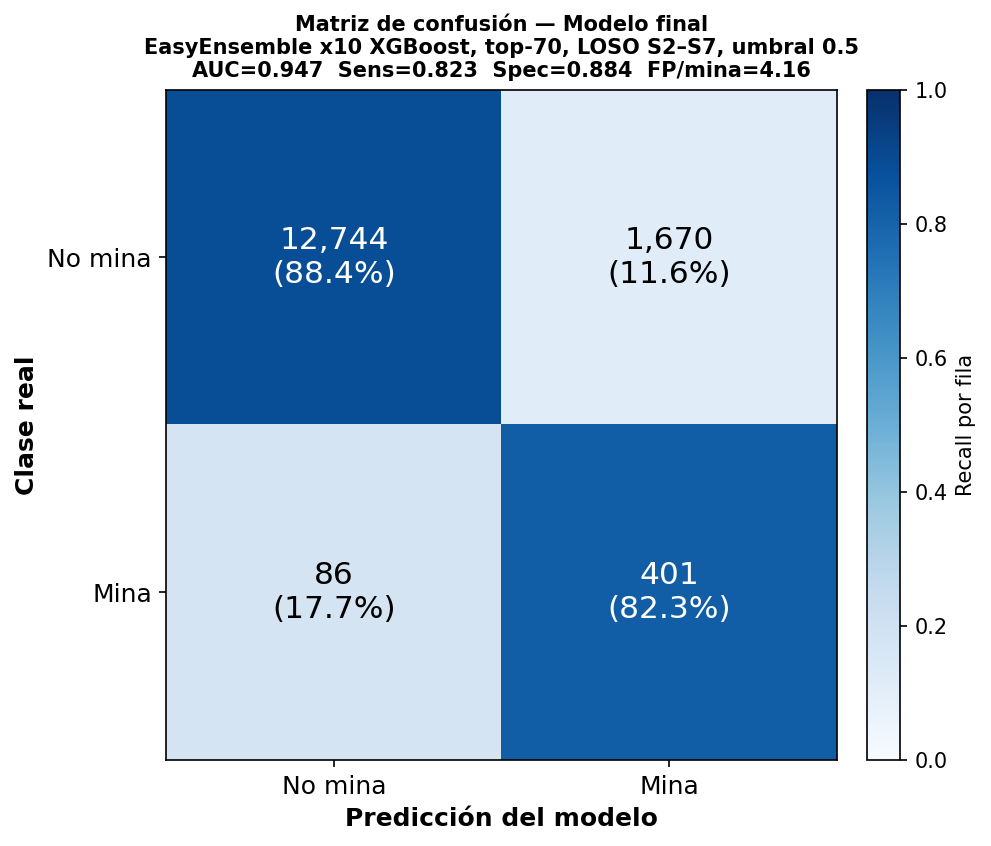
\includegraphics[width=0.62\textwidth]{figuras/p5_matriz_confusion.png}
  \caption{Matriz de confusión del modelo final (EasyEnsemble~x10, top-70,
    \ac{LOSO} S2--S7, umbral~0.5). Conteos reales; el porcentaje de cada fila es
    el recall de esa clase.}
  \label{fig:confusion_final}

  {\footnotesize Fuente: elaboración propia.}
\end{figure}

\textbf{Análisis.} El comportamiento varía entre sesiones (Tabla~\ref{tab:modelo_final}): S3
detecta casi todas las minas (Sens 0.964) pero genera muchas falsas alarmas
(Spec 0.669), mientras que S7 es lo contrario (Spec 0.967, Sens 0.695). Esta
variabilidad refleja que es un \emph{problema difícil}: las clases se solapan, no
hay un discriminador marcado y las condiciones de cada sesión afectan el balance
entre detección y falsas alarmas. Aun así, el \ac{AUC} se mantiene alto y estable
($0.947 \pm 0.007$) en las seis sesiones.

Para ilustrar el comportamiento del modelo sobre imágenes que \emph{no vio durante
el entrenamiento}, la Figura~\ref{fig:mapa} aplica el modelo final a dos imágenes de
la Sesión~2, predichas ---bajo \ac{LOSO}--- por el modelo entrenado únicamente con
las otras cinco sesiones. En la \textbf{zona de mina} (fila superior) la alta
probabilidad se concentra sobre la \ac{MAP} ---sus nueve ventanas se detectan--- y
los falsos positivos quedan en el borde difuso del suelo perturbado que la rodea
(su análisis se presenta en la Figura~\ref{fig:fp_espacial}, Sección~\ref{sec:fp_objetos}). En la \textbf{zona de
control} (fila inferior, sin mina enterrada) el modelo permanece prácticamente
apagado: solo 2 de 216 ventanas superan el umbral. El sistema enciende donde hay
mina y se mantiene silencioso donde no la hay, sobre imágenes nunca vistas en
entrenamiento.

\begin{figure}[H]
  \centering
  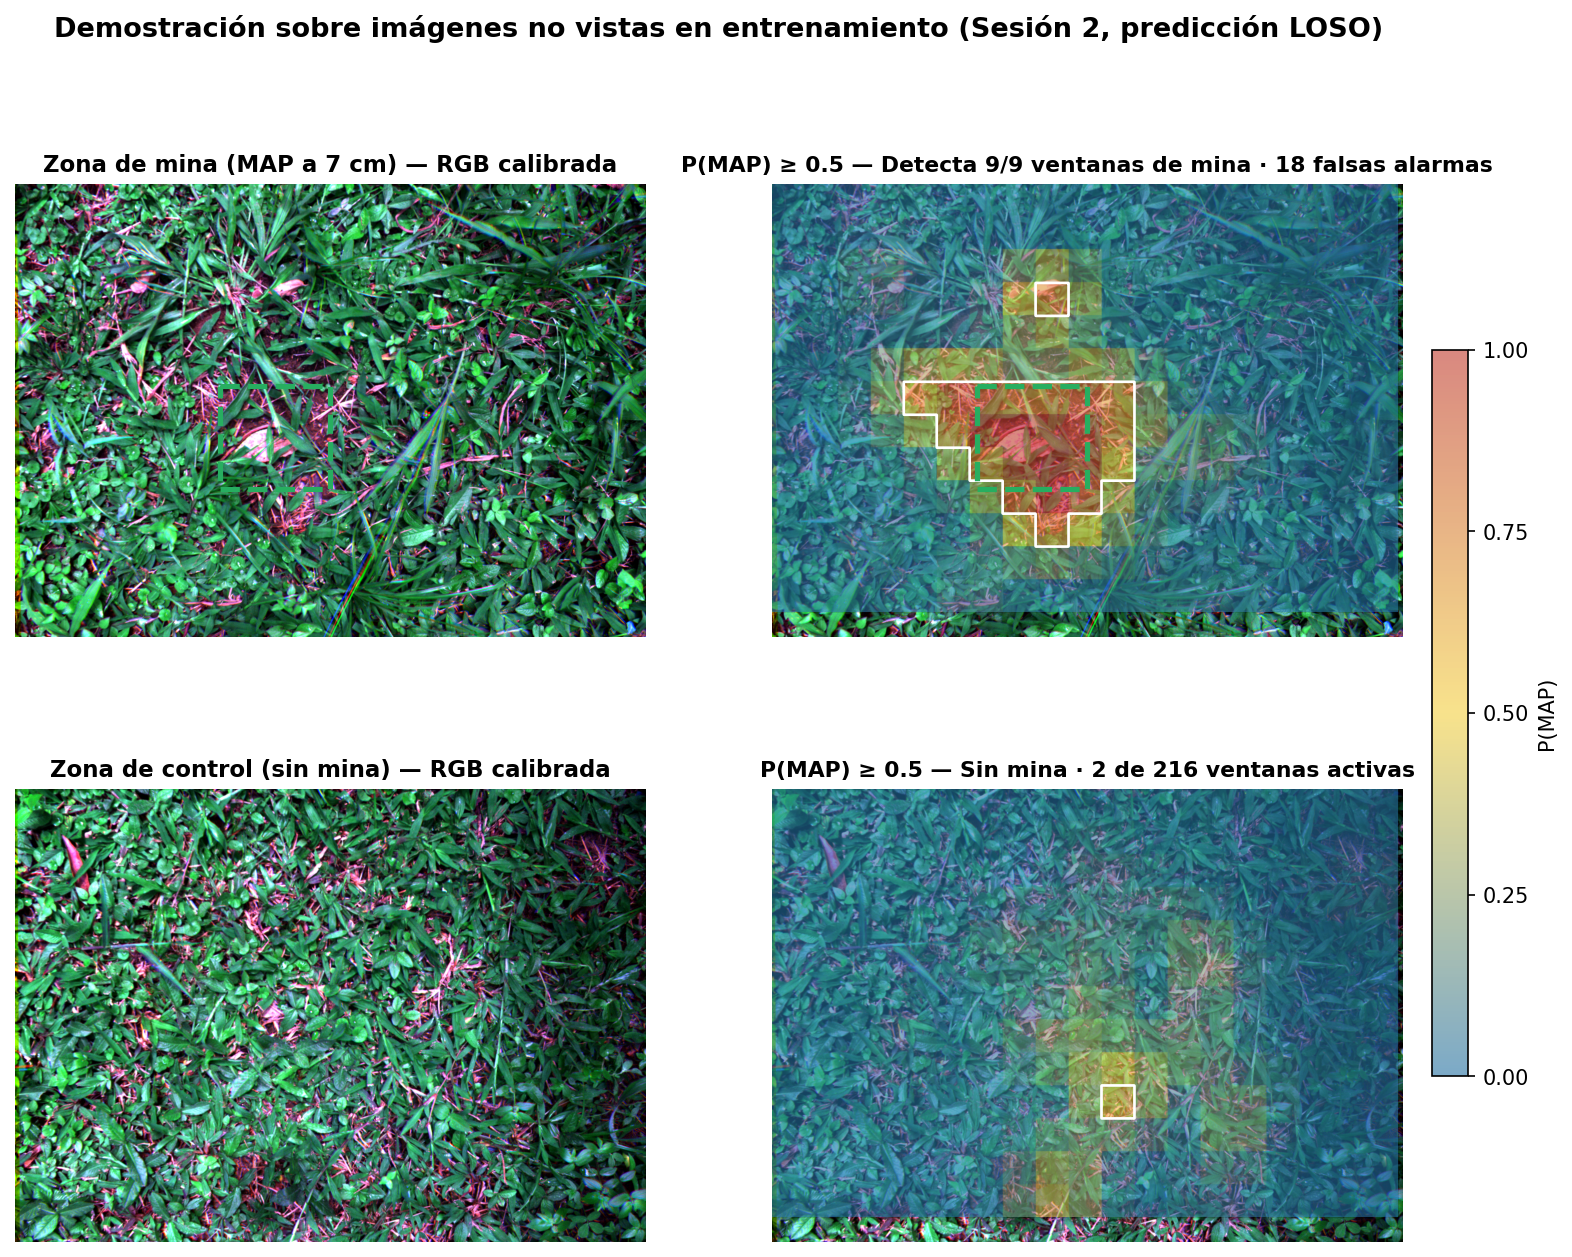
\includegraphics[width=\textwidth]{figuras/demo_no_vista.png}
  \caption{Demostración del modelo final sobre dos imágenes no vistas en
    entrenamiento (Sesión~2; predicción \ac{LOSO}, es decir, el modelo se entrenó
    sin la Sesión~2). \textit{Fila superior:} zona de mina (\ac{MAP} a 7~cm).
    \textit{Fila inferior:} zona de control sin mina. \textit{Izquierda:} RGB
    calibrada (bounding box de la \ac{MAP} en verde discontinuo).
    \textit{Derecha:} probabilidad de \ac{MAP} superpuesta (azul = baja, rojo =
    alta) con el contorno del umbral~0.5. La probabilidad alta se concentra sobre
    la mina y queda casi ausente en la zona de control.}
  \label{fig:mapa}

  {\footnotesize Fuente: elaboración propia.}
\end{figure}

% -------------------------------------------------------------
\section{Generalización a emplazamientos no vistos}
\label{sec:lozo}

\textbf{Objetivo.} La validación \ac{LOSO} deja fuera una sesión, pero las mismas
ocho zonas físicas de mina se fotografían en las seis sesiones. Cabe preguntarse si
el modelo aprende la \emph{firma de la mina} o memoriza esos ocho emplazamientos.
Para distinguirlo se evalúa una validación \emph{leave-one-zone-out} (LOZO): se deja
fuera del entrenamiento una zona de mina completa (sus seis sesiones) y se prueba
sobre ella, de modo que el modelo nunca vio ese emplazamiento.

\textbf{Metodología.} Mismo modelo final que en la
Sección~\ref{sec:modelo_final} (EasyEnsemble~x10 con las top-70 características
seleccionadas por ganancia de XGBoost dentro de cada pliegue, submuestreo 1:1); solo
cambia el agrupamiento del pliegue ---por emplazamiento físico en lugar de por
sesión--- para una comparación controlada.

\begin{table}[H]
\centering
\caption{Comparación de esquemas de validación (modelo final: EasyEnsemble~x10, top-70 características).}
\label{tab:lozo}
\small
\begin{tabular}{lc}
\toprule
\textbf{Esquema de validación} & \textbf{AUC} \\
\midrule
\ac{LOSO} (deja una sesión fuera) & $0.947 \pm 0.007$ \\
LOZO (deja un emplazamiento fuera) & $0.933 \pm 0.021$ \\
\bottomrule
\end{tabular}

  {\footnotesize Fuente: elaboración propia.}
\end{table}

\textbf{Resultados.} Al dejar fuera un emplazamiento completo, el \ac{AUC} apenas
desciende ($0.947 \to 0.933$, $-0.014$), dentro de la variabilidad entre pliegues,
y se mantiene entre 0.899 y 0.961 en las ocho zonas. La caída es marginal: si el
modelo memorizara los ocho sitios, su rendimiento sobre un emplazamiento no visto se
desplomaría, lo que no ocurre. Esto indica que el modelo aprende la firma espectral
del fenómeno ---perturbación del suelo y estrés vegetal--- y \textbf{generaliza a emplazamientos no vistos} bajo las condiciones ya
observadas, de forma complementaria a la robustez ante nuevas condiciones de
captura que evalúa la validación \ac{LOSO}. La comparación se centra en el \ac{AUC} por ser independiente tanto del umbral como de la composición del conjunto de prueba.

% -------------------------------------------------------------
\section{Rendimiento por sesión y condiciones de captura}
\label{sec:condiciones}

\textbf{Objetivo.} Evaluar si la hora, la humedad o la radiación solar afectan el
\ac{AUC}.

\textbf{Metodología.} Se relaciona el \ac{AUC} por sesión del modelo final con las
condiciones de captura registradas. Con solo seis sesiones se hace una inspección
cualitativa, sin coeficiente de correlación (que carecería de potencia estadística).

\begin{table}[H]
\centering
\caption{\ac{AUC} por sesión vs.\ condiciones de captura (ordenado por hora).}
\label{tab:condiciones}
\small
\begin{tabular}{ccccc}
\toprule
\textbf{Sesión} & \textbf{Hora} & \textbf{HR (\%)} &
\textbf{Rad. (W/m\textsuperscript{2})} & \textbf{AUC} \\
\midrule
S6 & 07:30 & 84.5 & 161.5 & 0.958 \\
S3 & 12:34 & 60.7 & 346.7 & 0.946 \\
S2 & 13:10 & 72.8 & 778.7 & 0.936 \\
S7 & 16:40 & 65.5 & 143.9 & 0.948 \\
S5 & 17:17 & 63.6 & 73.3  & 0.950 \\
S4 & 17:21 & 61.8 & 64.5  & 0.942 \\
\bottomrule
\end{tabular}

  {\footnotesize Fuente: elaboración propia.}
\end{table}

\textbf{Análisis.} Según la Tabla~\ref{tab:condiciones}, el \ac{AUC} varía poco (0.936--0.958) y \emph{no} sigue un
patrón con la hora ni la radiación: S6 a las 07:30 (sol rasante) obtiene el
\ac{AUC} más alto, comparable al de mediodía. La inspección cualitativa indica
que la firma multiespectral es \emph{estable} dentro del rango
horario del protocolo, a diferencia de la señal térmica que requiere ventanas
temporales específicas.

% -------------------------------------------------------------
\section{Rendimiento por profundidad de enterramiento}
\label{sec:profundidad}

\textbf{Objetivo.} Analizar el desempeño según la profundidad (1, 3, 5, 7~cm).

\textbf{Metodología.} Las ventanas de prueba del modelo final se reagrupan por la
profundidad de su zona y se recalculan las métricas en cada subgrupo; es el mismo
modelo, sin reentrenar.

\begin{table}[H]
\centering
\caption{Métricas \ac{LOSO} por profundidad (modelo final).}
\label{tab:profundidad}
\small
\begin{tabular}{cccc}
\toprule
\textbf{Profundidad} & \textbf{AUC} & \textbf{Sens} & \textbf{Spec} \\
\midrule
\SI{1}{cm} & 0.942 & 0.875 & 0.858 \\
\SI{3}{cm} & 0.914 & 0.880 & 0.813 \\
\SI{5}{cm} & 0.928 & 0.835 & 0.855 \\
\SI{7}{cm} & 0.915 & 0.707 & 0.923 \\
\bottomrule
\end{tabular}

  {\footnotesize Fuente: elaboración propia.}
\end{table}

\textbf{Análisis.} La \textbf{sensibilidad cae con la profundidad} (Tabla~\ref{tab:profundidad})
($0.875$ a \SI{1}{cm} $\to$ $0.707$ a \SI{7}{cm}), coherente con la física: a
menor profundidad, mayor perturbación del suelo y del estrés vegetal, señales más
detectables. En la Figura~\ref{fig:profundidad}, la línea negra es el promedio
\ac{LOSO} del \ac{AUC} y las de colores cada sesión: el \ac{AUC} se mantiene estable
(entre 0.91 y 0.94), pues la pérdida de rendimiento con la profundidad se manifiesta
en la sensibilidad (Tabla~\ref{tab:profundidad}), no en el \ac{AUC}. A \SI{7}{cm} la detección es la más
difícil, aunque el \ac{AUC} permanece muy por encima del azar. Esto refuerza que
la señal proviene de la perturbación superficial del enterramiento.

\begin{figure}[H]
  \centering
  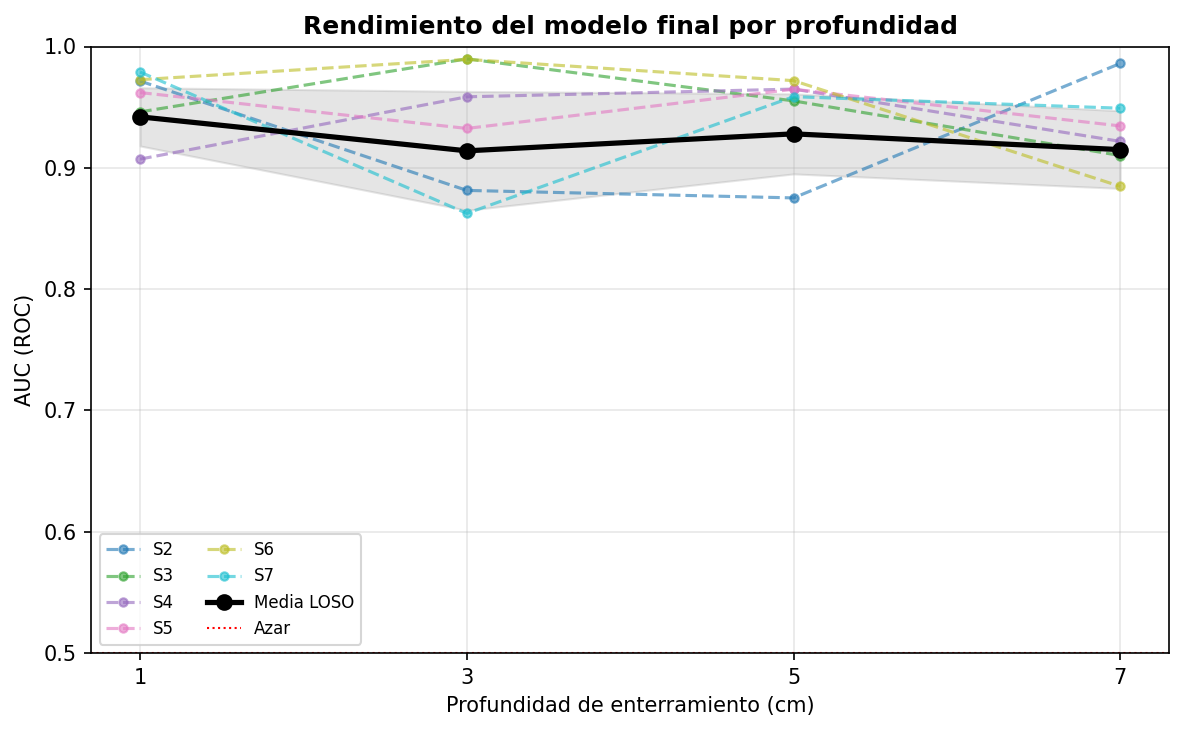
\includegraphics[width=0.85\textwidth]{figuras/p7_profundidad.png}
  \caption{\ac{AUC} por profundidad. Línea negra: promedio \ac{LOSO};
    líneas de color: cada sesión.}
  \label{fig:profundidad}

  {\footnotesize Fuente: elaboración propia.}
\end{figure}

% -------------------------------------------------------------
\section{Falsos positivos vs objetos de interferencia}
\label{sec:fp_objetos}
\label{sec:analisis_fp}

\textbf{Objetivo.} Determinar si los objetos de interferencia (botella, lata,
piedra) son la causa de los falsos positivos.

\textbf{Metodología.} Cada falso positivo del modelo final (ventana sin mina
clasificada como mina) se etiqueta según dónde cae ---sobre un objeto de
interferencia o sobre el fondo de suelo perturbado---, y se compara contra una
variante que fuerza una cuota de objetos en el submuestreo.

\textbf{Resultados.} De los 1\,363 falsos positivos en zonas de mina, solo el
\textbf{6.8\,\% caen sobre objetos} (Botella 57, Lata 17, Piedra 19) y el
\textbf{93.2\,\% sobre el fondo} ---el suelo perturbado alrededor de la mina,
cuyo borde difuso se extiende más allá del bounding box
(Figura~\ref{fig:fp_comp}). El objeto que más confunde es la \textbf{botella}.

\begin{figure}[H]
  \centering
  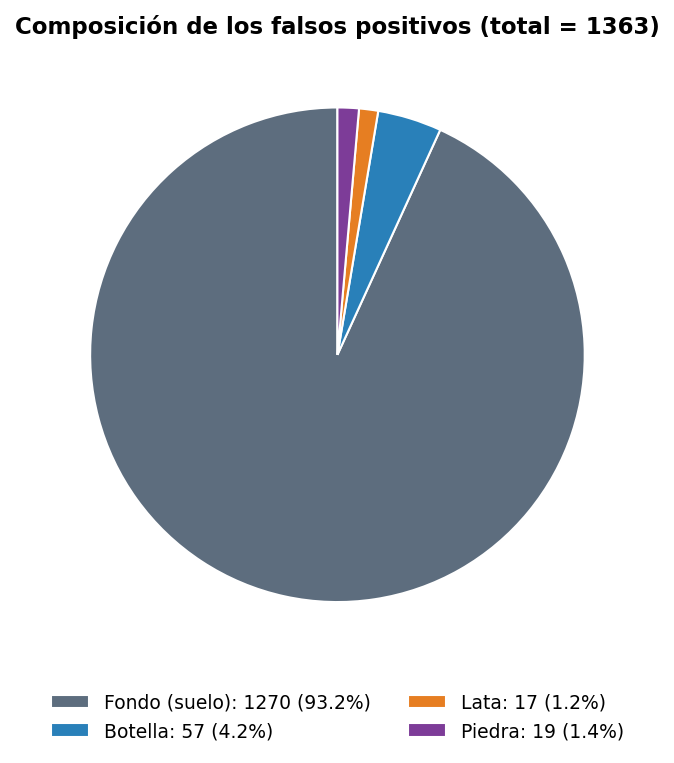
\includegraphics[width=0.62\textwidth]{figuras/p8_composicion.png}
  \caption{Composición de los falsos positivos del modelo final: el 93\,\% cae
    sobre el fondo (suelo perturbado) y solo el 6.8\,\% sobre objetos.}
  \label{fig:fp_comp}

  {\footnotesize Fuente: elaboración propia.}
\end{figure}

\textbf{Dónde falla el sistema.} Como casi todos los falsos
positivos están en suelo perturbado/desnudo y no en los objetos, el sistema
\emph{falla más en zonas de suelo removido o sin vegetación}, que se parecen a la
perturbación de una mina. En cambio, en \emph{áreas de vegetación homogénea} su
desempeño es mejor. Es una limitación honesta y a la vez una guía de uso. La
Figura~\ref{fig:fp_espacial} lo ilustra sobre una imagen: los falsos positivos se
reparten por el suelo de la zona y solo unos pocos caen cerca de los objetos.

\begin{figure}[H]
  \centering
  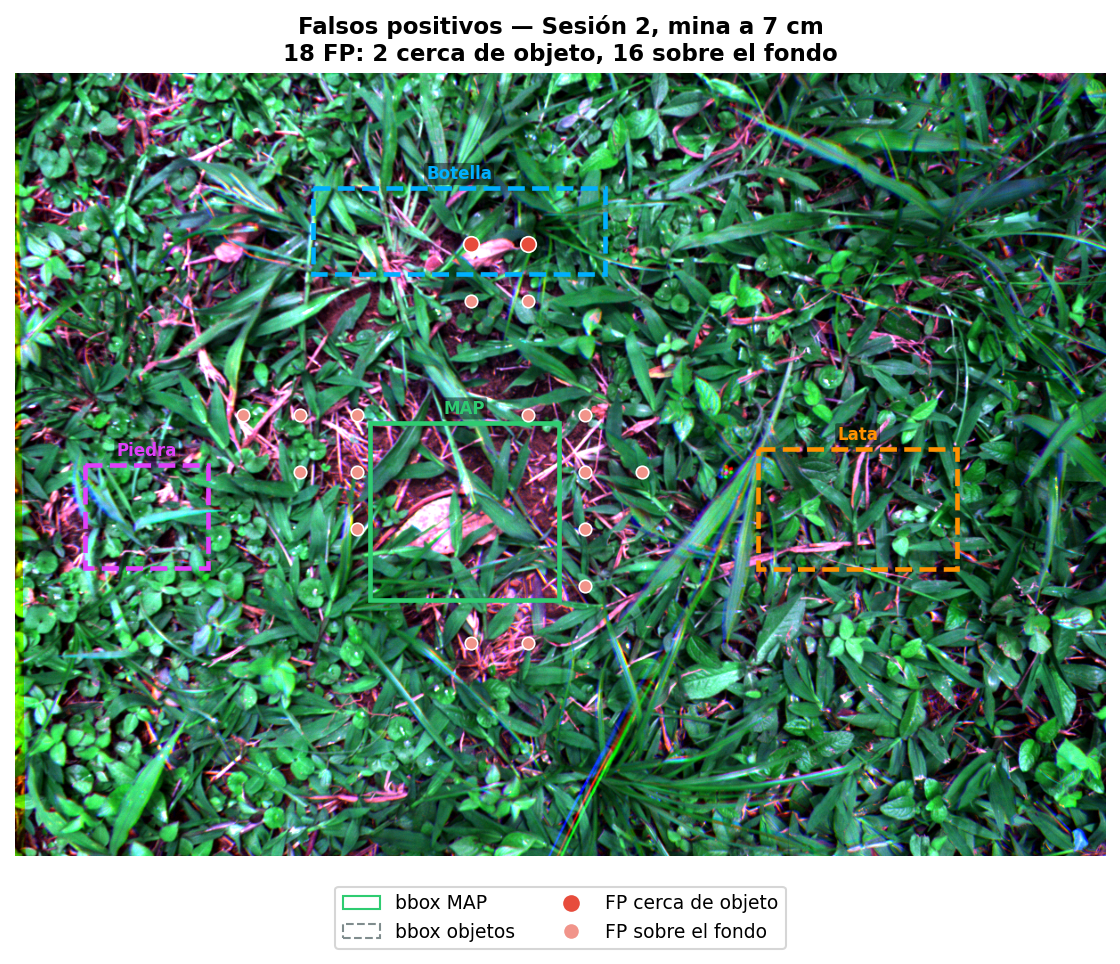
\includegraphics[width=0.78\textwidth]{figuras/fp_ejemplo.png}
  \caption{Ejemplo de falsos positivos sobre una imagen (Sesión~2, mina a 7~cm;
    predicción \ac{LOSO}, imagen no usada en el entrenamiento de ese fold). De los
    18 falsos positivos, solo 2 caen cerca de un objeto y 16 sobre el fondo,
    coherente con el conjunto.}
  \label{fig:fp_espacial}

  {\footnotesize Fuente: elaboración propia.}
\end{figure}

\textbf{Experimento: cuota de objetos.} Se evaluó forzar una cuota de objetos
(\emph{hard-negative mining}) en el submuestreo, para que el clasificador
aprendiera mejor a rechazarlos. La comparación limpia mostró que \textbf{no
ayuda} (Figura~\ref{fig:fp_cuota}): no reduce los FP sobre objetos (93 vs.\ 97)
y empeora levemente las métricas globales. La razón es coherente con lo anterior:
los objetos no son la fuente principal de falsas alarmas, así que
sobre-representarlos no ataca el problema. El modelo final usa submuestreo
aleatorio 1:1 (sin cuota). Un clasificador multiclase que distinga explícitamente
la \ac{MAP} de estos objetos queda como trabajo futuro
(Sección~\ref{sec:trabajos_futuros}).

\begin{figure}[H]
  \centering
  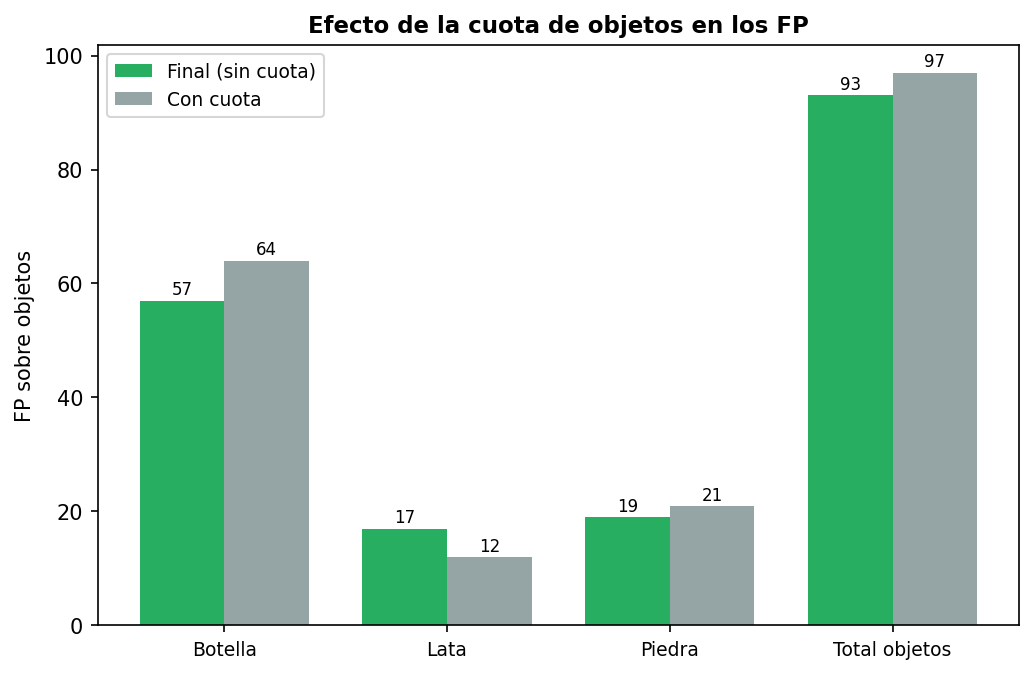
\includegraphics[width=0.75\textwidth]{figuras/p8_cuota.png}
  \caption{Efecto de la cuota de objetos: forzarla no reduce los FP sobre objetos
    (93 vs.\ 97) frente al modelo final sin cuota.}
  \label{fig:fp_cuota}

  {\footnotesize Fuente: elaboración propia.}
\end{figure}

% -------------------------------------------------------------
\section{Discusión general}
\label{sec:discusion}

La Tabla~\ref{tab:progresion} resume la progresión metodológica.

\begin{table}[H]
\centering
\caption{Progresión metodológica (S2--S7, umbral~0.5).}
\label{tab:progresion}
\small
\begin{tabular}{lccc}
\toprule
\textbf{Configuración} & \textbf{AUC} & \textbf{Sens} & \textbf{FP/mina} \\
\midrule
Random Forest, 378 características (base) & 0.915 & 0.805 & 5.29 \\
XGBoost, 378 características & 0.941 & 0.817 & 4.15 \\
EasyEnsemble, 378 características & 0.945 & 0.832 & 4.16 \\
\textbf{EasyEnsemble, top-70 (modelo final)} & \textbf{0.947} & \textbf{0.823} &
\textbf{4.16} \\
\bottomrule
\end{tabular}

  {\footnotesize Fuente: elaboración propia.}
\end{table}

El sistema final alcanza \textbf{AUC~=~0.947} con \ac{LOSO}, una ganancia de
$+0.032$ sobre la línea base (\ac{RF}, 0.915). El \emph{pipeline} completo
(calibración, alineación, extracción e inferencia) tarda entre 5 y 8~minutos por
sesión, suficiente para análisis post-captura en campo.

\textbf{Comparación con el estado del arte multiespectral.} El trabajo más
comparable es el de Silva~\etal{} \cite{silva2019}, que también detecta minas
enterradas con una cámara multiespectral y características estadísticas. Sin
embargo, sus experimentos se realizaron en \emph{cajones de arena de laboratorio}
y campo controlado, con minas enterradas pocos minutos antes de la captura
---\emph{sin señal crónica acumulada}--- y un dataset balanceado artificialmente
con partición aleatoria, alcanzando 97\,\% de exactitud. Notablemente, su sistema
\emph{no detectaba la perturbación del suelo}: justamente la señal que este
trabajo explota. En contraste, aquí se trabaja en \textbf{campo real con
vegetación en crecimiento libre ($\sim$6 meses), minas enterradas a 1--7~cm con
señal crónica, desbalance real 30:1 y validación \ac{LOSO} sin fuga de datos}.
Qiu~\etal{} \cite{qiu2023} usan una cámara multiespectral en \ac{UAV} con
\ac{NIR} y Red Edge (confirmando el valor de esas bandas), pero detectan minas en
\emph{superficie} (visibles) con una red convolucional; aquí las minas están
\emph{enterradas} (invisibles) y se detectan por su señal indirecta.

\subsection{Relación con el trabajo previo del grupo PSI}

Tenorio~\etal{} \cite{tenorio2024} es el antecedente directo dentro del grupo
\ac{PSI}: termografía infrarroja sobre \ac{UAV}, mismo terreno y tipo de mina,
con sensibilidad del 82.4\,\%. La sensibilidad obtenida aquí (82.3\,\%) es de un
nivel similar, pero \textbf{ambos trabajos no son directamente comparables}: miden
fenómenos físicos distintos ---el contraste térmico del enterramiento frente al
estrés vegetal y la anomalía del suelo---, con sensores y regímenes de validación
diferentes; además, la sensibilidad reportada corresponde en cada caso a un punto
de operación particular ---no a una medida global como el \ac{AUC}---, de modo que
dos valores cercanos no implican un rendimiento equivalente.
Los trabajos son \textbf{complementarios}: la señal térmica es aguda pero
depende de una ventana temporal estrecha (hora del día, condiciones de captura),
mientras que la señal multiespectral es más estable en el tiempo por basarse en un
efecto crónico. Una diferencia experimental clave es
que en este trabajo los \textbf{objetos de interferencia se incluyeron a
propósito} (botella, lata y piedra enterradas a la misma profundidad que la mina)
como variable controlada para medir la confusión, mientras que el estudio térmico
solo contaba con los objetos naturalmente presentes en la zona (principalmente
piedras). Por eso, fusionar ambas modalidades ---señal térmica aguda y señal
multiespectral crónica--- es una línea de trabajo natural para el grupo.

% ============================================================
%  CAPÍTULO 5 — CONCLUSIONES
% ============================================================
\chapter{Conclusiones}
\label{cap:conclusiones}

En este capítulo se presentan las conclusiones del trabajo, organizadas
por objetivo específico, seguidas de los alcances y limitaciones del sistema,
los productos de la investigación y las líneas de trabajo futuro.

% -------------------------------------------------------------
\section{Conclusiones por objetivo}

\textbf{Objetivo 1: Construcción de la base de datos.}
Se construyó una base de datos de imágenes multiespectrales de \ac{MAP}
emuladas enterradas en suelo arenoso con vegetación limitada a \SI{1}{m}
de altura, siguiendo un protocolo reproducible de captura estacionaria mediante
una estructura de soporte de \ac{PVC} diseñada para este fin. La base de datos oficial
comprende seis sesiones de campo (S2--S7) con ocho zonas de mina por sesión
(profundidades de 1, 3, 5 y 7~cm, con dos réplicas por profundidad) y entre
una y cuatro zonas de control (una en S2, cuatro en S3--S7), totalizando
14\,901 ventanas. Las condiciones de iluminación resultaron ser el factor más determinante
para la consistencia de las firmas espectrales entre sesiones: la hora de
captura, la uniformidad de la luz y la humedad del suelo explican en gran
medida las diferencias entre S1 y las sesiones posteriores. Esta observación
motivó el ajuste del protocolo a partir de S2 y la exclusión de la Sesión~1
de la base de datos oficial.

\textbf{Objetivo 2: Procesamiento de imágenes multiespectrales.}
Se implementó un \textit{pipeline} automatizado de calibración radiométrica
mediante \ac{CRP}, alineación de bandas por \ac{SIFT}+RANSAC y extracción de
378 características estadísticas sobre ventanas de $128\times128$ píxeles. Durante la implementación se encontró una limitación no documentada
de la MicaSense RedEdge-MX: la umbralización de Otsu falla en la banda
Red Edge porque la vegetación y el panel de calibración tienen reflectancias
similares a \SI{717}{nm}. Detectar la máscara en la banda Roja y aplicarla
a las cinco bandas resolvió el problema y mejoró la consistencia de la
calibración radiométrica.

\textbf{Objetivo 3: Reconocimiento de patrones.}
El etiquetado preciso del groundtruth ---una ventana es positiva solo si su centro
cae dentro del bounding box de la \ac{MAP}--- produjo 487 ventanas positivas frente
a 14\,414 negativas (desbalance 30:1). El análisis de importancia mostró que las
bandas \ac{NIR} y Red Edge contribuyen de forma clara a la discriminación: de las
70 características del modelo final, 36 (la mitad) involucran \ac{NIR} o Red Edge. Tras comparar \ac{RF},
\ac{SVM}, XGBoost y EasyEnsemble, se eligió \textbf{EasyEnsemble~x10 XGBoost}
(submuestreo 1:1 para corregir el desbalance 30:1) con las \textbf{top-70
características} de mayor ganancia de XGBoost, alcanzando
\textbf{AUC~=~0.947~$\pm$~0.007} y sensibilidad del 82.3\,\% a umbral~0.5. Frente a
la línea base (\ac{RF}, 378 características, AUC~=~0.915), la ganancia total es de
$+$0.032 AUC.

\textbf{Objetivo 4: Evaluación del sistema.}
El modelo detectó minas en las cuatro profundidades evaluadas. La sensibilidad
disminuye con la profundidad ---del 87.5\,\% a \SI{1}{cm} al 70.7\,\% a
\SI{7}{cm}---, coherente con que la señal proviene de la perturbación superficial
del suelo y del estrés vegetal: a mayor profundidad, menor alteración detectable.
Aun así, el \ac{AUC} se mantiene alto en todas las profundidades (0.91--0.94), muy
por encima del azar. Respecto a los falsos positivos, el \textbf{93\,\%} no se
asocia a los objetos de interferencia (botella, lata, piedra), sino al borde
difuso del suelo perturbado alrededor de la mina; el clasificador no confunde
sistemáticamente esos objetos con la \ac{MAP}.

% -------------------------------------------------------------
\section{Alcances y limitaciones}

\subsection{Alcances}

\begin{itemize}
  \item El sistema alcanzó AUC~=~0.947 con Sens(0.5)~=~82.3\,\% (umbral 0.5)
    sobre \ac{MAP} emuladas en suelo arenoso con vegetación hasta \SI{1}{m},
    usando EasyEnsemble~x10 XGBoost con las top-70 características seleccionadas
    por ganancia de XGBoost bajo validación LOSO.
  \item El \textit{pipeline} cubre todo el proceso sin intervención manual,
    desde la captura hasta el mapa de probabilidades. Esto lo hace
    directamente aplicable en futuras campañas de campo.
  \item Las 378 características pueden reducirse a las top-70 sin pérdida de
    rendimiento (incluso ligeramente superior a usar las 378). El vector de
    entrada se reduce a menos de una quinta parte.
  \item El análisis de importancia mostró que las bandas Red Edge y \ac{NIR}
    contribuyen a la detección: 36 de las 70 características del modelo final las
    involucran.
  \item La validación \ac{LOSO} evita que ventanas de la misma sesión aparezcan en
    entrenamiento y prueba al mismo tiempo, lo que haría los resultados
    irrealmente optimistas. Además, una validación que deja fuera cada
    emplazamiento físico (\textit{leave-one-zone-out}, AUC~=~0.933 frente a 0.947)
    indica que el modelo generaliza a sitios no vistos bajo condiciones ya
    observadas.
\end{itemize}

\subsection{Limitaciones}

\begin{itemize}
  \item La base de datos usa minas emuladas en suelo arenoso bajo condiciones
    controladas. No se ha probado el sistema con minas reales ni en terrenos
    con mayor heterogeneidad de suelo o vegetación.
  \item El sistema solo distingue entre mina y no-mina. Aunque el análisis
    de FP incluyó objetos de interferencia (botella, lata, piedra),
    clasificarlos por separado no fue parte del trabajo.
  \item El modelo responde a la firma espectral de estrés vegetal y
    perturbación del suelo asociadas a la mina. Zonas con vegetación
    naturalmente deteriorada o suelo removido por causas ajenas pueden
    presentar firmas similares, contribuyendo a las falsas alarmas.
  \item Las condiciones extremas de iluminación pueden afectar las firmas
    espectrales, como evidenció la Sesión~1 (HR~=~90.5\,\%, ángulo solar
    rasante). Dentro del rango del protocolo (S2--S7), el análisis por
    sesión no mostró una correlación fuerte entre la hora de captura y el
    AUC, aunque el sistema requiere un protocolo de captura estricto para
    evitar condiciones atípicas.
  \item El paralaje entre los cinco lentes de la MicaSense a \SI{1}{m}
    genera un desalineamiento residual que la homografía global no puede
    corregir completamente sobre vegetación tridimensional.
  \item El ratio positivos:negativos de 1:30 limita la cantidad de ventanas de
    mina disponibles; más sesiones o más minas por sesión mejorarían la robustez
    del modelo.
\end{itemize}

% -------------------------------------------------------------
\section{Productos del trabajo de investigación}

A partir del desarrollo de este trabajo de grado se obtuvieron los
siguientes productos:

\begin{itemize}
  \item \textbf{Documento de trabajo de grado.} El presente documento,
    que constituye la memoria técnica completa del sistema desarrollado.

  \item \textbf{Base de datos de imágenes multiespectrales.} Base de datos de
    imágenes de \ac{MAP} emuladas enterradas en suelo arenoso con vegetación
    limitada, adquiridas con la cámara MicaSense RedEdge-MX
    a \SI{1}{m} de altura en el campus de la Universidad del Valle.
    La base de datos incluye ocho zonas de mina por sesión (profundidades de
    1, 3, 5 y 7~cm) y cuatro zonas de control, con seis sesiones de
    campo bajo distintas condiciones ambientales.

  \item \textbf{Código fuente del \textit{pipeline} de procesamiento.}
    Implementación completa en Python del sistema de preprocesamiento
    radiométrico y geométrico, extracción de características espectrales
    y clasificación con validación \ac{LOSO}. 
\end{itemize}

% -------------------------------------------------------------
\section{Trabajos futuros}
\label{sec:trabajos_futuros}

Con base en los resultados y limitaciones identificadas, se proponen las
siguientes líneas de trabajo futuro:

\begin{enumerate}
  \item \textbf{Clasificación multiclase y reducción de falsos positivos.}
    Aprovechar las anotaciones de cuatro clases (MAP, Botella, Lata, Piedra)
    ya disponibles en la base de datos para desarrollar un clasificador capaz de
    distinguir entre \ac{MAP}, objetos inofensivos y suelo limpio, reduciendo
    así la tasa de falsos positivos del sistema actual. El análisis espectral
    por clase (Figura~\ref{fig:firmas_espectrales}) muestra que las cuatro
    clases presentan patrones parcialmente diferenciables, particularmente en
    las bandas NIR y Red Edge, lo que respalda la factibilidad de este enfoque.

  \item \textbf{Montaje en UAV.} Escalar el sistema a un \ac{UAV} para
    validar la operación en condiciones de vuelo real, considerando el
    movimiento de la plataforma y su efecto sobre la alineación de bandas.
    Los resultados del trabajo previo del grupo \ac{PSI} \cite{tenorio2024}
    en la misma plataforma constituyen una referencia directa para este paso.

  \item \textbf{Fusión de sensores.} Integrar la información multiespectral
    con datos termográficos del enfoque previo del grupo \ac{PSI}
    \cite{tenorio2024} para explorar si la fusión de ambas modalidades
    ---señal crónica multiespectral y señal aguda térmica--- mejora la
    tasa de detección y reduce los falsos positivos.

  \item \textbf{Análisis de estabilidad espectral temporal.} Estudiar cómo
    evolucionan las firmas espectrales sobre las \ac{MAP} a lo largo de
    semanas y meses, para identificar la ventana temporal óptima de detección
    basada en estrés vegetal crónico y determinar si el efecto aumenta,
    se estabiliza o decrece con el tiempo.

  \item \textbf{Generalización a terrenos heterogéneos.} Validar el sistema
    en terrenos con mayor densidad vegetal, vegetación más alta, o suelos
    con diferente textura y composición, para establecer los límites
    operativos del enfoque multiespectral.

  \item \textbf{Incertidumbre del sensor y sesgo del NDRE.} Incorporar la
    incertidumbre de la calibración radiométrica en el análisis de resultados,
    en particular el sesgo residual del \ac{NDRE} documentado en este trabajo,
    para cuantificar su efecto sobre las características más discriminativas.
\end{enumerate}


% -- REFERENCIAS ----------------------------------------------
\cleardoublepage
\phantomsection
\addcontentsline{toc}{chapter}{Referencias}
\bibliography{referencias}

% -- ANEXOS ---------------------------------------------------
\appendix
% ============================================================
%  ANEXOS
% ============================================================

\chapter{Especificaciones técnicas de la cámara MicaSense RedEdge-MX}
\label{anx:camara}

La Tabla~\ref{tab:specs_camara} resume las especificaciones técnicas
principales de la cámara MicaSense RedEdge-MX empleada en este trabajo.

\begin{table}[H]
\centering
\caption{Especificaciones técnicas de la cámara MicaSense RedEdge-MX}
\label{tab:specs_camara}
\begin{tabular}{ll}
\toprule
\textbf{Parámetro}              & \textbf{Valor} \\
\midrule
Número de bandas                & 5 \\
Resolución por banda            & 1280 $\times$ 960 px (1.2 Mpx) \\
Tamaño del sensor               & 4.8 mm $\times$ 3.6 mm \\
Tamaño de píxel                 & 3.75 \si{\micro m} \\
Distancia focal                 & 5.5 mm \\
Campo de visión horizontal      & 47.2° \\
Campo de visión vertical        & 35.4° \\
Lentes                          & 5 objetivos físicamente separados \\
Interfaz de captura             & API HTTP REST (\texttt{192.168.10.254}) \\
Formato de salida               & TIFF sin comprimir (16 bits) \\
Sensor de irradiancia           & DLS 2 (Downwelling Light Sensor) \\
Alimentación                    & 4.2--15.8 V, consumo típico 4 W \\
Masa                            & 232 g \\
\midrule
\multicolumn{2}{c}{\textit{Bandas espectrales}} \\
\midrule
Banda 1 — Azul (Blue)           & Centro: 475 nm, FWHM: 32 nm \\
Banda 2 — Verde (Green)         & Centro: 560 nm, FWHM: 27 nm \\
Banda 3 — Rojo (Red)            & Centro: 668 nm, FWHM: 16 nm \\
Banda 4 — Red Edge              & Centro: 717 nm, FWHM: 12 nm \\
Banda 5 — NIR                   & Centro: 842 nm, FWHM: 57 nm \\
\bottomrule
\end{tabular}

  {\footnotesize Fuente: elaboración propia.}
\end{table}

% ============================================================

\chapter{Código fuente del \textit{pipeline} de procesamiento}
\label{anx:codigo}

La Tabla~\ref{tab:scripts} describe los scripts principales del
\textit{pipeline} de preprocesamiento, extracción de características y
clasificación que conforman el sistema implementado.

\begin{table}[H]
\centering
\caption{Scripts principales del \textit{pipeline} de procesamiento}
\label{tab:scripts}
\small
\begin{tabular}{p{6.0cm}p{6.5cm}}
\toprule
\textbf{Script} & \textbf{Descripción} \\
\midrule
\texttt{pipeline\_completo.py}
  & Orquestador principal. Ejecuta las tres etapas secuencialmente para una sesión de campo. \\[4pt]
\texttt{preprocesamiento.py}
  & Calibración radiométrica mediante \ac{CRP}, alineación de bandas por \ac{SIFT}+RANSAC y recorte de bordes. \\[4pt]
\texttt{extraccion\_features.py}
  & Extracción de ventanas ($128\times128$~px, 50\,\% solapamiento), cálculo de 40+ índices espectrales y 9 estadísticas por índice. \\[4pt]
\texttt{clasificador\_rf.py}
  & Entrenamiento del \ac{RF} con validación cruzada estratificada. \\[4pt]
\texttt{evaluar\_loso.py}
  & Validación \ac{LOSO} con $N$ sesiones. Genera métricas por pliegue y promedio. \\[4pt]
\texttt{extraccion\_segmentada.py}
  & Re-etiquetado de ventanas por bounding box usando anotaciones Roboflow. \\[4pt]
\texttt{metricas\_modelo\_final.py}
  & Entrenamiento y evaluación del modelo final: EasyEnsemble x10 XGBoost,
    top-70 características seleccionadas por XGBoost, validación \ac{LOSO}. \\[4pt]
\texttt{micasense\_preview\_capture.py}
  & Captura de imágenes mediante la API HTTP de la cámara MicaSense. \\
\bottomrule
\end{tabular}

  {\footnotesize Fuente: elaboración propia.}
\end{table}

% ============================================================

\chapter{Base de datos de imágenes multiespectrales}
\label{anx:dataset}

La Tabla~\ref{tab:estructura_dataset} resume la estructura del dataset
al cierre del período experimental.

\begin{table}[H]
\centering
\caption{Estructura del dataset de imágenes multiespectrales}
\label{tab:estructura_dataset}
\begin{tabular}{lc}
\toprule
\textbf{Parámetro}                      & \textbf{Valor} \\
\midrule
Sesiones oficiales (S2--S7)    & 6 \\
Zonas de mina por sesión                & 8 (2 réplicas $\times$ 4 profundidades) \\
Profundidades evaluadas                 & 1, 3, 5 y 7 cm \\
Zonas de control por sesión (S3+)       & 4 \\
Bandas espectrales por captura          & 5 (TIF, 16 bits por banda) \\
Objetos de interferencia por zona       & 3 (roca, botella de vidrio, lata) \\
Formato del dataset procesado           & CSV (una ventana por fila, 378 columnas) \\
Tamaño de ventana                       & 128 $\times$ 128 px \\
Solapamiento entre ventanas             & 50\,\% \\
\bottomrule
\end{tabular}

  {\footnotesize Fuente: elaboración propia.}
\end{table}


\end{document}
